\documentclass[a4paper]{article}

\usepackage{hyperref}
\usepackage{graphicx}
\usepackage{caption}
\usepackage{subcaption}
\usepackage{kpfonts}
\graphicspath{ {img/} }

\usepackage{amsmath}
\usepackage{bbm}
\usepackage{dsfont}
\usepackage{amsfonts}
\usepackage{amsthm}
\usepackage{mathtools}
\usepackage{gensymb}
\usepackage[margin=1in]{geometry}
\usepackage{tabto}
\usepackage{xcolor}

\geometry{rmargin=1.5in}

\makeatletter
% \renewcommand\section{\@startsection{section}{1}{\z@}%
%                                   {-3.5ex \@plus -1ex \@minus -.2ex}%
%                                   {2.3ex \@plus.2ex}%
%                                   {\normalfont\normalsize\bfseries}}
\makeatletter


\title{\Large Estimation of Laplace Series Coefficients via 2-D Numerical Quadrature}
\author{Evan Voyles}
\date{}

\newtheorem{theorem}{Th\'eor\`eme}
\newtheorem*{theorem*}{Th\'eor\`eme}
\newtheorem{exercice}{Exercice}
\newtheorem*{exercice*}{Exercice bonus}
\theoremstyle{definition}
\newtheorem{definition}{D\'efinition}
\newtheorem*{definition*}{D\'efinition}
\newtheorem{lemme}{Lemme}
\newtheorem{proposition}{Proposition}
\newtheorem*{proposition*}{Proposition}

\begin{document}

\makeatletter
\maketitle
\begin{center}
    \vspace{-.2in}
    \today
\end{center}
\makeatother

\newenvironment{norm}{
    \normalfont
}


\section{Abstract}

This paper provides an alternative approach to the computation
of Laplace Series coefficients $C_l^m$ and $S_l^m$ with algorithmic complexity $O(Nl^2)$ in time and $O(Nl^2)$ in space. We 
make use of the fact that the spherical harmonics form a complete and orthogonal set to directly
compute $C_l^m$ as a 2-dimensional integral. We estimate this integral using numerical quadrature techniques
and the resulting model is blazing fast compared to a least squares model running in $O(Nl^4$). Harnessing the structure of the 
data sets, we perform many optimization to reduce the amount of data needed to be stored in memory and save time by precomputing values of the 
associated Legendre polynomials. We explore the scalability of this algorithm when implemented in parallel and we present a high-degree model of the
ultra data set.



\section{Preliminaries}

Any sufficiently regular function defined on a sphere can be written
\begin{equation} \label{eq:f_iso}
    f(\theta, \phi) = \sum_{l = 0}^{+\infty}\sum_{m = 0}^l \bar P_l^m(\cos\theta)[C_l^m\cos m\phi + S_l^m \sin m \phi].
\end{equation}

Where $C_l^m, S_l^m$ are \textit{spherical harmonic} coefficients (also referred to as Laplace series coefficients) of 
degree \textit{l} and order \textit{m}; $\bar P_l^m$ are the fully normalized Associated Legendre Functions of degree $l$ and order $m$;
$\theta$ is the polar angle and $\phi$ is the azimuthal angle, as per ISO convention\footnote{We have chosen the ISO standard coordinate system to 
ensure the integrity of future computations. For a discussion on transforming the $(\phi, \lambda)$ coordinates provided by NASA, see Appendix A}.

The project proposal suggests computing the coefficients $C_l^m, S_l^m$ by setting up an overdetermined linear system of equations and finding the least squares
solution. Unfortunately, this problem runs in $O(Nl_{max}^4)$ time and requires about $8N(l_{max} + 1)^2$ bytes of memory. That is absurdly prohibitive. Furthermore, there 
are no \textit{self-evident} parallelization techniques to speed up computation time. In this report we propose an alternative approach to computing the Laplace series coefficients
$C_l^m$ and $S_l^m$ that runs in \textbf{$O(Nl^2)$} time complexity with trivial parallelization models.

\subsection{Laplace Series Coefficients}

The coefficients $C_l^m$ and $S_l^m$ are defined as the orthogonal projection of $f(\theta, \phi)$ onto the basis functions $Y_l^m$, 
the spherical harmonics of degree $l$ and order $m$. This definition is perfectly analagous to the fourier coefficients for $2\pi$ 
periodic functions. Written in terms of the normalized legendre polynomials, these projections are defined as:

\begin{align*}
    \label{eq:coeff}
    C_l^m &= \int_0^{2\pi}\int_0^\pi f(\theta, \phi) \bar P_l^m (\cos \theta)\cos (m \phi) \sin \theta d\theta d\phi\\
    S_l^m &= \int_0^{2\pi}\int_0^\pi f(\theta, \phi) \bar P_l^m (\cos \theta)\sin (m \phi) \sin \theta d\theta d\phi 
\end{align*}

We propose a solution to directly compute an approximation of the $C_l^m$ and $S_l^m$ using numerical integration.

\newpage

\section{Data Sets}

NASA data sets contain the altitude information for a spherical coordinate pair. The spherical coordinates can
be represented as the discretization of a 2-d rectangle with width $2\pi$ and height $\pi$. NASA's data sets contain observations
over a discretization of $[-\frac{\pi}{2}, \frac{\pi}{2}] \times [-\pi, \pi]$, represented as a $n_\theta \times n_\phi$ grid with equidistant points.

\begin{figure}[h!]
    \centering
    \begin{minipage}{.5\textwidth}
      \centering
      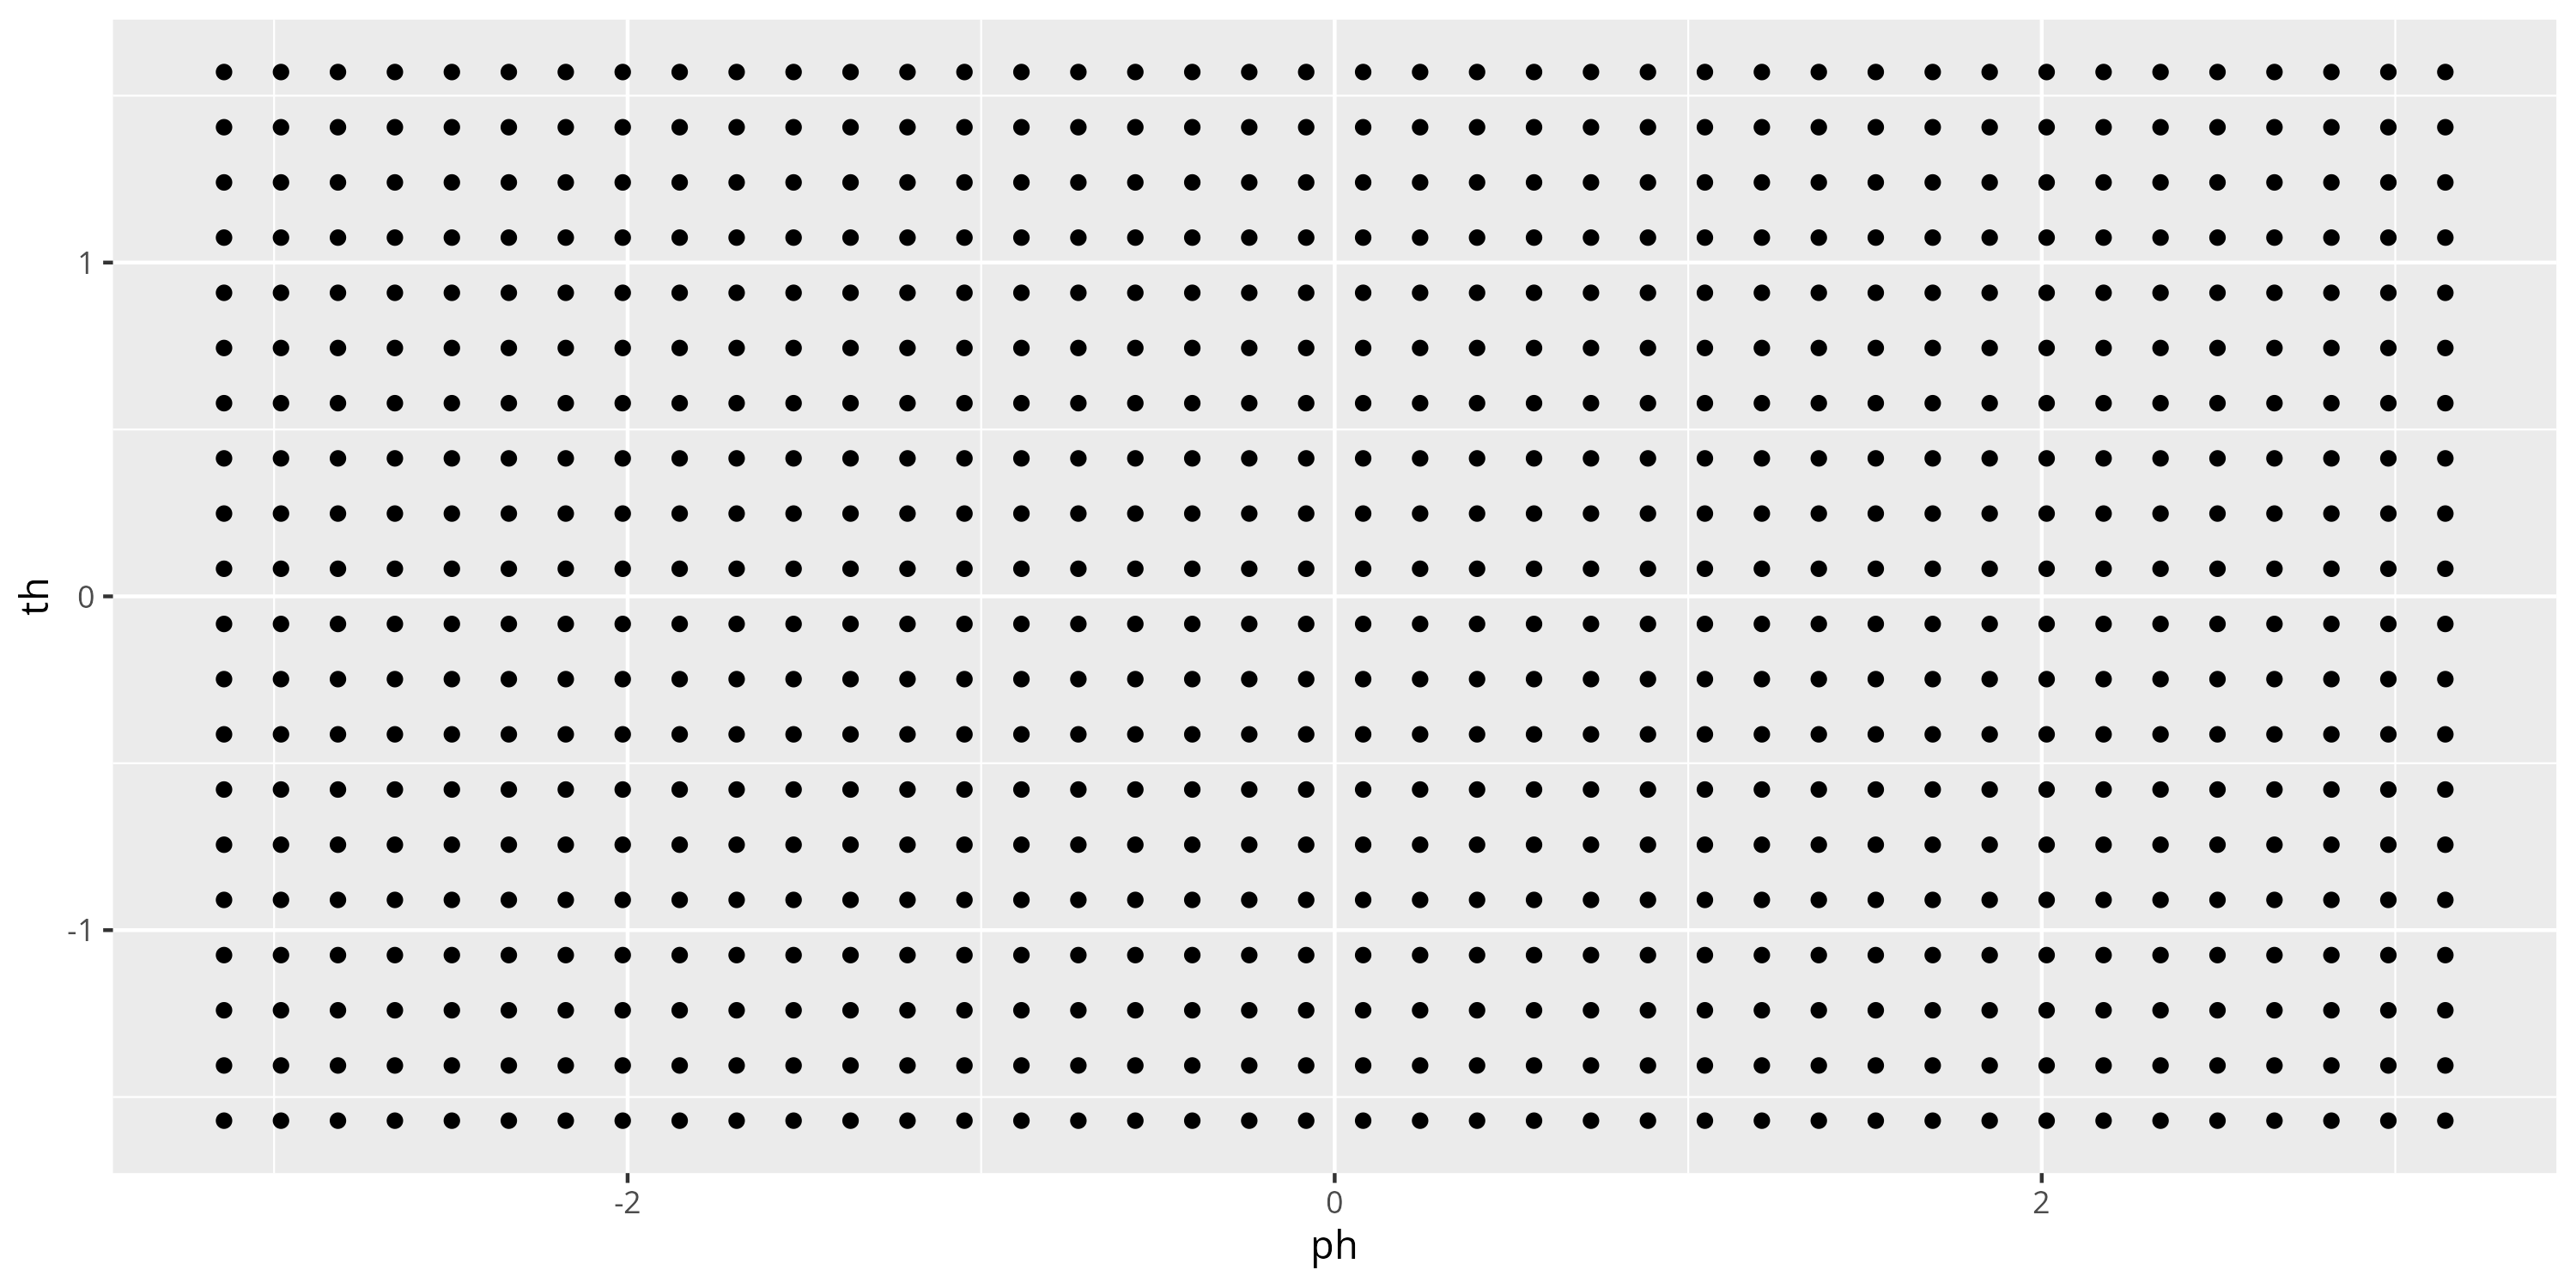
\includegraphics[width=.95\textwidth]{media/discretized_grid.png}
    %   \captionof{figure}{A figure}
      \label{fig:test1}
    \end{minipage}%
    \begin{minipage}{.5\textwidth}
      \centering
      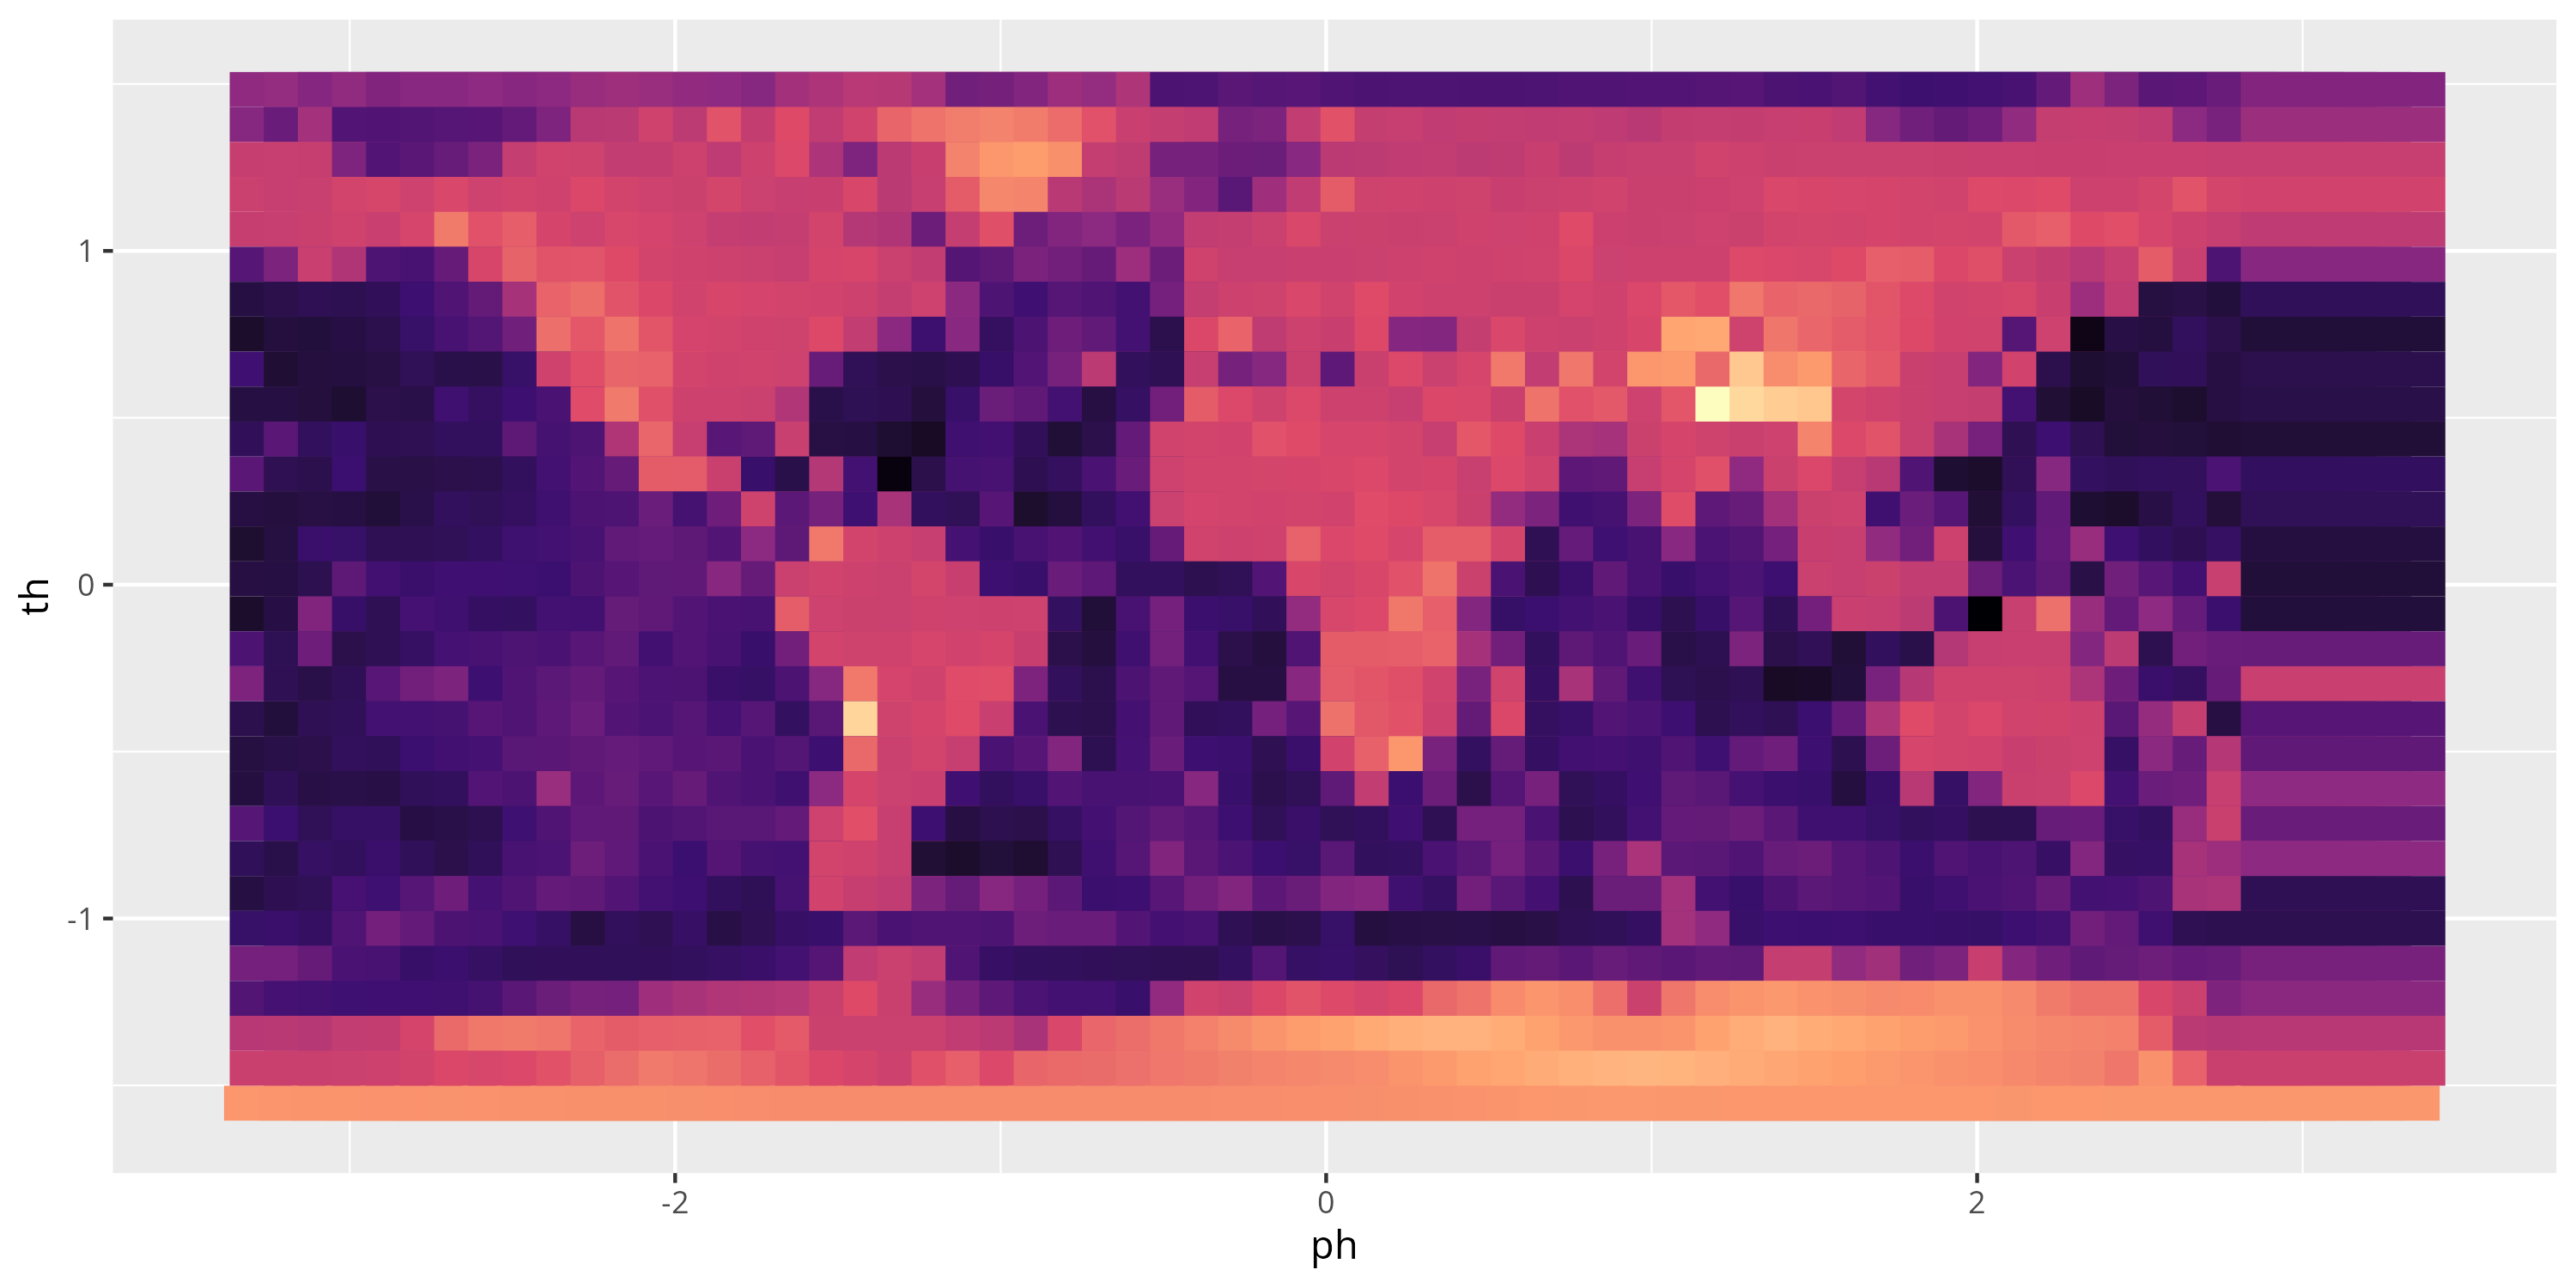
\includegraphics[width=.95\textwidth]{media/discretized_reduced.png}
    %   \captionof{figure}{Another figure}
      \label{fig:test2}
    \end{minipage}
    \caption{Discretization points (left) of a reduced data set with $n_\theta = 20$, $n_\phi = 40$. On the vertical axis we have $\theta \in [-\pi/2, \pi/2]$, or the latitude; On 
    the horizontal axis we have $\phi \in [-\pi, \pi]$, the longitude.}
\end{figure}

Due to the linear spacing, we only need to know the number of points $n_\theta$ and $n_\phi$ to recreate the spherical coordinate pairs provided 
by the data sets, allowing us to decrease the running memory footprint of our program. In order study informative analytics about our model, we first enumerate
the characteristics of each data set.

% \begin{figure}[h!]
    % \centering a
    \begin{center}
    \begin{tabular}{ c |  c  c  c }
        & $n_\theta$ & $n_\phi$ & $N$ \\ 
    \hline
    small & 180 & 360 & 64800\\
    med & 540 & 1080 & 583200\\
    hi \\
    ultra
    \end{tabular}
    \end{center}
% \end{figure}
$$\theta \in [0, \pi],\ \ \phi \in [0, \pi2]$$

We'll use these values later when we study the time it takes to compute our model.

\subsection{Visualization}

\textbf{TODO:} [ ] add 3-d maps

\section{Mathematical Model}

We define $\mathcal{M}_L$ a spherical model of degree $L$ to be the set of coefficients $$\{C_0^0, C_1^0, C_1^1, \dots, C_L^L\} \cup \{S_0^0, S_1^0, SL^L, \dots, S_L^L\}$$
 that are used in conjonction with Figure (\ref{eq:f_iso}) to provide an estimate of $f$, $\hat f$, defined as:
\begin{equation}
    \hat f(\theta, \phi; L) = \sum_{l = 0}^{L}\sum_{m = 0}^l \bar P_l^m(\cos\theta)[C_l^m\cos m\phi + S_l^m \sin m \phi].
\end{equation}

Notice that the $+\infty$ in the outer summation has been replaced with the degree of the model, $L$. We will evaluate the efficacy of the model by studying the distance between $f$ and $\hat f$
at the observations of our data set. Of notable interest will be the average absolute error (AAE) and the mean squared error (MSE):
\begin{equation}
    \label{eq:AAE}
    \mathrm{AAE}(l_{max}) = \frac{1}{N}\sum_{i = 1}^{N} |\hat f_i - f_i |, \quad MSE(l_{max}) = \frac{1}{N} \sum_{i = 1}^N (\hat f_i - f_i)^2
\end{equation}

where $\hat f_i$ denotes the estimated altitude evaluated at the $i$th data point and $f_i$ is the true observed altitude of the $i$th data point.


\subsection{Computation of Coefficients via Numerical Integration}


    
We approximate the Laplace Series coefficients via a 2 dimensional analogue of the rectangle rule.  
\begin{align*}
    C_l^m &\approx \sum_{i = 1}^{n_\phi}\sum_{j = 1}^{n_\theta} f(\theta_j, \phi_i) P_l^m (\cos \theta_j)\cos (m \phi_i) \sin \theta_j \Delta\theta \Delta\phi\\
          &\approx \Delta\theta \Delta\phi\sum_{i = 1}^{n_\phi}\cos (m \phi_i)\sum_{j = 1}^{n_\theta} f(\theta_j, \phi_i) P_l^m (\cos \theta_j) \sin \theta_j\\
    S_l^m &\approx \sum_{i = 1}^{n_\phi}\sum_{j = 1}^{n_\theta} f(\theta_j, \phi_i) P_l^m (\cos \theta_j)\sin (m \phi_i) \sin \theta_j \Delta\theta \Delta\phi\\
          &\approx \Delta\theta \Delta\phi\sum_{i = 1}^{n_\phi}\sin (m \phi_i)\sum_{j = 1}^{n_\theta} f(\theta_j, \phi_i) P_l^m (\cos \theta_j) \sin \theta_j
\end{align*}

This method computes \textit{individual} Laplace series coefficients in $O(N)$ time! Thus, computing the coefficients for a Discrete Laplace Series (DLS) of order $l$ runs in
$O(Nl^2)$. More interestingly, each $C_l^m$ or $S_l^m$ can be computed \textbf{independently} of any other coefficient. Whereas solving the linear least squares problem requires computing
every $C_l^m$ and $C_l^m$ up to a given $L$ in a single operation, this method allows us the ability to compute any arbitrary $C_l^m$ directly. Why do we care? If I alraedy have the first 500 $C_l^m$ coefficients computed
and stored in a text file, I can \textit{directly} compute the next p coefficients in $O(pN)$ time. This method allows us to also compute ranges of $C_l^m$ and $S_l^m$ without messing around
with bulky matrices taking up millions of bytes. As a consequence, there are simple yet powerful parallelization schemes that can be easily implemented to speed up computation and increase 
the performance of our models.

% \newpage
\subsection{Comparison with Linear Squares}

Let's start by exploring the small data set and benchmarking how long it takes to compute a model of degree $l$ for $l \in \{0, 2, 4, \dots, 20\}$ via 
a) an overdetermined system of linear equations b) numerical integration. Our aim in this section is to show that computing the coefficients via numerical integration
provides numerous benefits to the overall methodology and allows us to compute higher degree models with lower error more efficiently.

\subsubsection{Timing}


We experimentally corroborate the theoretical hypothesis that the least squares computation is of time complexity $O(Nl^4)$ for a data set of size $N$ and 
model degree $l$.

\begin{figure}[h!]
    \centering
    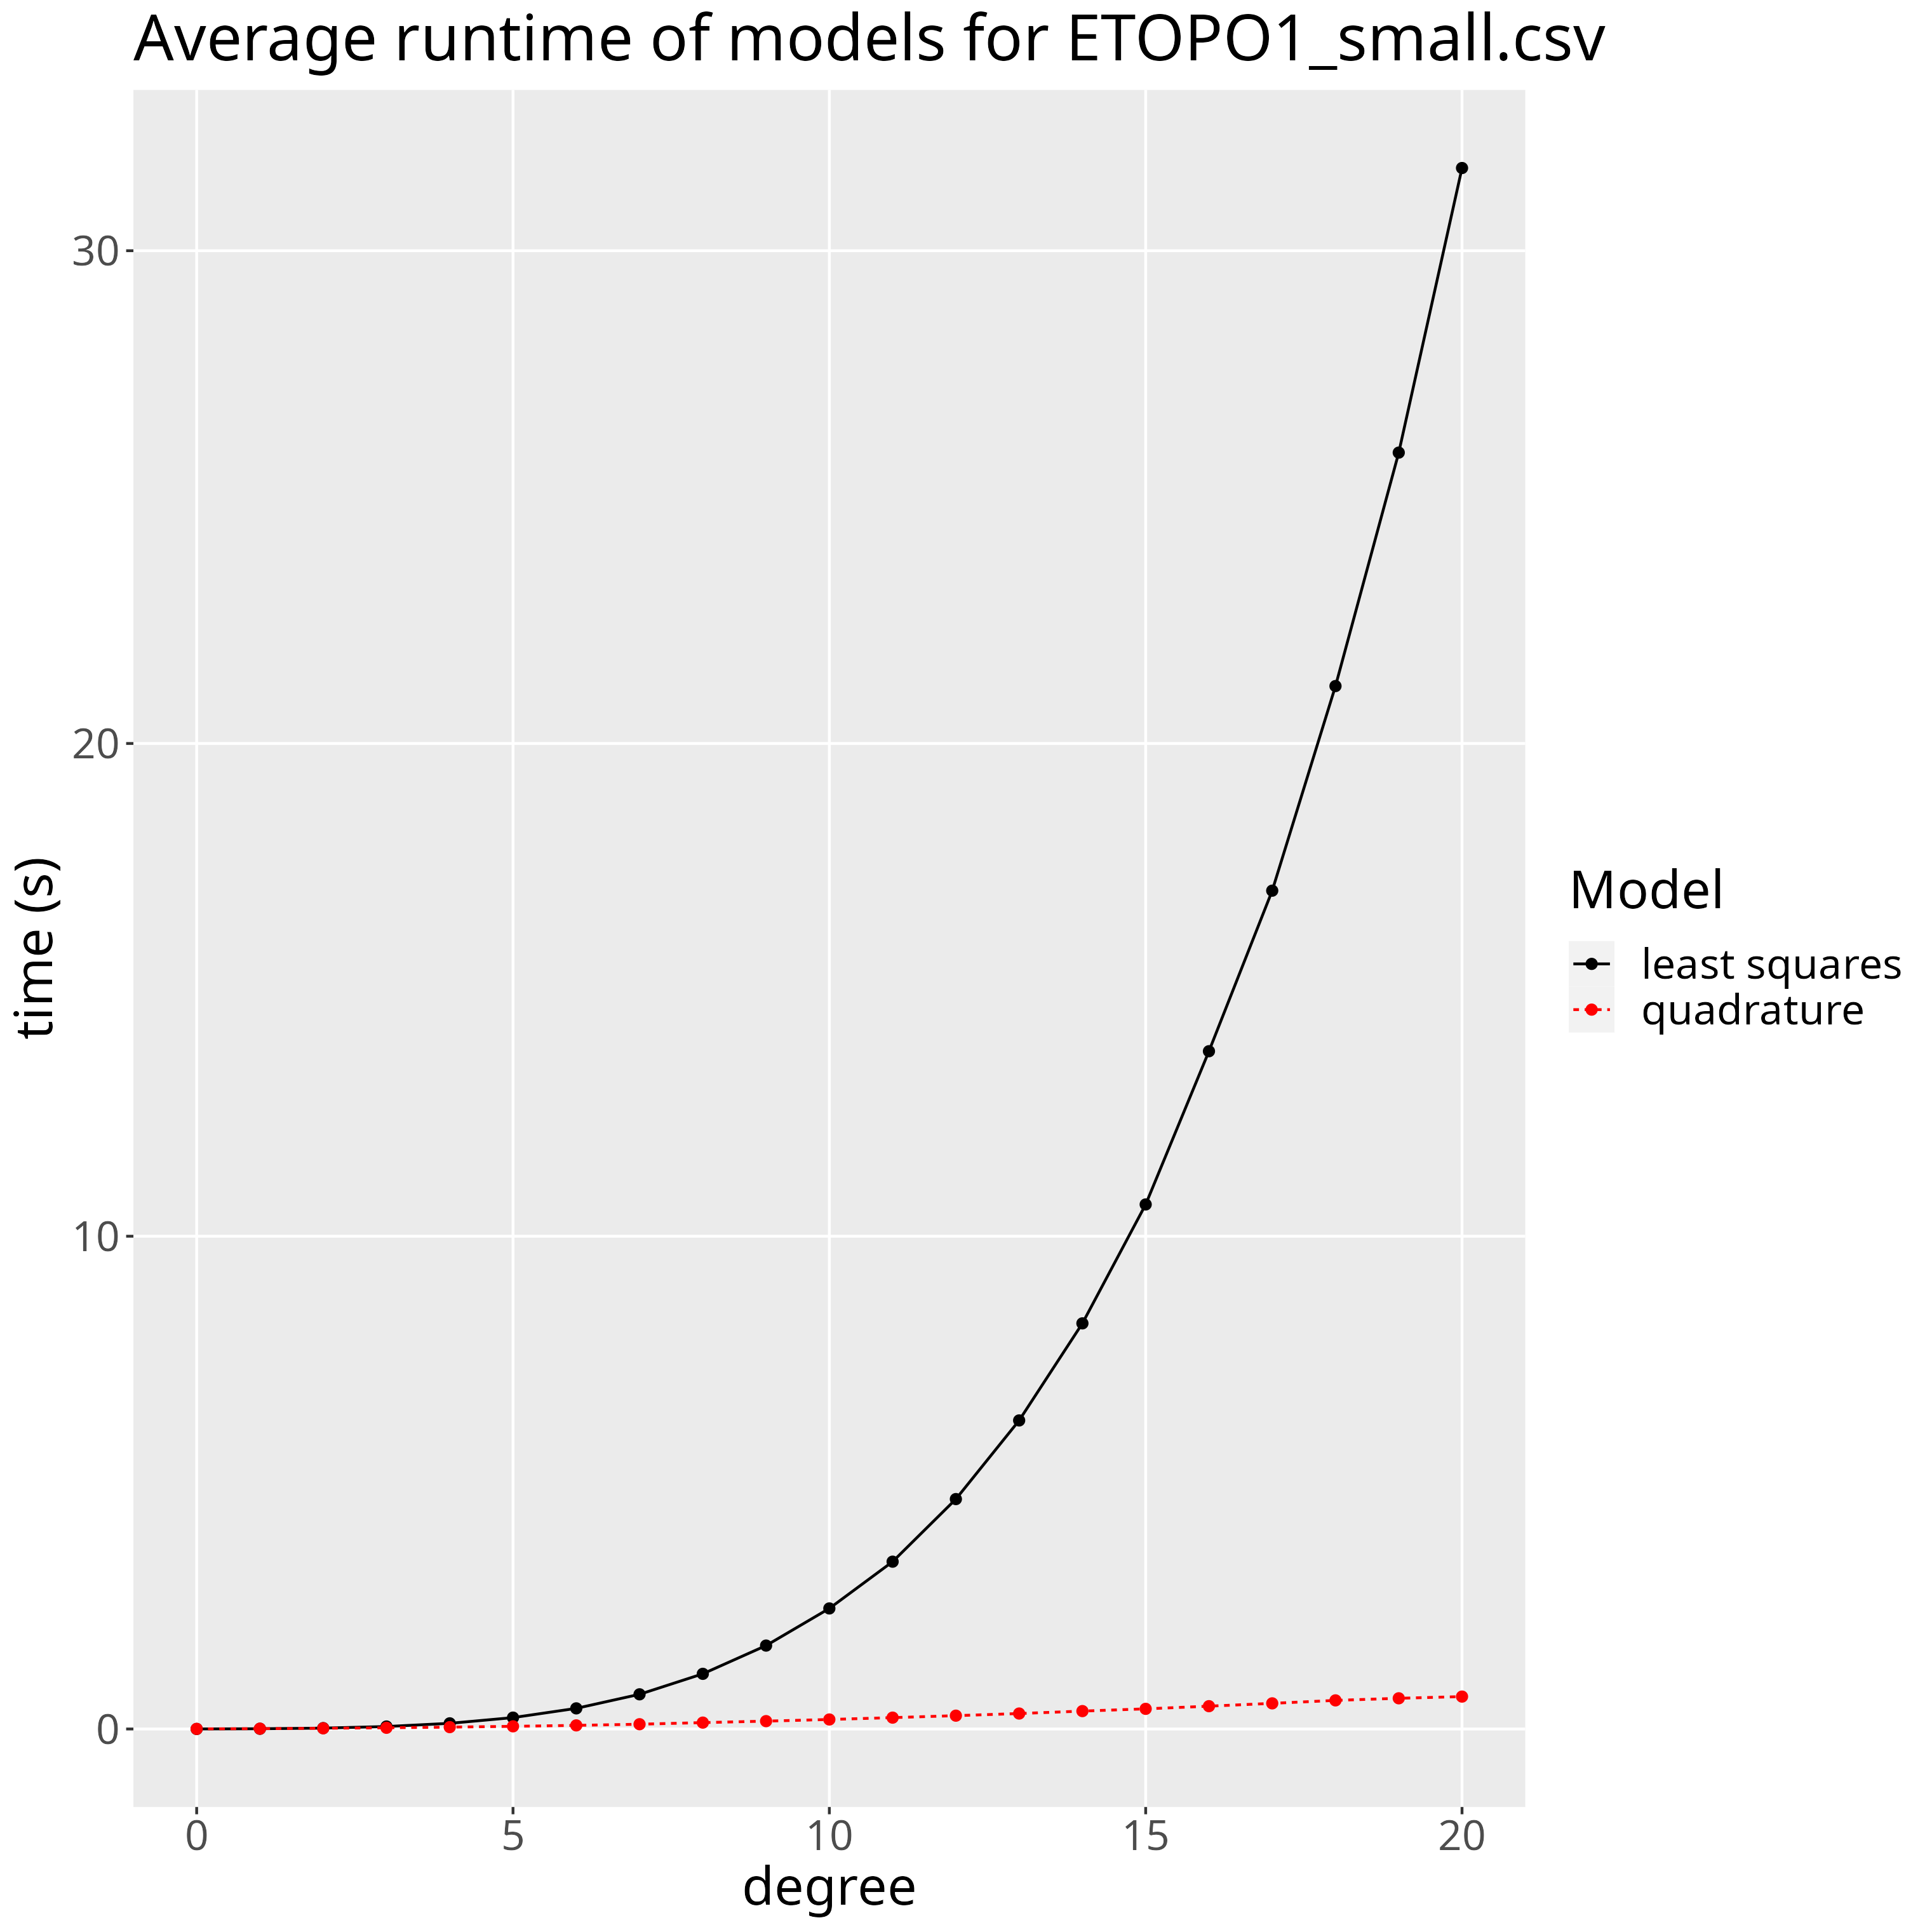
\includegraphics[width=0.5\textwidth]{media/average_runtime.png}
    \caption{A timing comparison between least squares $\in O(Nl^4)$ and numerical quadrature $\in O(Nl^2)$ to compute the coefficients $C_l^m$ and $S_l^m$ for the small ETOPO1 data set. 
    For each degree of the model Laplace coefficients were computed 5 times. Programs were run in sequential with 1 processor. TODO: Run a linear regression}
    \label{fig:runtime}
\end{figure}


When we study how long it takes to compute a model of degree 20 (Figure \ref{fig:runtime}) for the small data set we find that the least squares method takes, on average, a staggering 31.678 seconds to run. 
Coefficients computed by numerical integration, on the other hand, were generated with an average runtime of 0.656s across
5 trials. As we will see in the following analysis, a model of degree 20 is wholly incomplete to accurately represent a data set with 648000 points, and we are not 
satisfied with the runtime of the least squares method. And that's just for a small $l$. Running the algorithm in sequential for higher values of $l$ would quickly become
intractable due to its steep algorithmic complexity, especially magnified if we wanted to compute models for larger data set with millions of points (The medium data set has half a million) For a model of degree 20, numerical quadrature ran on average ~50x faster than its least squares counterpart. As the degree
of the model increases, so does the disparity between the two runtimes; at $l=20$ our algorithm runs 50 times faster but at $l = 100$ our algorithm could be running 1250 times faster.

Clearly the proposed numerical integration model is faster. But how do two models compare when it comes to average squared error? 


\newpage
\subsubsection{Model Performance}

In the least squares model, coefficients are carefully selected by minimizing the MSE of the prediction, which amounts to solving a linear system in $O(Nl^4)$ time. We are therefore,
by construction, finding optimal coefficients that should miniimze the MSE. We compare how the average abs error, the AAE, varies with
respect to the degree of the model.


\begin{figure}[h!]
    \centering
    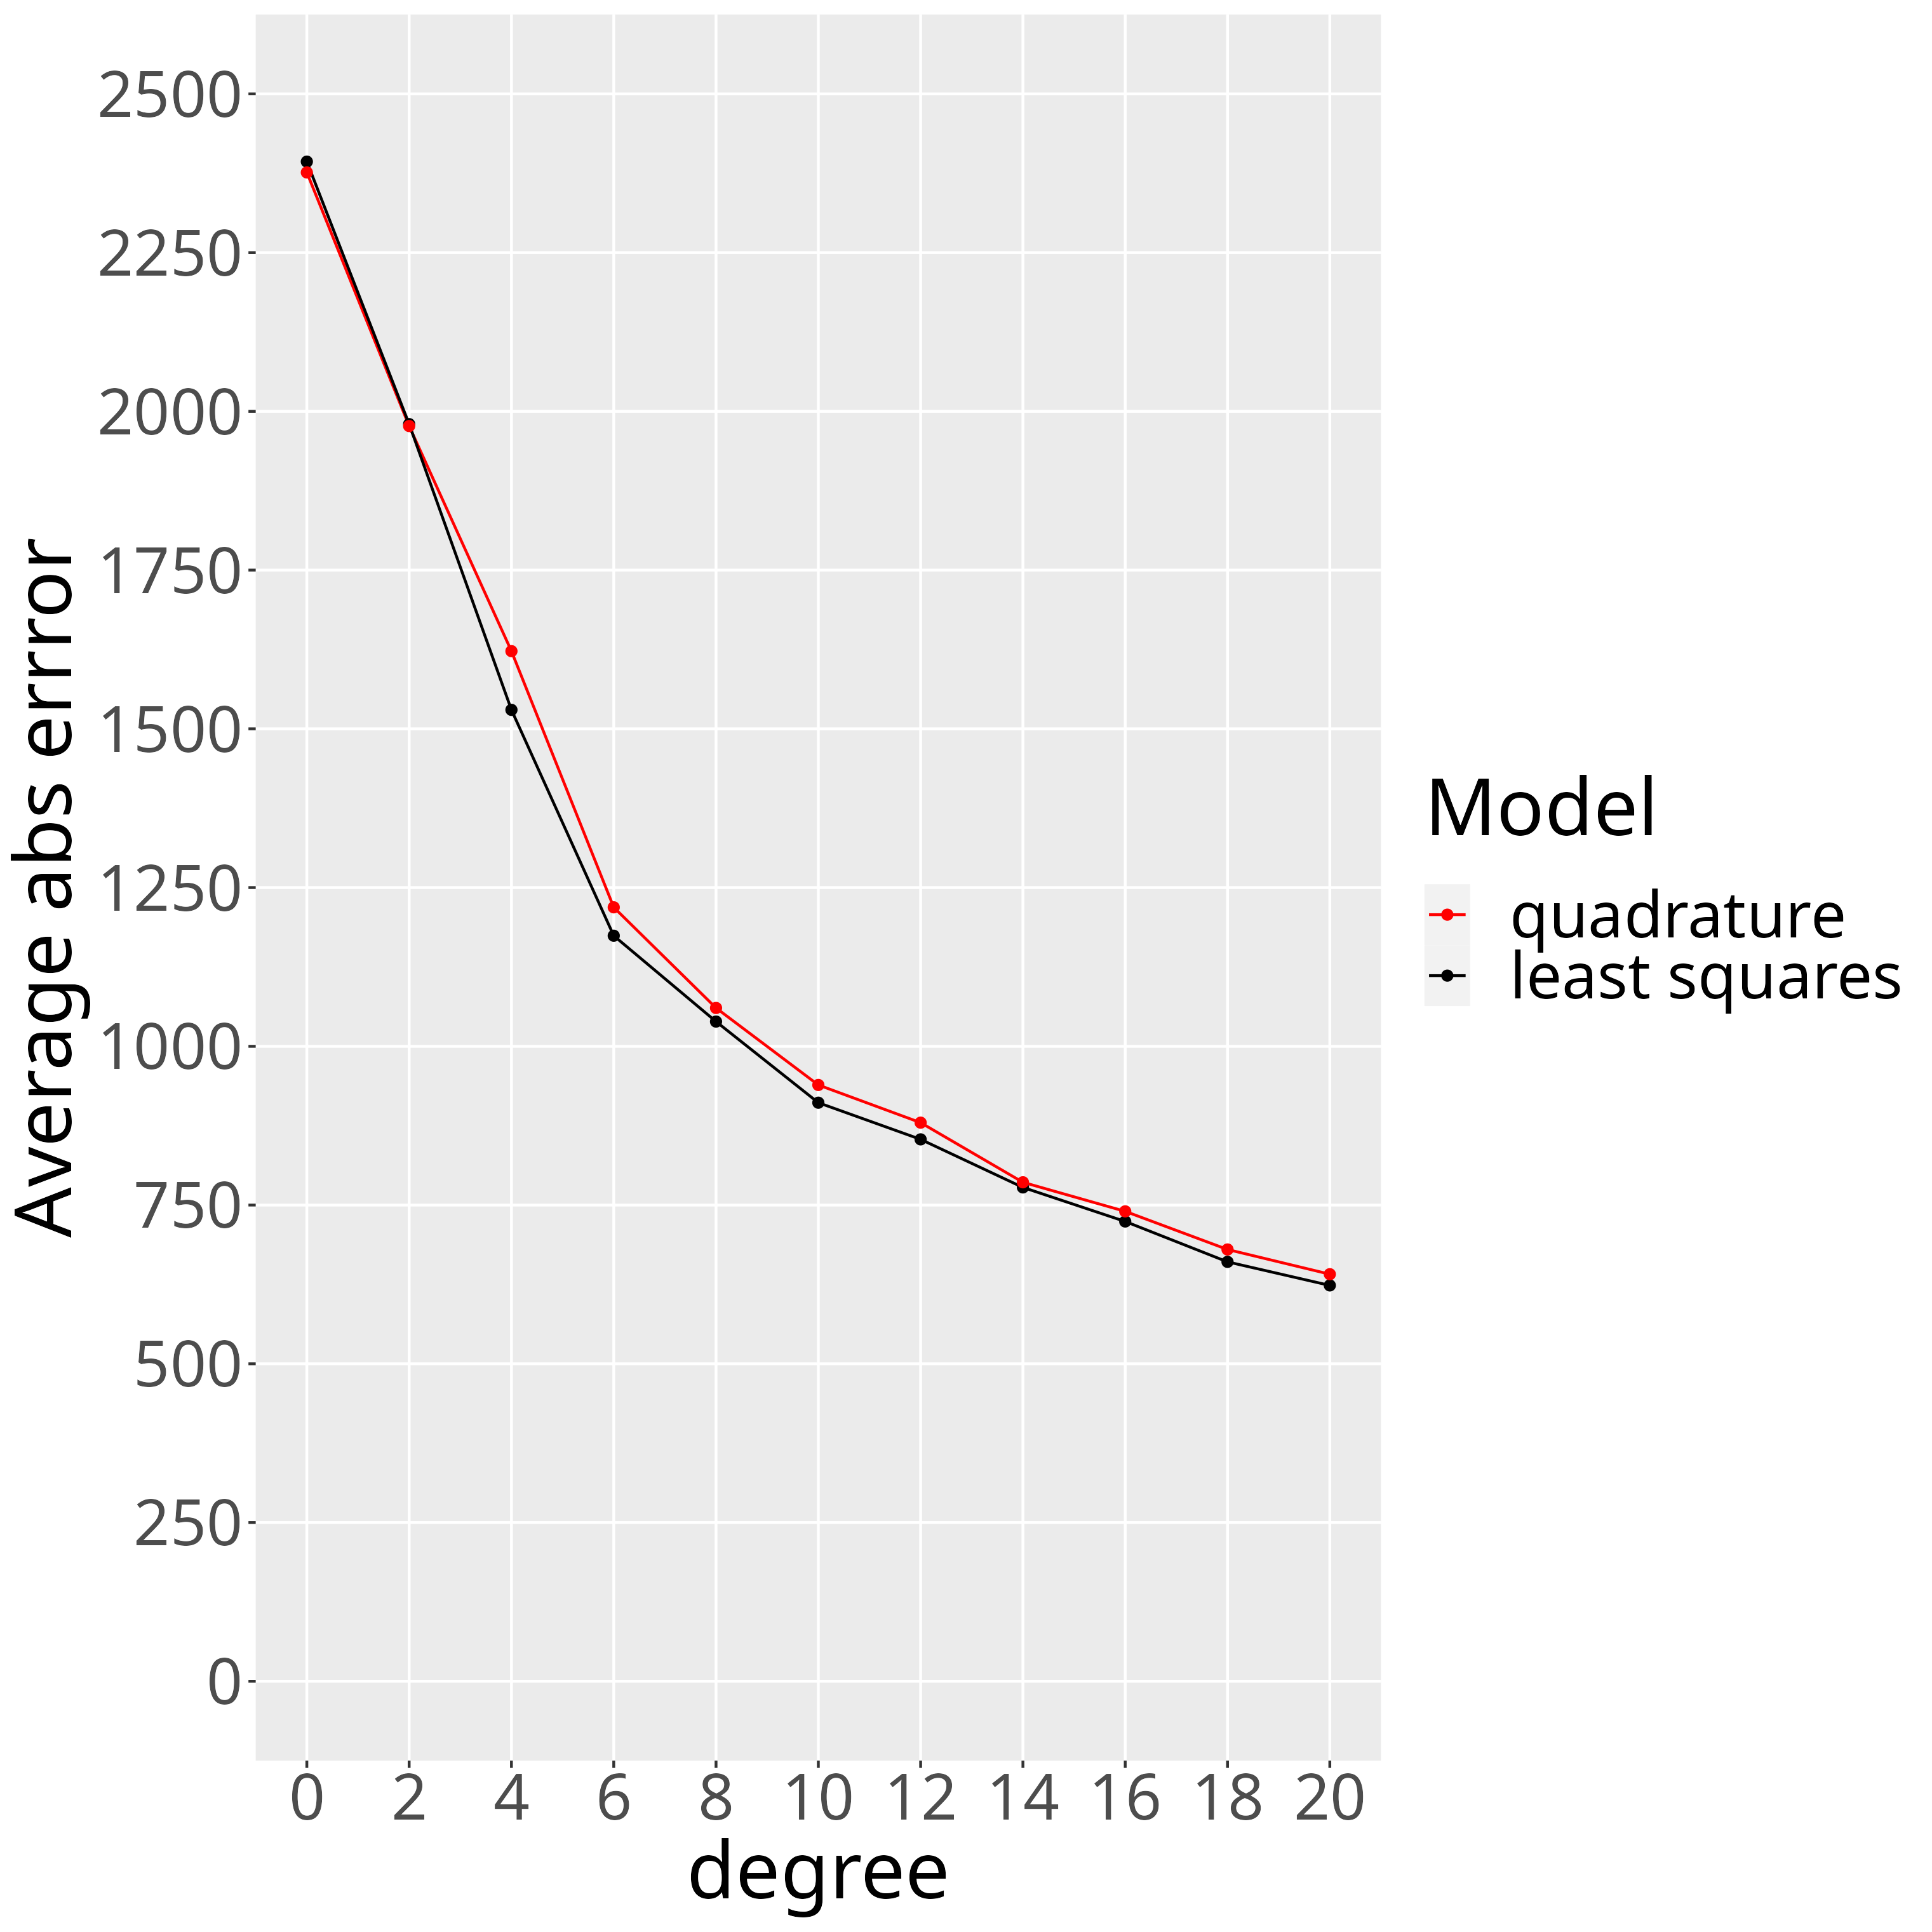
\includegraphics[width=0.6\textwidth]{media/diff_error.png}
    \caption{A Comparison between the average abs error between the least squares estimate and numerical quadrature estimate for the small ETOPO1 data set. Coefficients computed via least squares
    perform slightly better than their quadrature counter parts.}
    \label{fig:error}
\end{figure}

Perhaps surprisingly, we find that there is no significant penalty to using numerical quadrature to estimate a model's coefficients. In fact, computing the coefficients via quadrature allows us to 
create higher degree models that, running in the same time as a low-order least squares model, will have far lower average absolute error values and furthermore the distributions of the error will be
much tighter, exhibiting lower variance. In fact, as will be shown in the next section, we can run a degree 200 model using numerical integration in around 20 seconds whose average abs error
is 148.76, compared to the degree 20 model whos AAE is 641.1.

\subsubsection{Higher Degree Models}
In this section we explore the distribution of error values ($\hat f - f$) for models up to degree $l = 300$, computed for the small, medium, and high resolution data sets.

We start off by showing the evolution of the model's estimates as the degree $l$ increases

\begin{figure}[h!]
    \begin{minipage}{.245\textwidth}
        \centering
        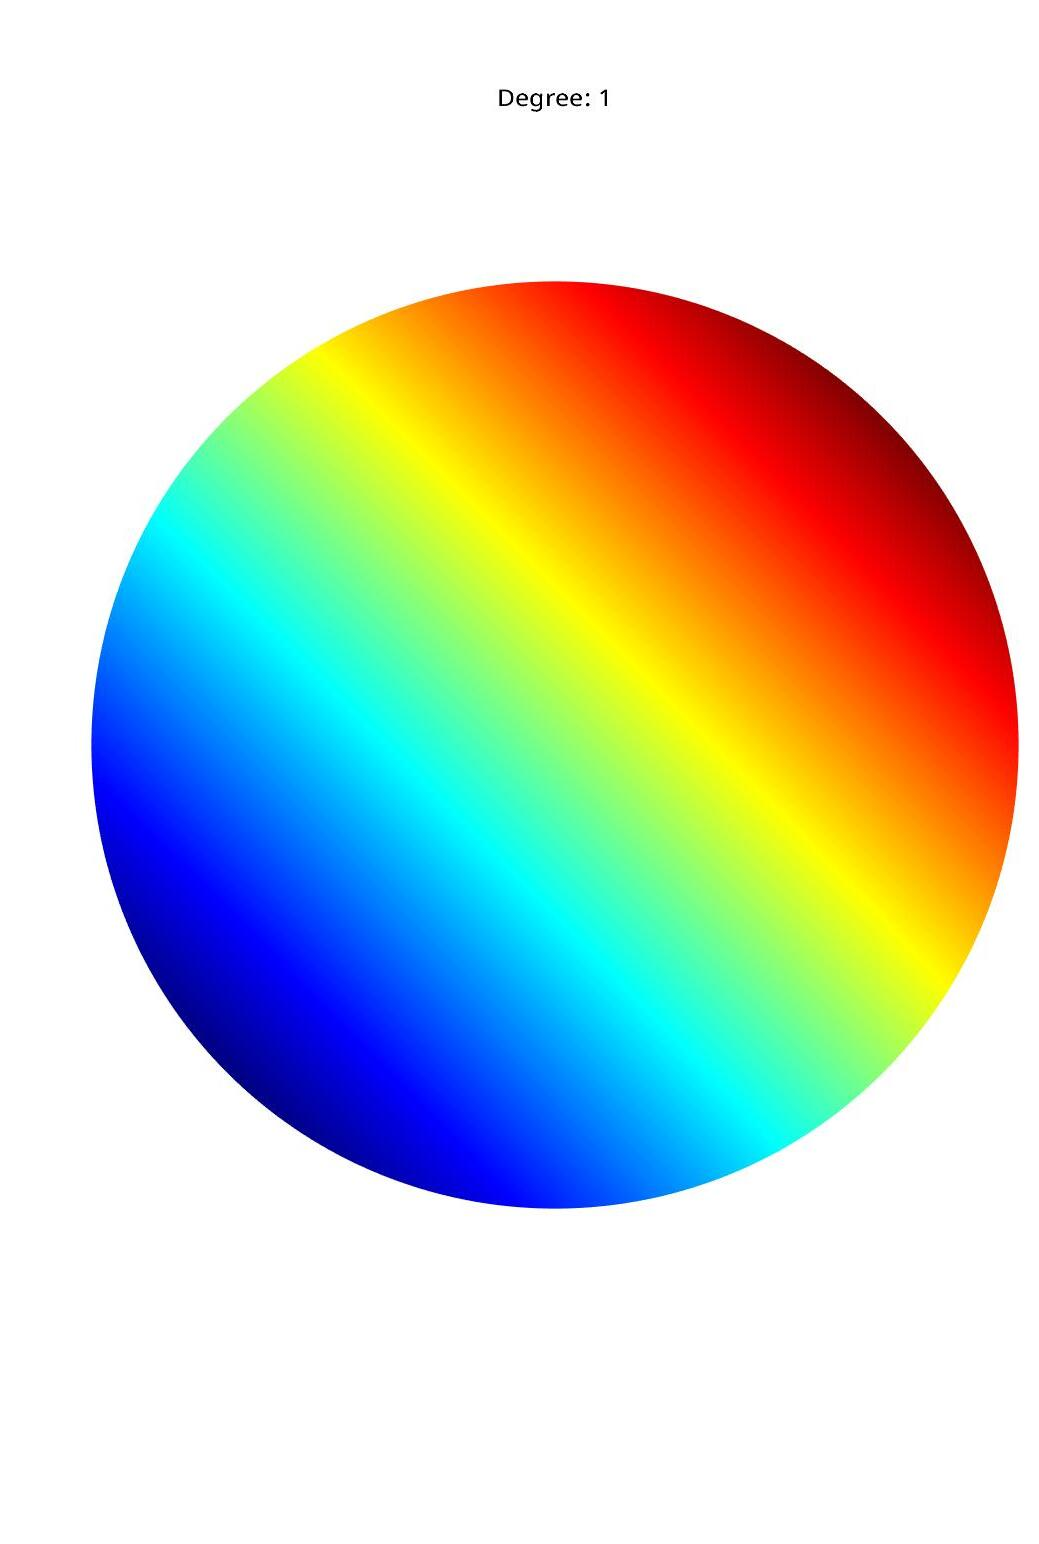
\includegraphics[width=0.95\linewidth]{media/med_1.jpg}
        \label{fig:med1}
    \end{minipage}
    \begin{minipage}{.245\textwidth}
        \centering
        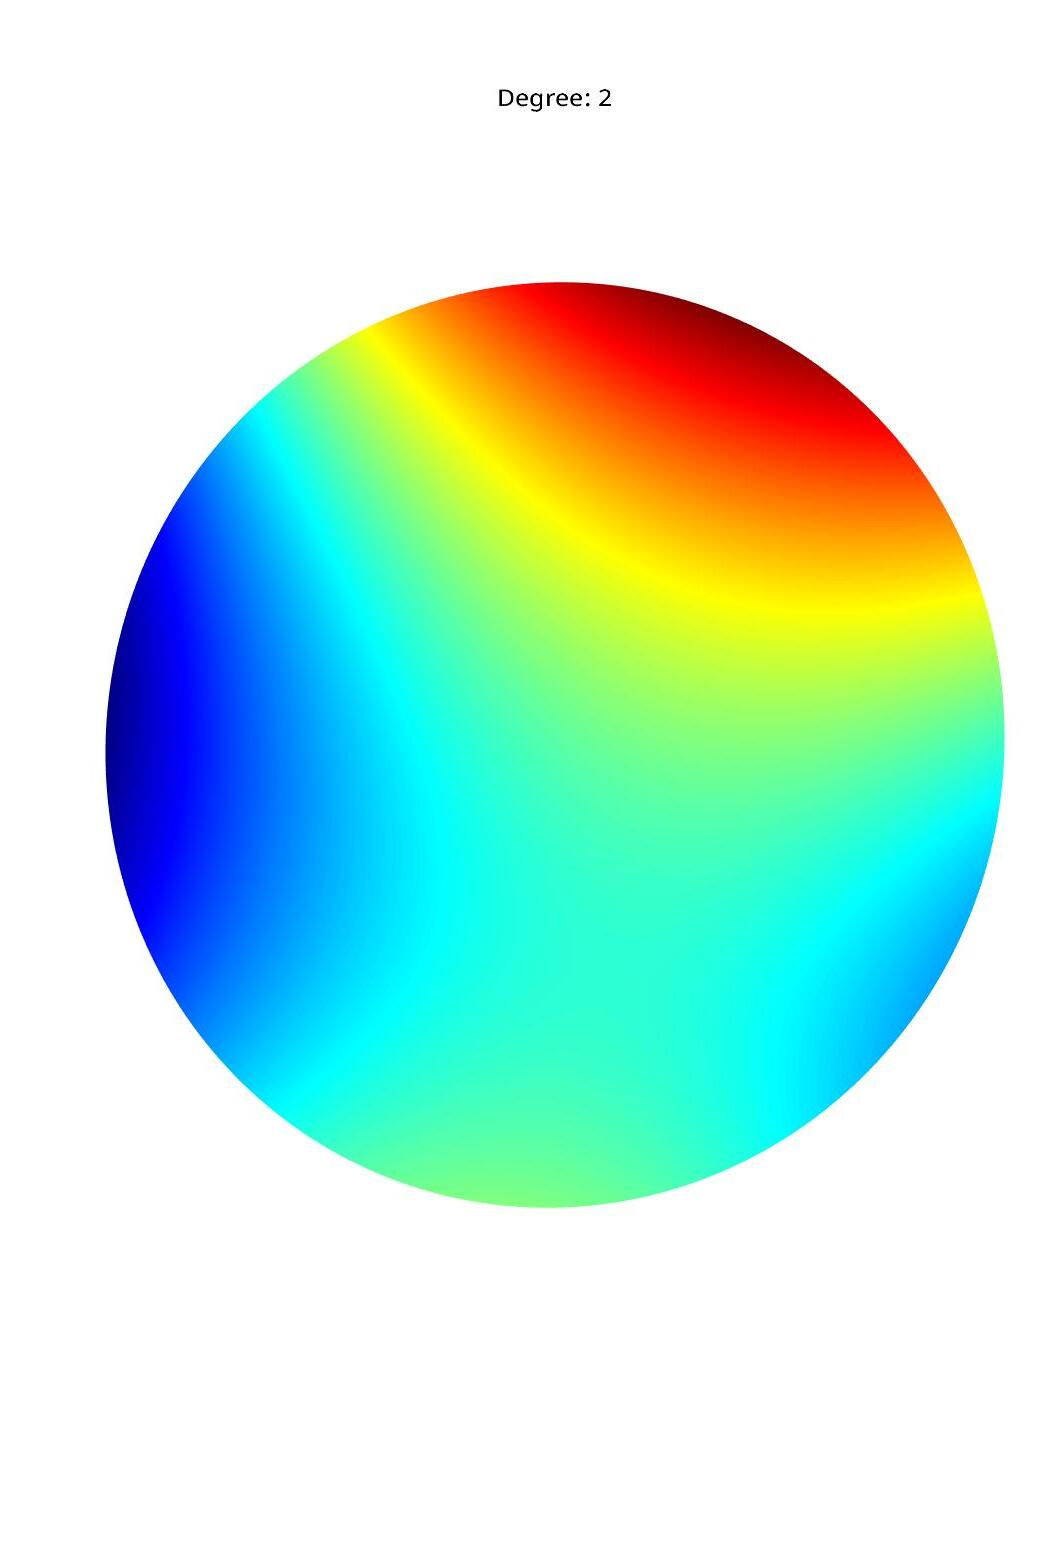
\includegraphics[width=0.95\linewidth]{media/med_2.jpg}
        \label{fig:med2}
    \end{minipage}
    \begin{minipage}{.245\textwidth}
        \centering
        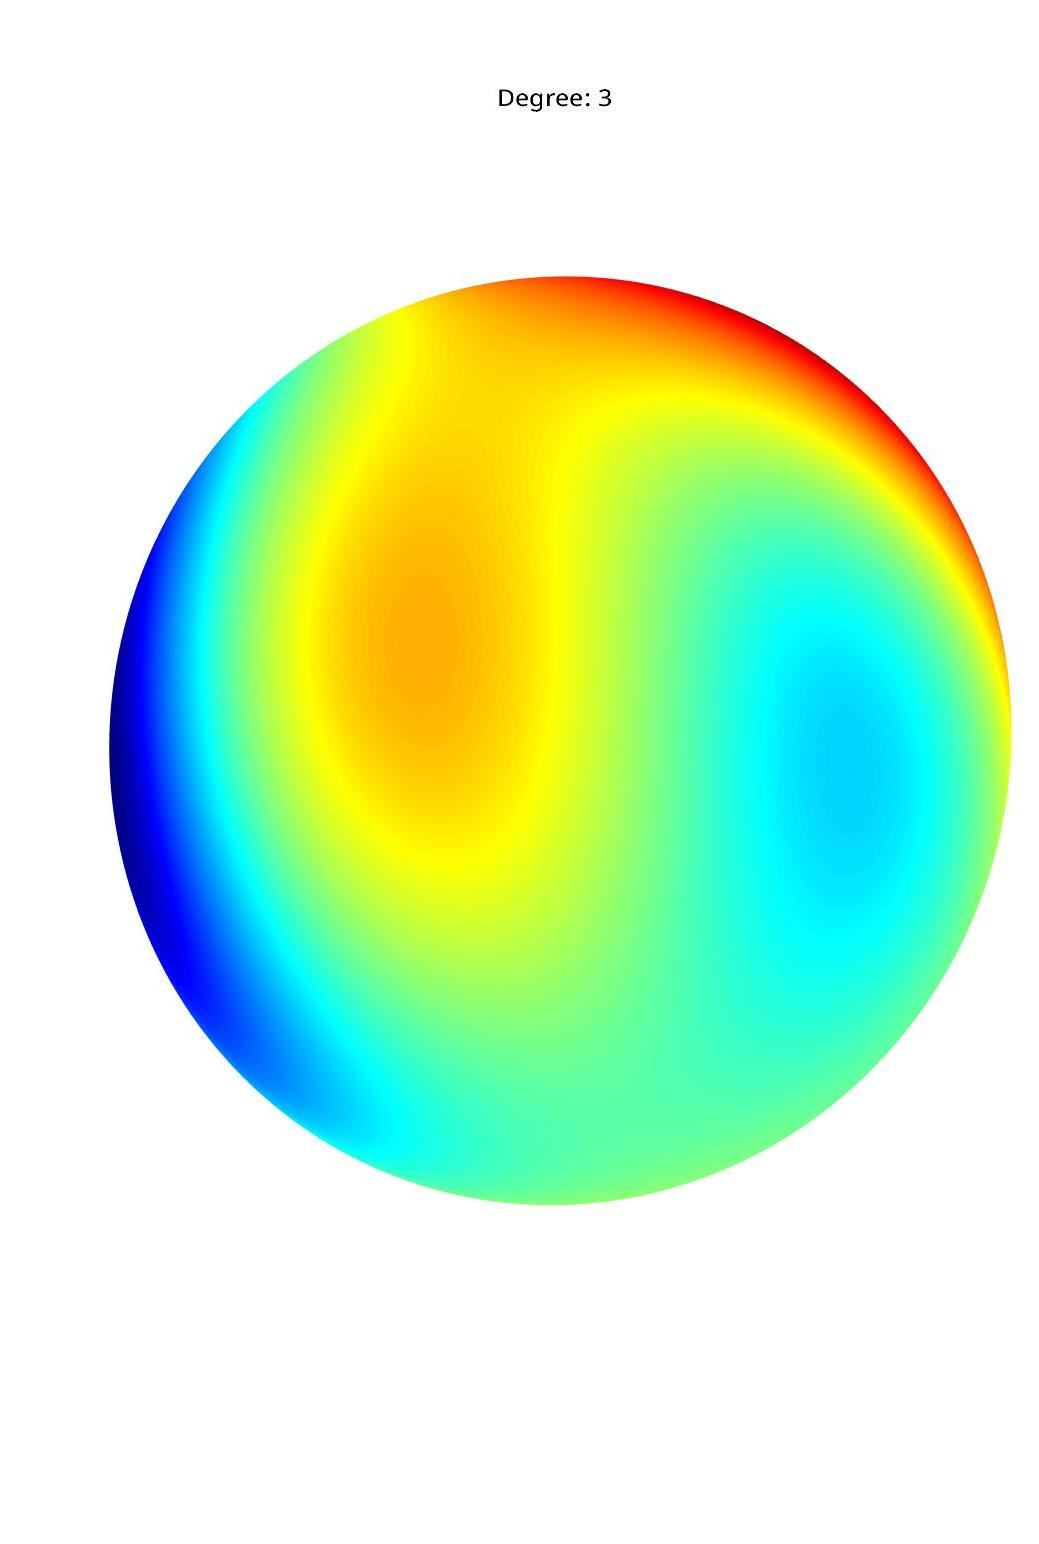
\includegraphics[width=0.95\linewidth]{media/med_3.jpg}
        \label{fig:med3}
    \end{minipage}
    \begin{minipage}{.245\textwidth}
        \centering
        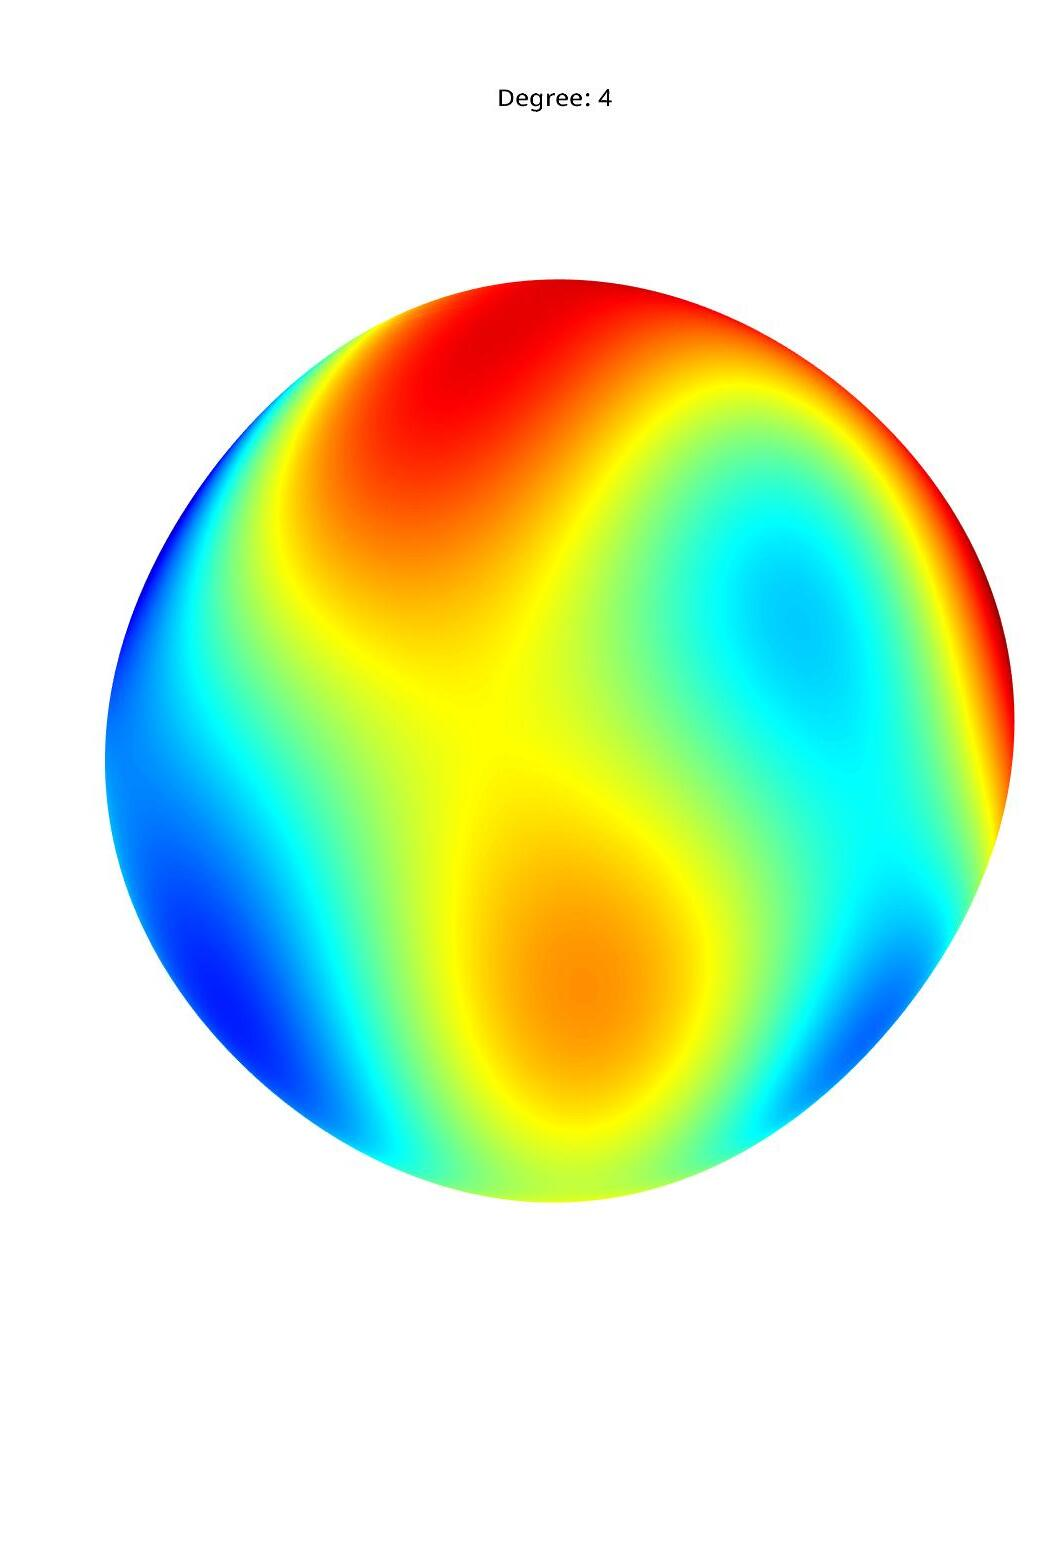
\includegraphics[width=0.95\linewidth]{media/med_4.jpg}
        \label{fig:med4}
    \end{minipage}
    \begin{minipage}{.245\textwidth}
        \centering
        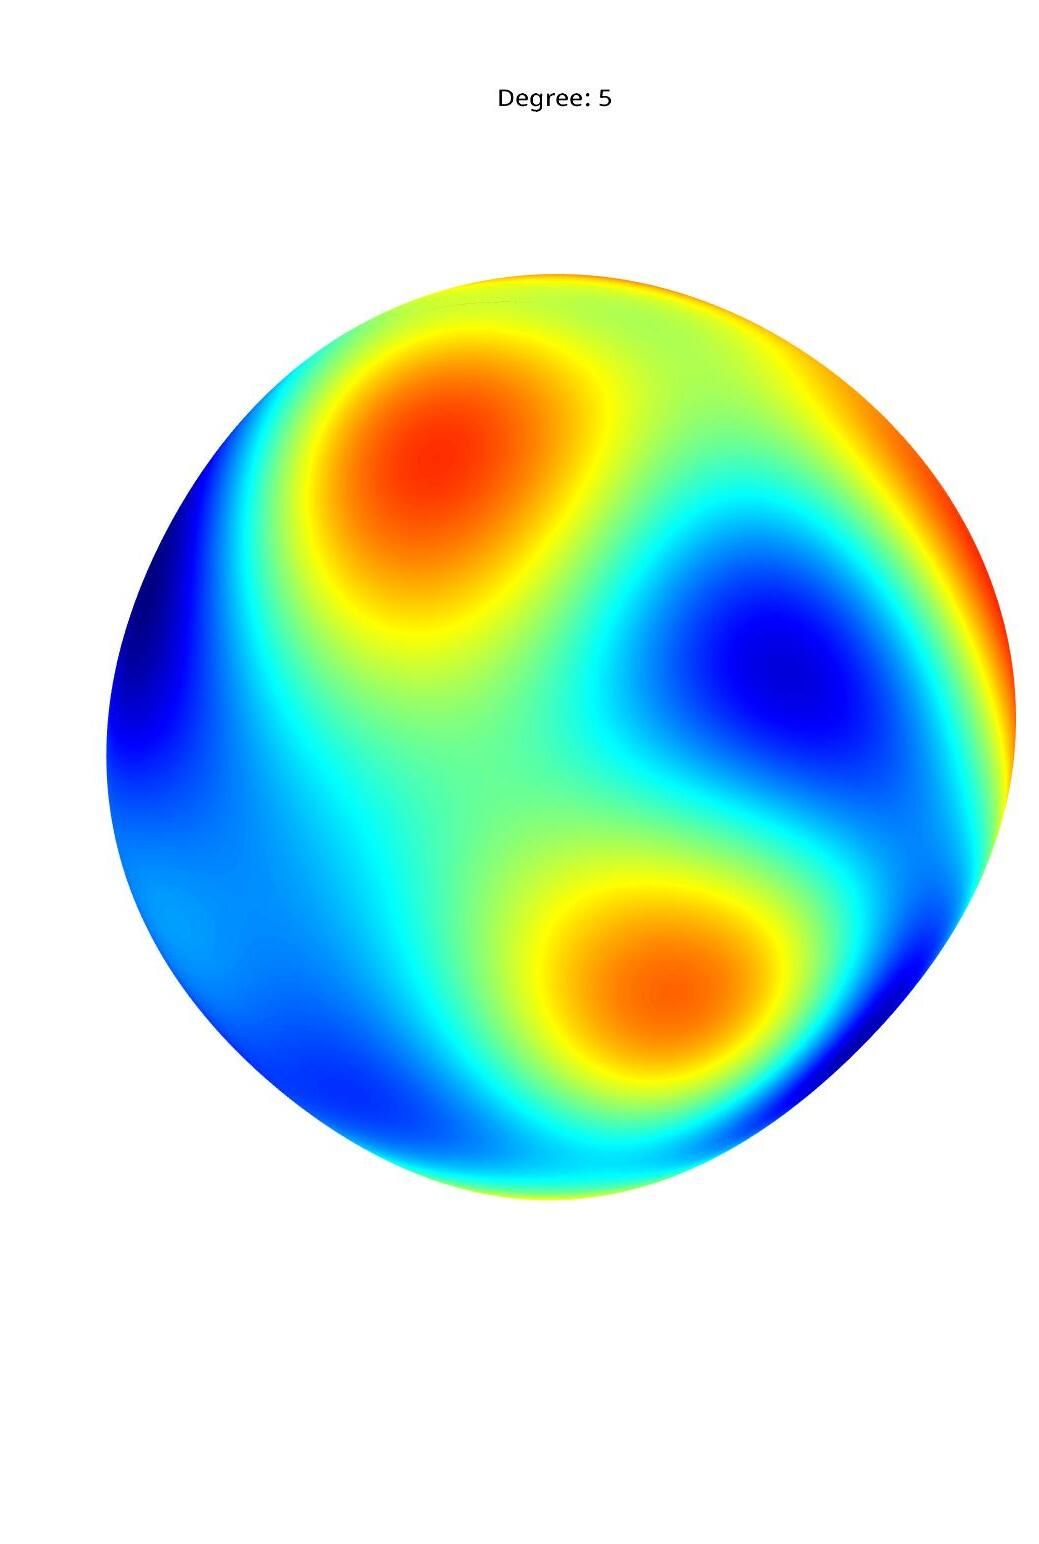
\includegraphics[width=0.95\linewidth]{media/med_5.jpg}
        \label{fig:med5}
    \end{minipage}
    \begin{minipage}{.245\textwidth}
        \centering
        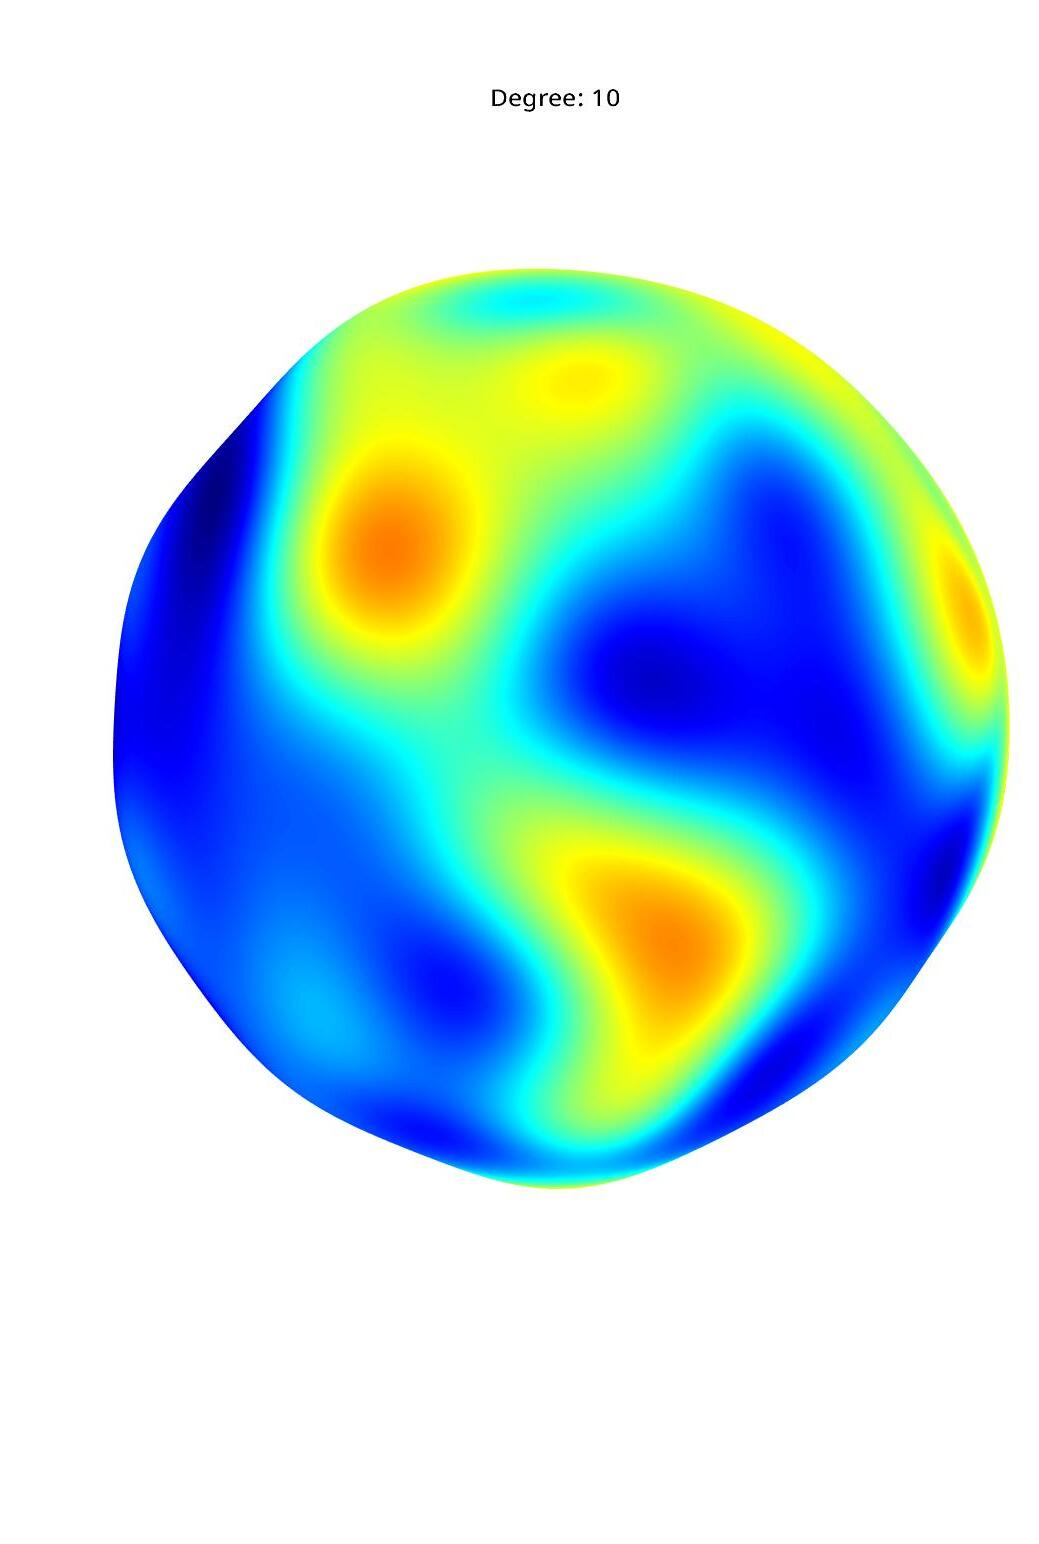
\includegraphics[width=0.95\linewidth]{media/med_10.jpg}
        \label{fig:med10}
    \end{minipage}
    \begin{minipage}{.245\textwidth}
        \centering
        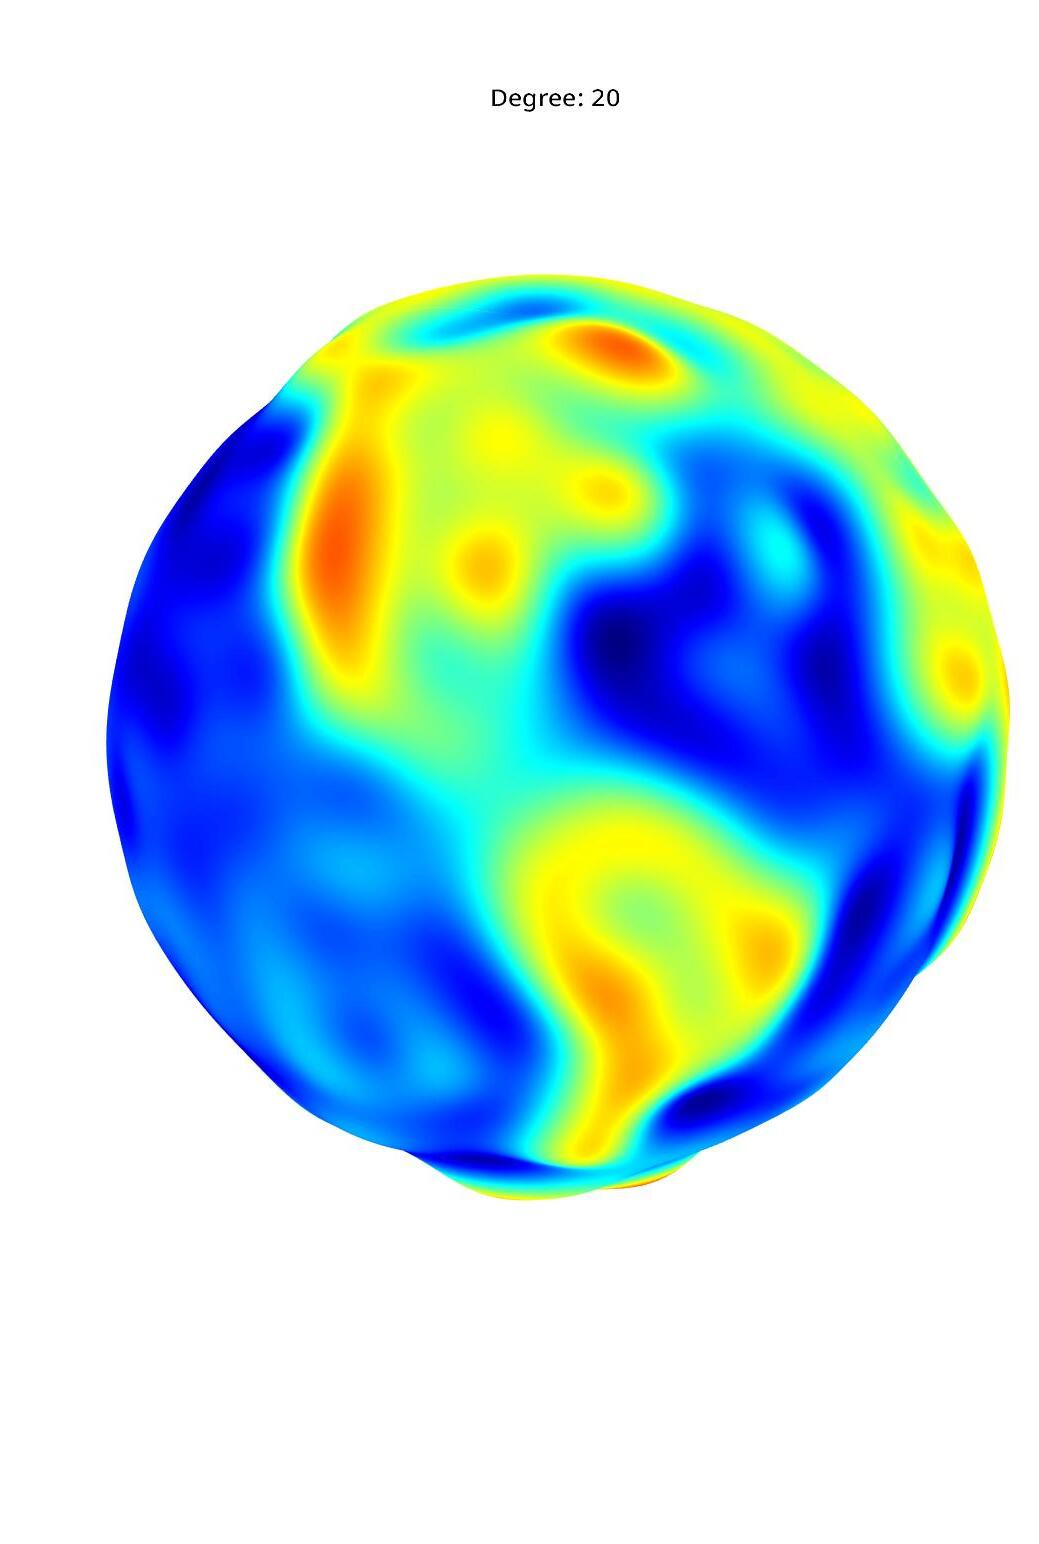
\includegraphics[width=0.95\linewidth]{media/med_20.jpg}
        \label{fig:med20}
    \end{minipage}
    \begin{minipage}{.245\textwidth}
        \centering
        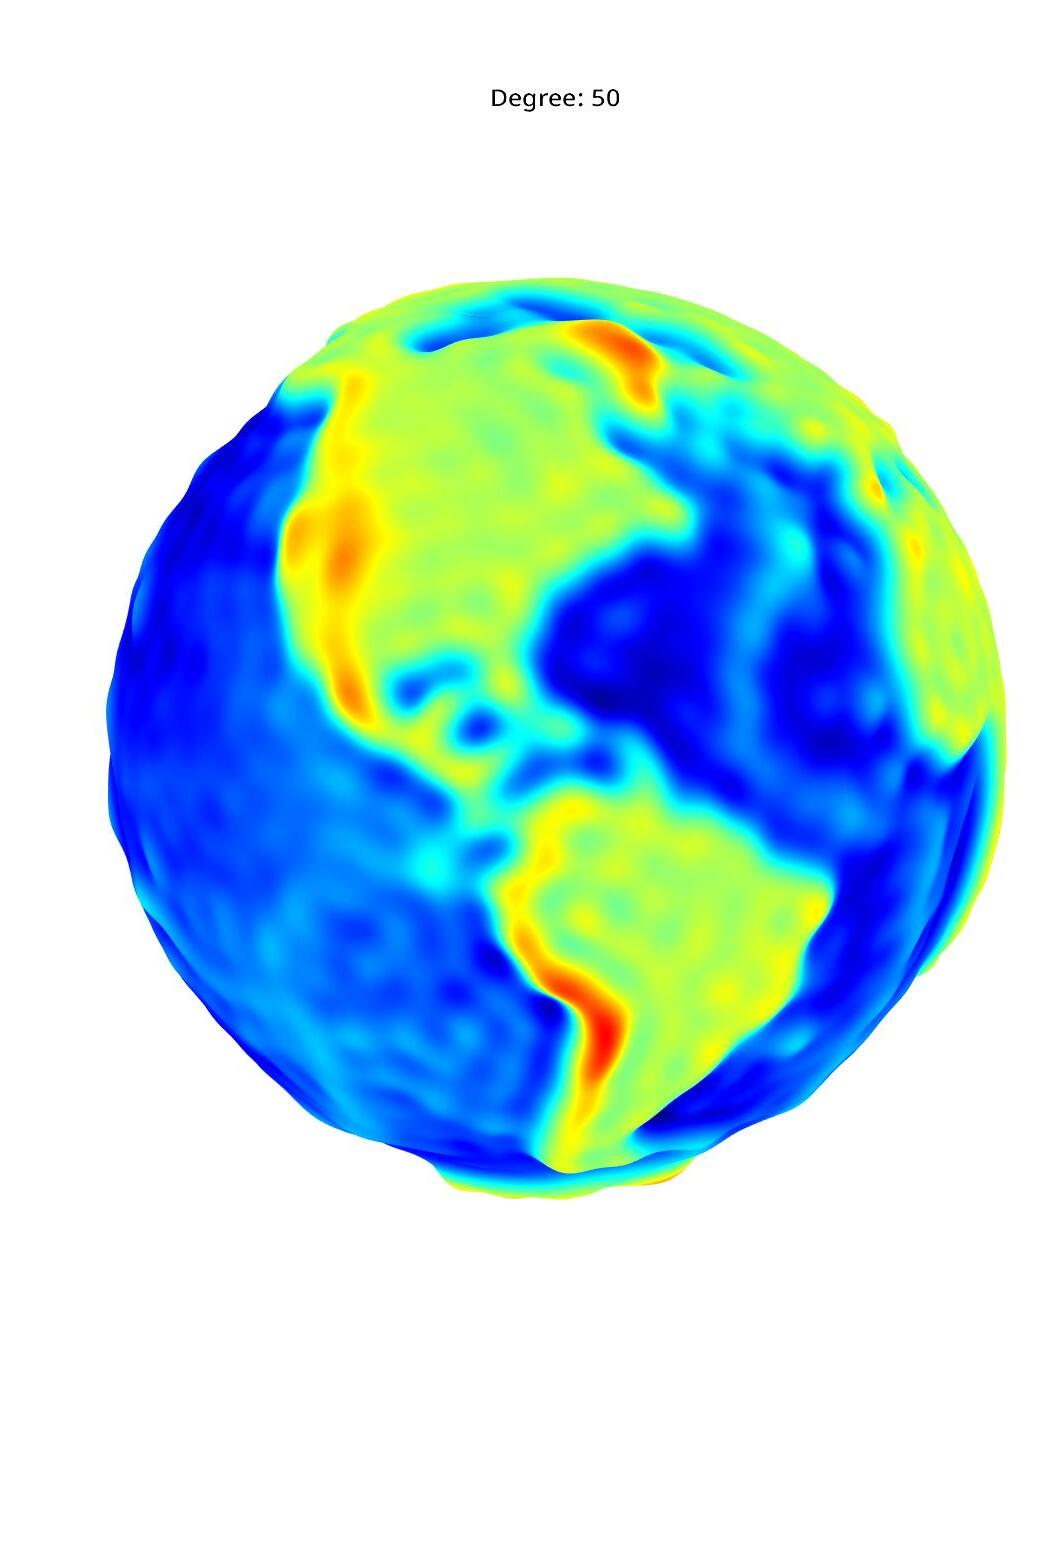
\includegraphics[width=0.95\linewidth]{media/med_50.jpg}
        \label{fig:med50}
    \end{minipage}
    \begin{minipage}{.245\textwidth}
        \centering
        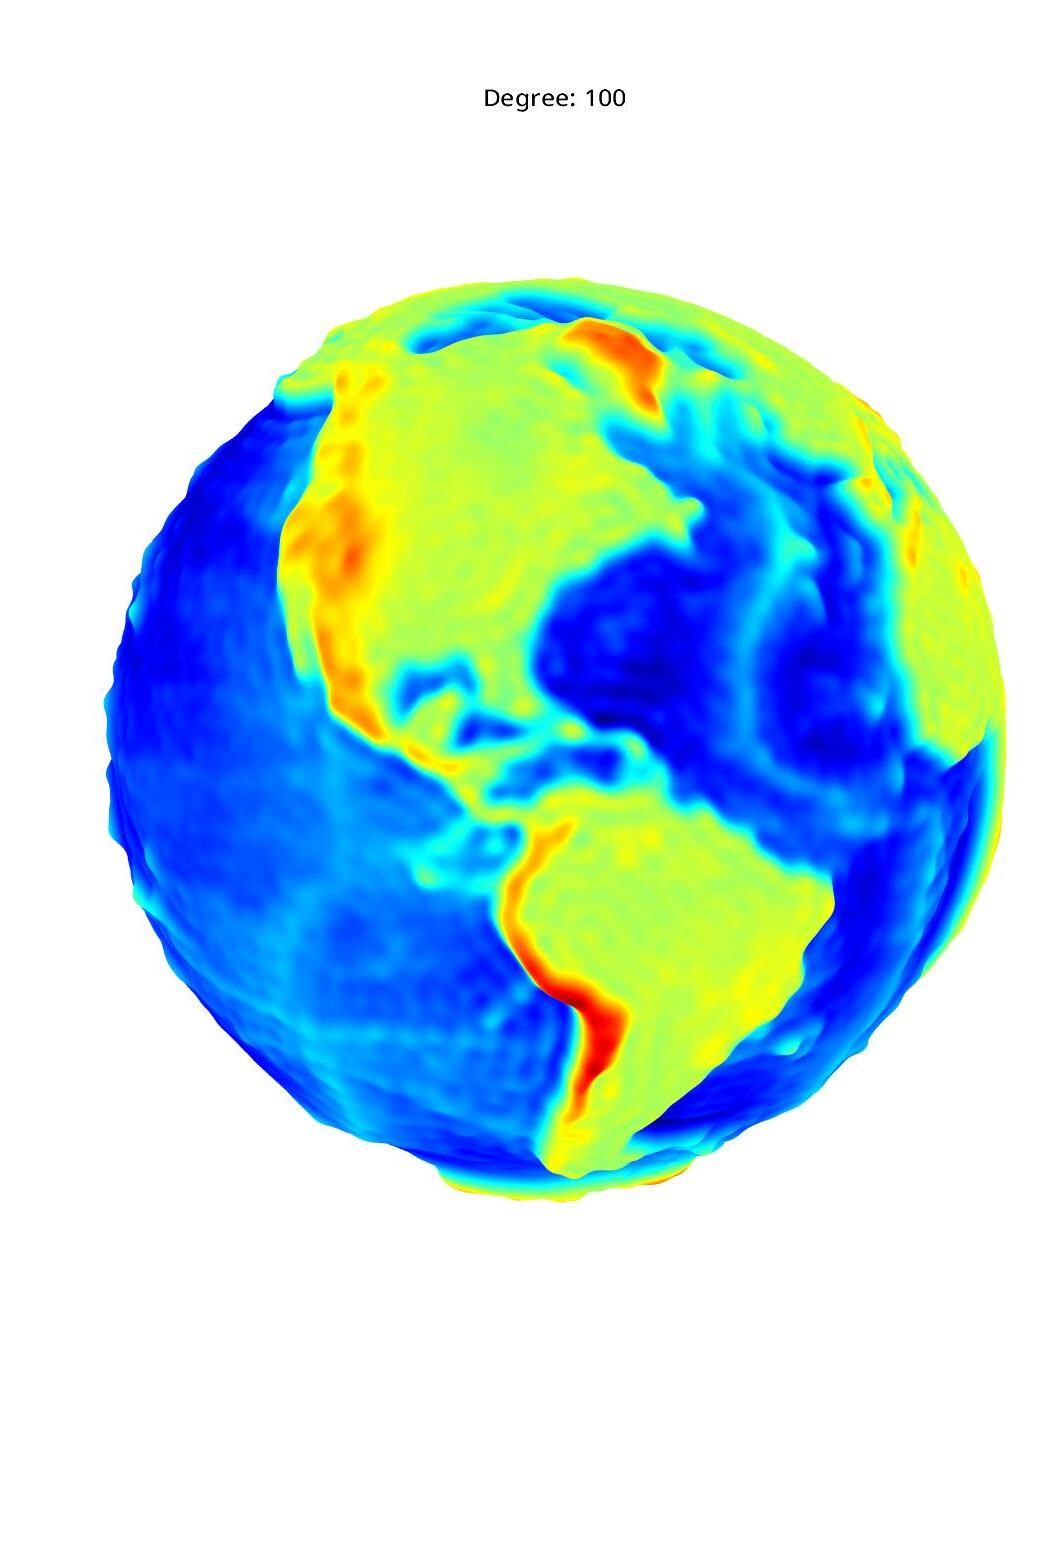
\includegraphics[width=0.95\linewidth]{media/med_100.jpg}
        \label{fig:med100}
    \end{minipage}
    \begin{minipage}{.245\textwidth}
        \centering
        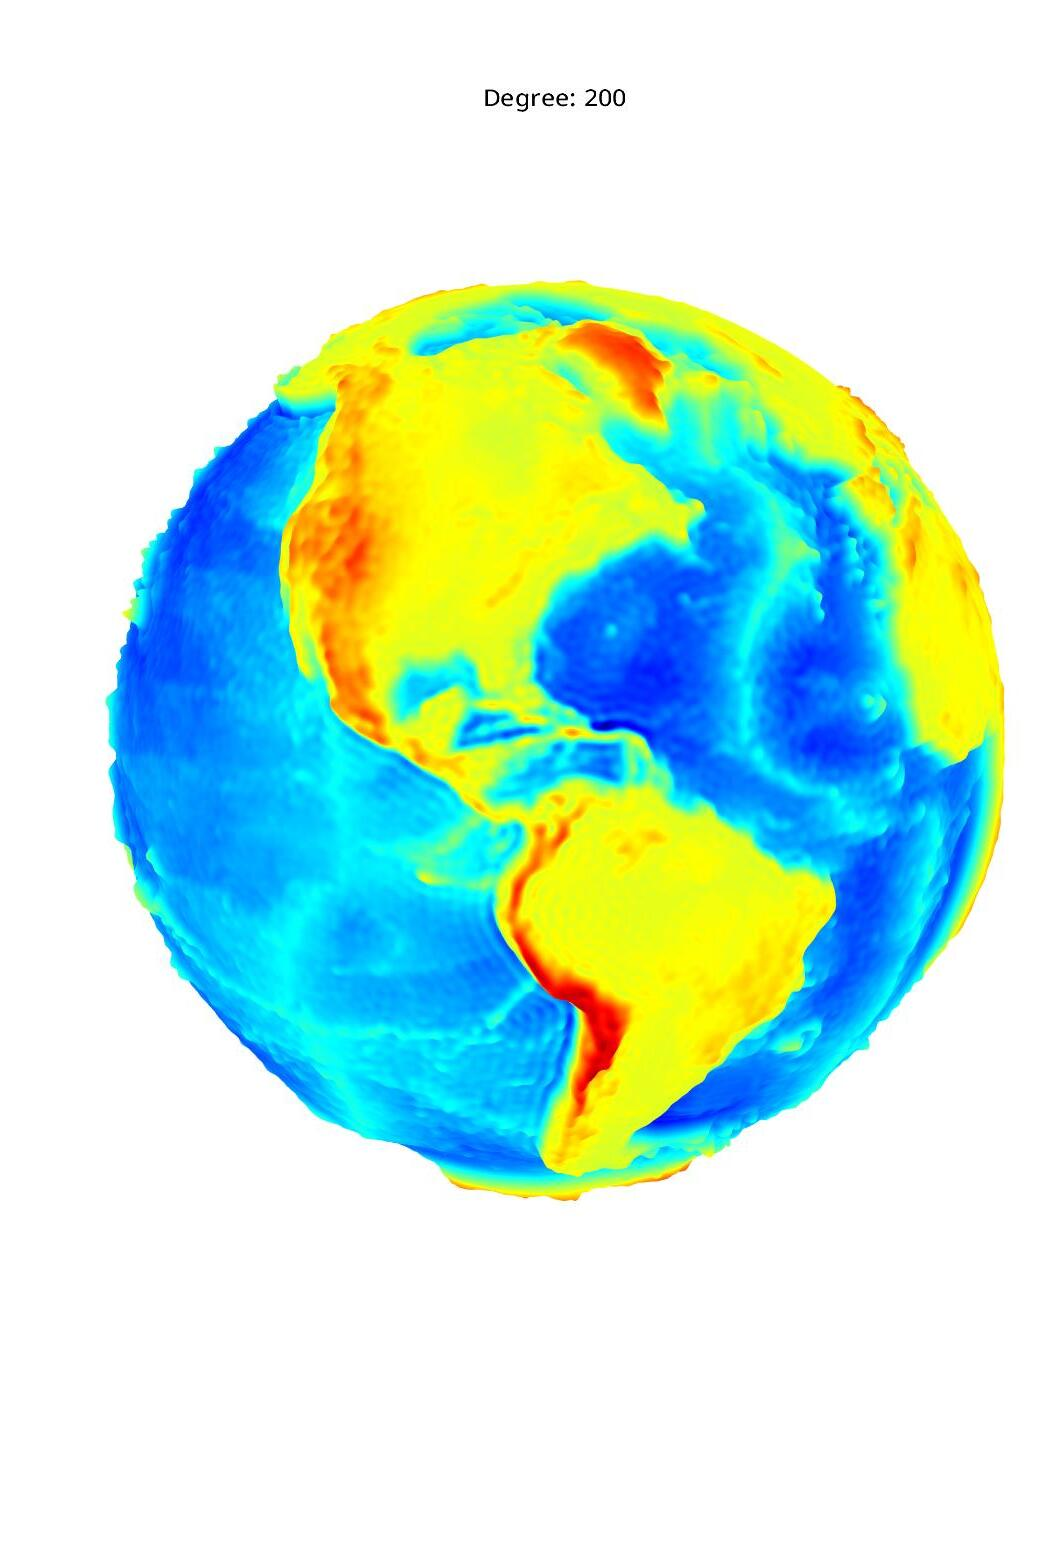
\includegraphics[width=0.95\linewidth]{media/med_200.jpg}
        \label{fig:med200}
    \end{minipage}
    \begin{minipage}{.245\textwidth}
        \centering
        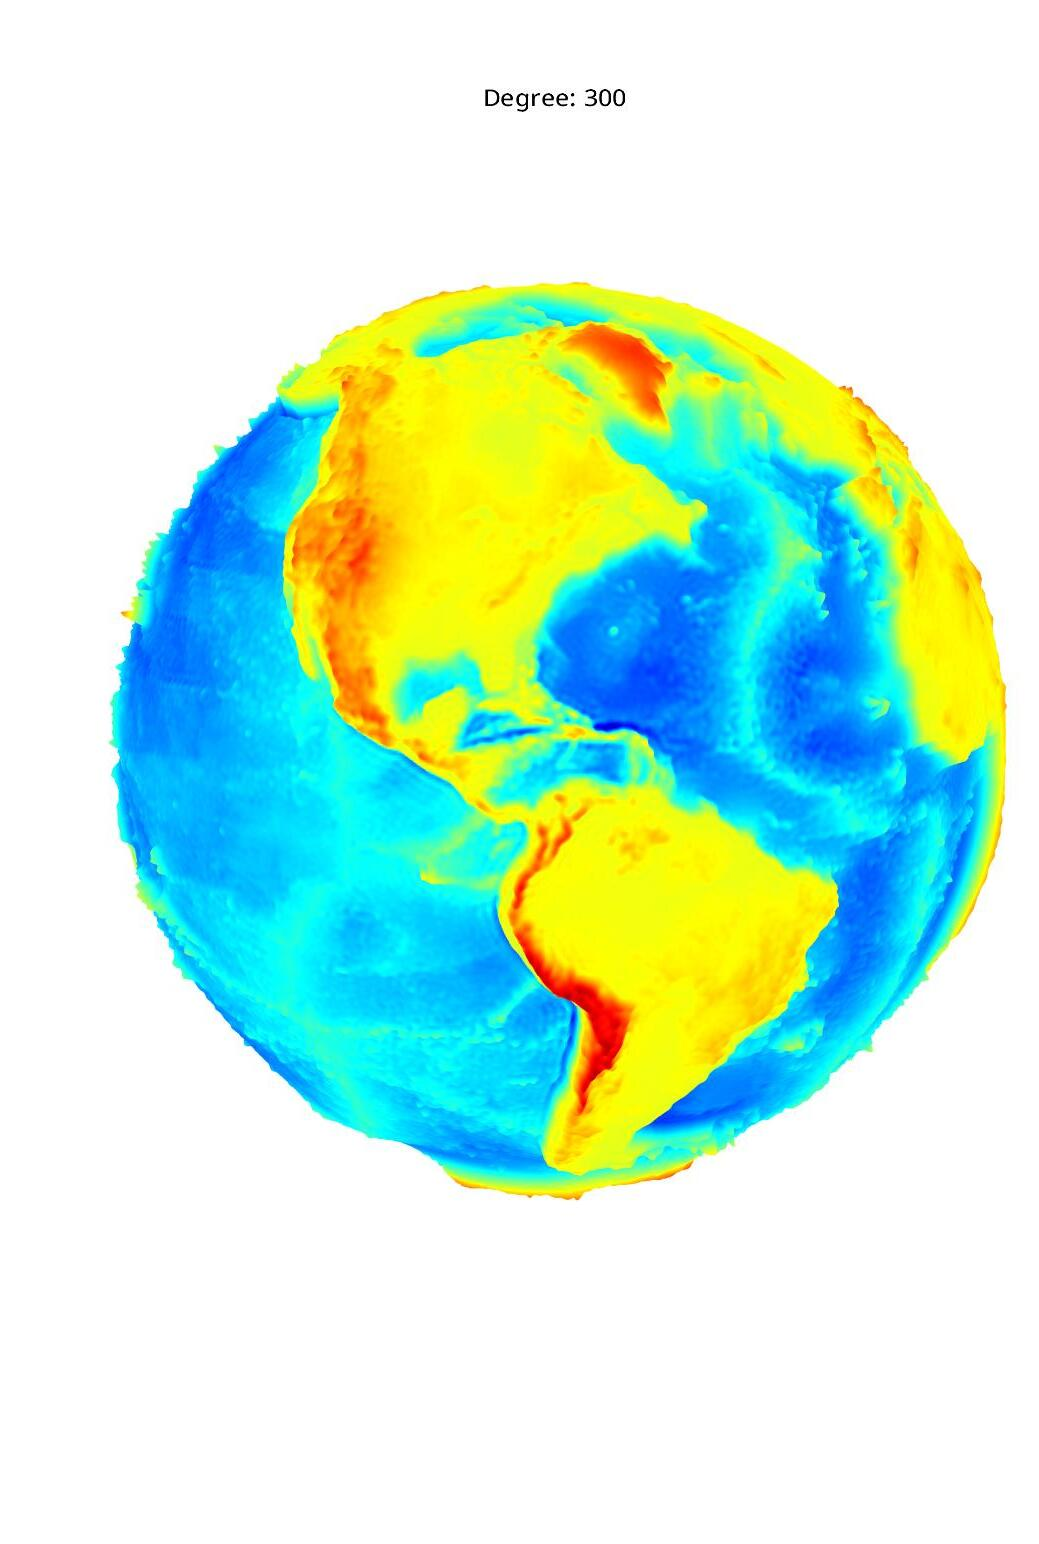
\includegraphics[width=0.95\linewidth]{media/med_300.jpg}
        \label{fig:med300}
    \end{minipage}
    \begin{minipage}{.245\textwidth}
        \centering
        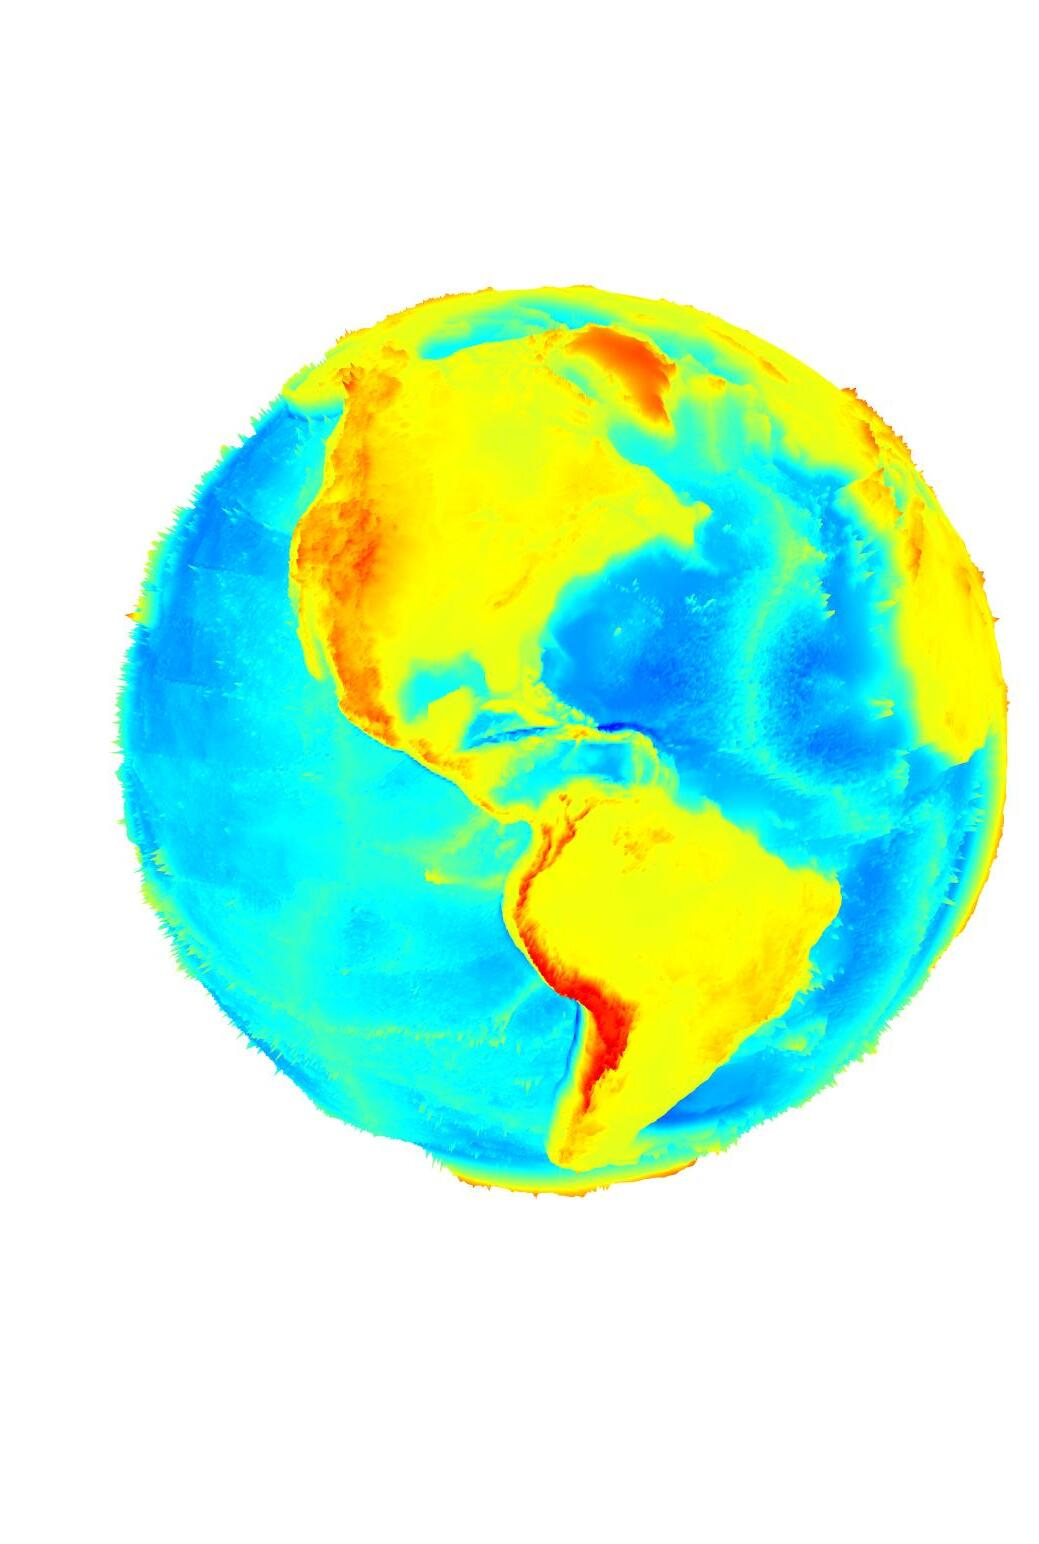
\includegraphics[width=0.95\linewidth]{media/med.jpg}
        \label{fig:med}
    \end{minipage}
    \caption{Altitude prediction of a model for varying degrees of a model. In the top row we have models of degree $l \in \{1, 2, 3, 4\}$, middle row $l \in \{5, 10, 20, 50\}$, and finally the bottom
    row $l \in \{100, 200, 300, +\infty\}$. The final visualization on the bottom right corresponds to the observed values of $f$.}
    \label{fig:earth_models}
\end{figure}

Evidently, as we increase the degree of the model the difference between the predicted values $\hat f_i$ and the observations $f_i$ will tend to 
shrink in magnitude. Let's take a look at the distributions of $r = \hat f - f$ for models of degree up to $l = 300$.

Recall to a simpler time where we computed models of degree $l = 20$. Refer to Figure \ref{fig:error} to verify that the average absolute error sits at around 
600 for a model of the small data with coefficients going up to $l = 20$. Now consider the following distributions of the errors of models built on the small data set
with degrees up to 300.

\begin{figure}[h!]
\begin{minipage}{.45\textwidth}
    \centering
        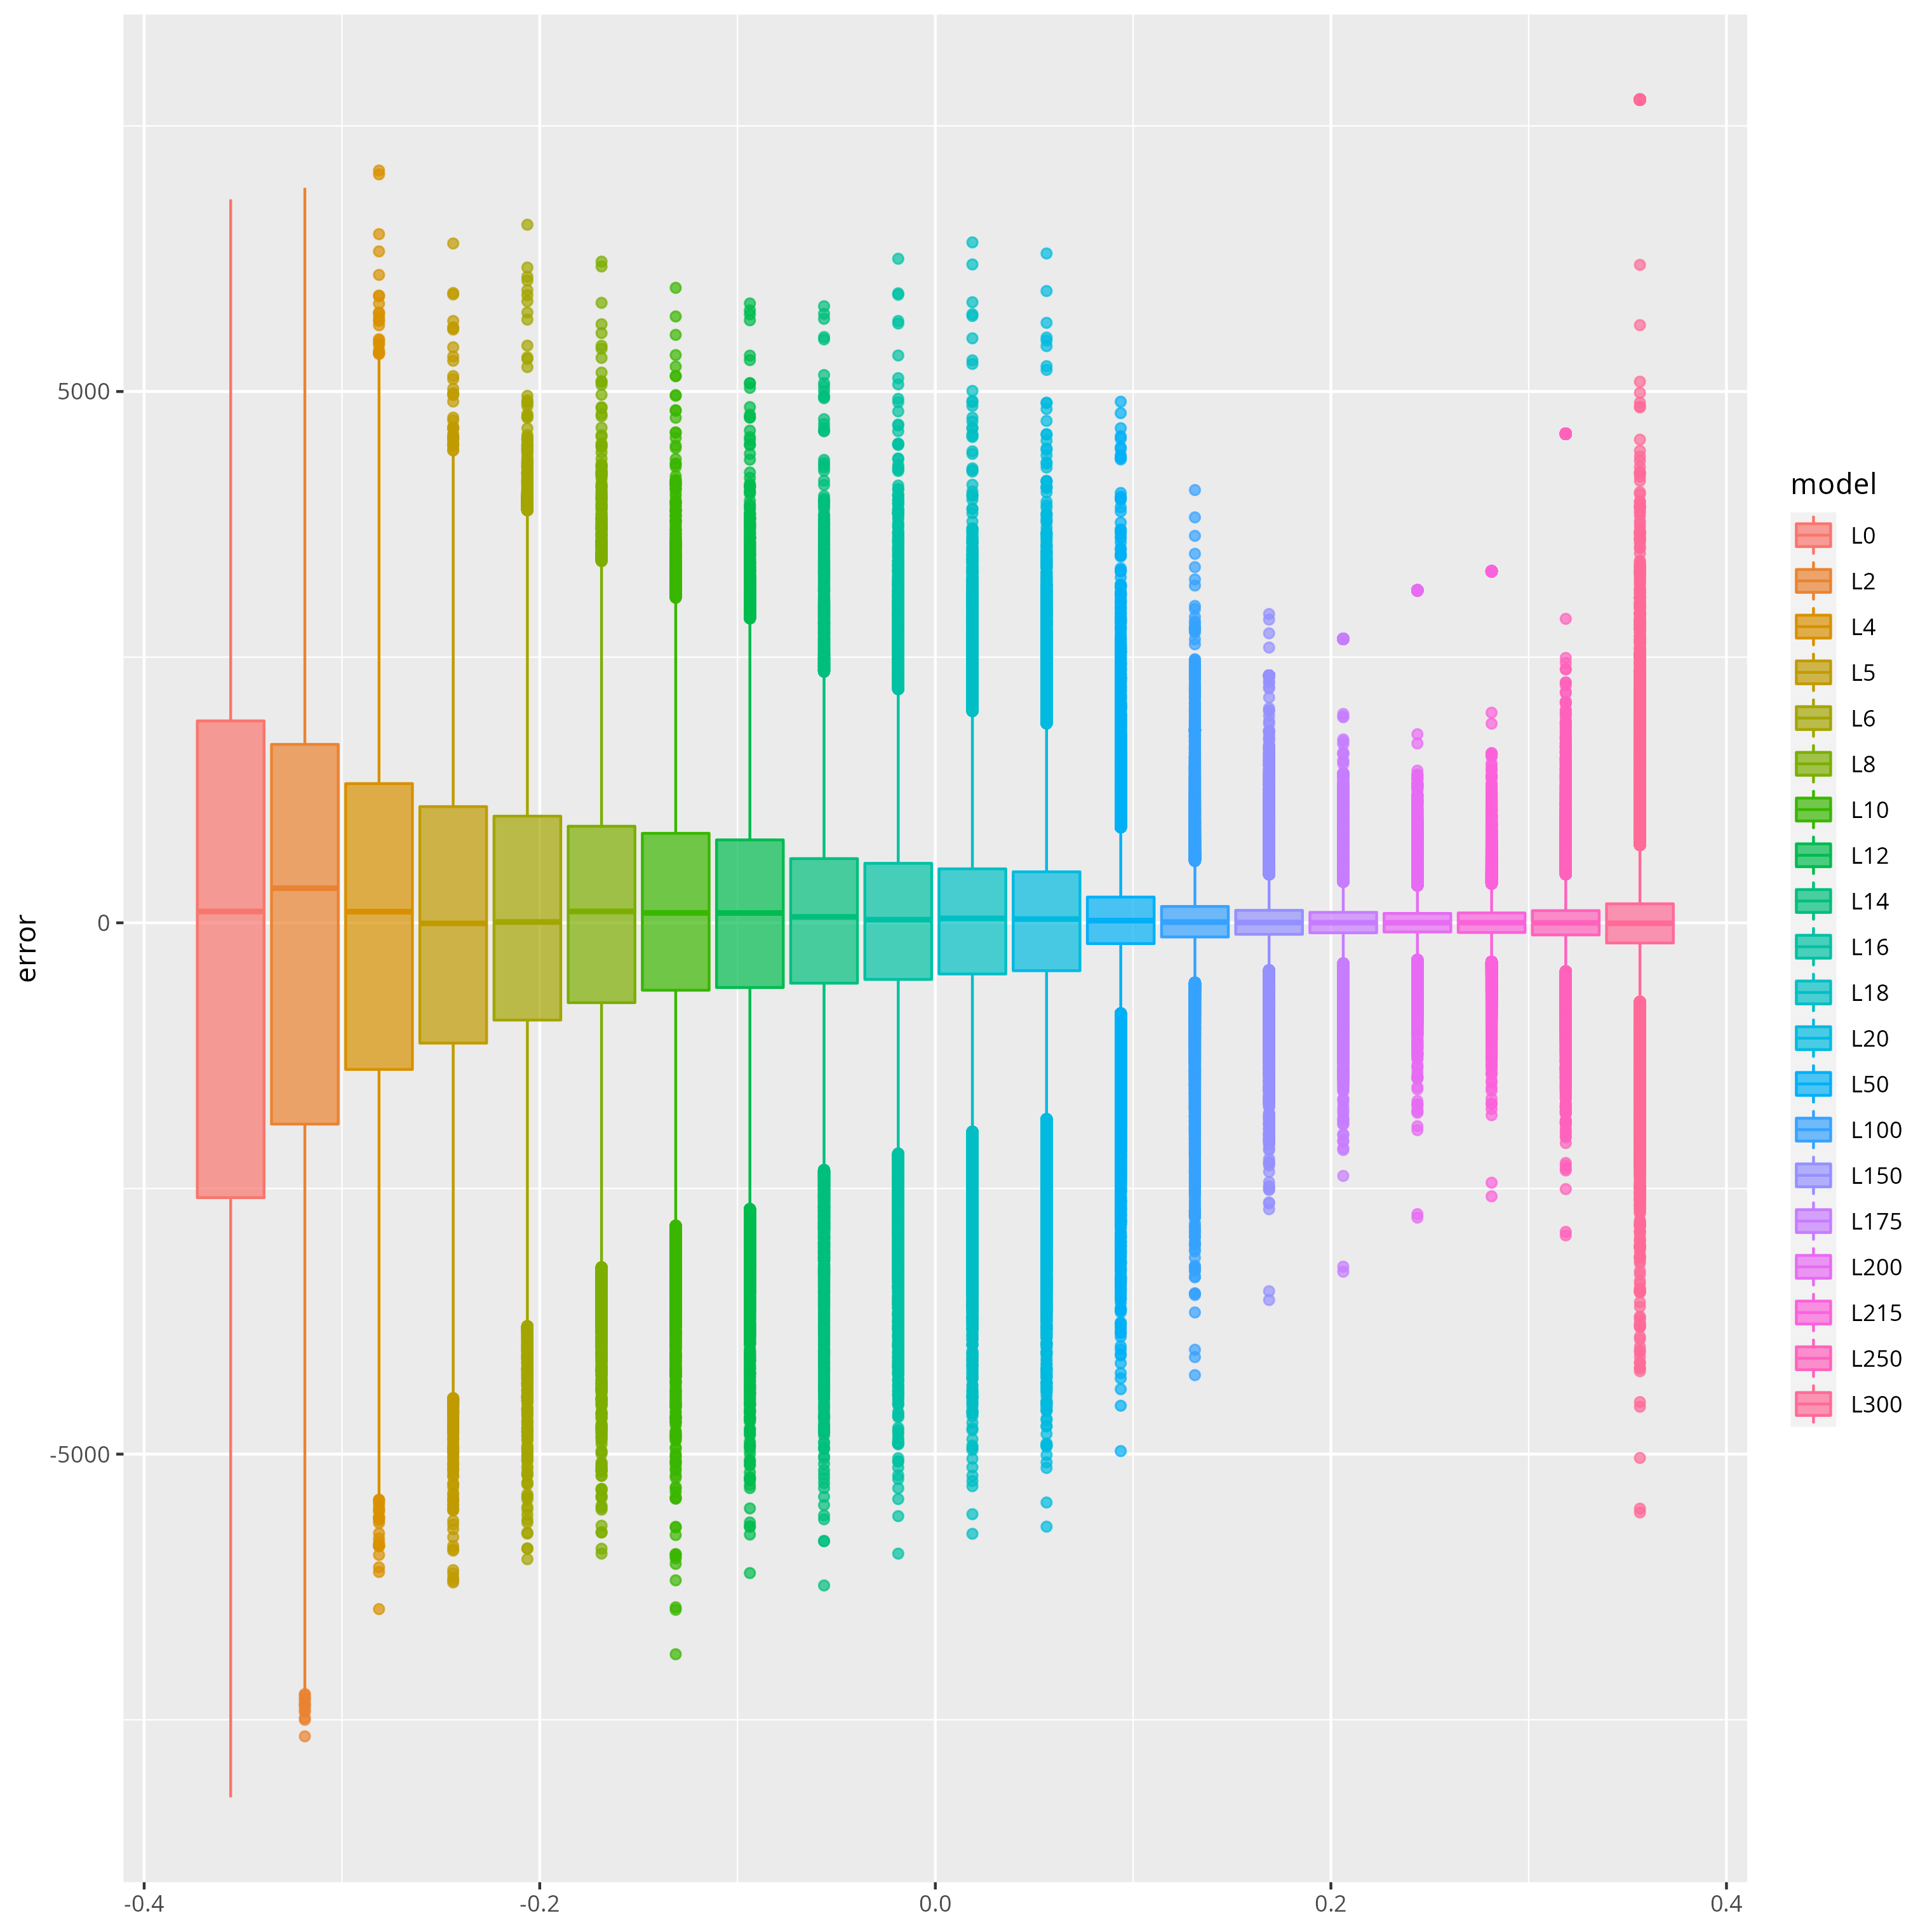
\includegraphics[width=0.9\linewidth]{media/small_error_box.png}
\end{minipage}
\begin{minipage}{.45\textwidth}
    \centering
        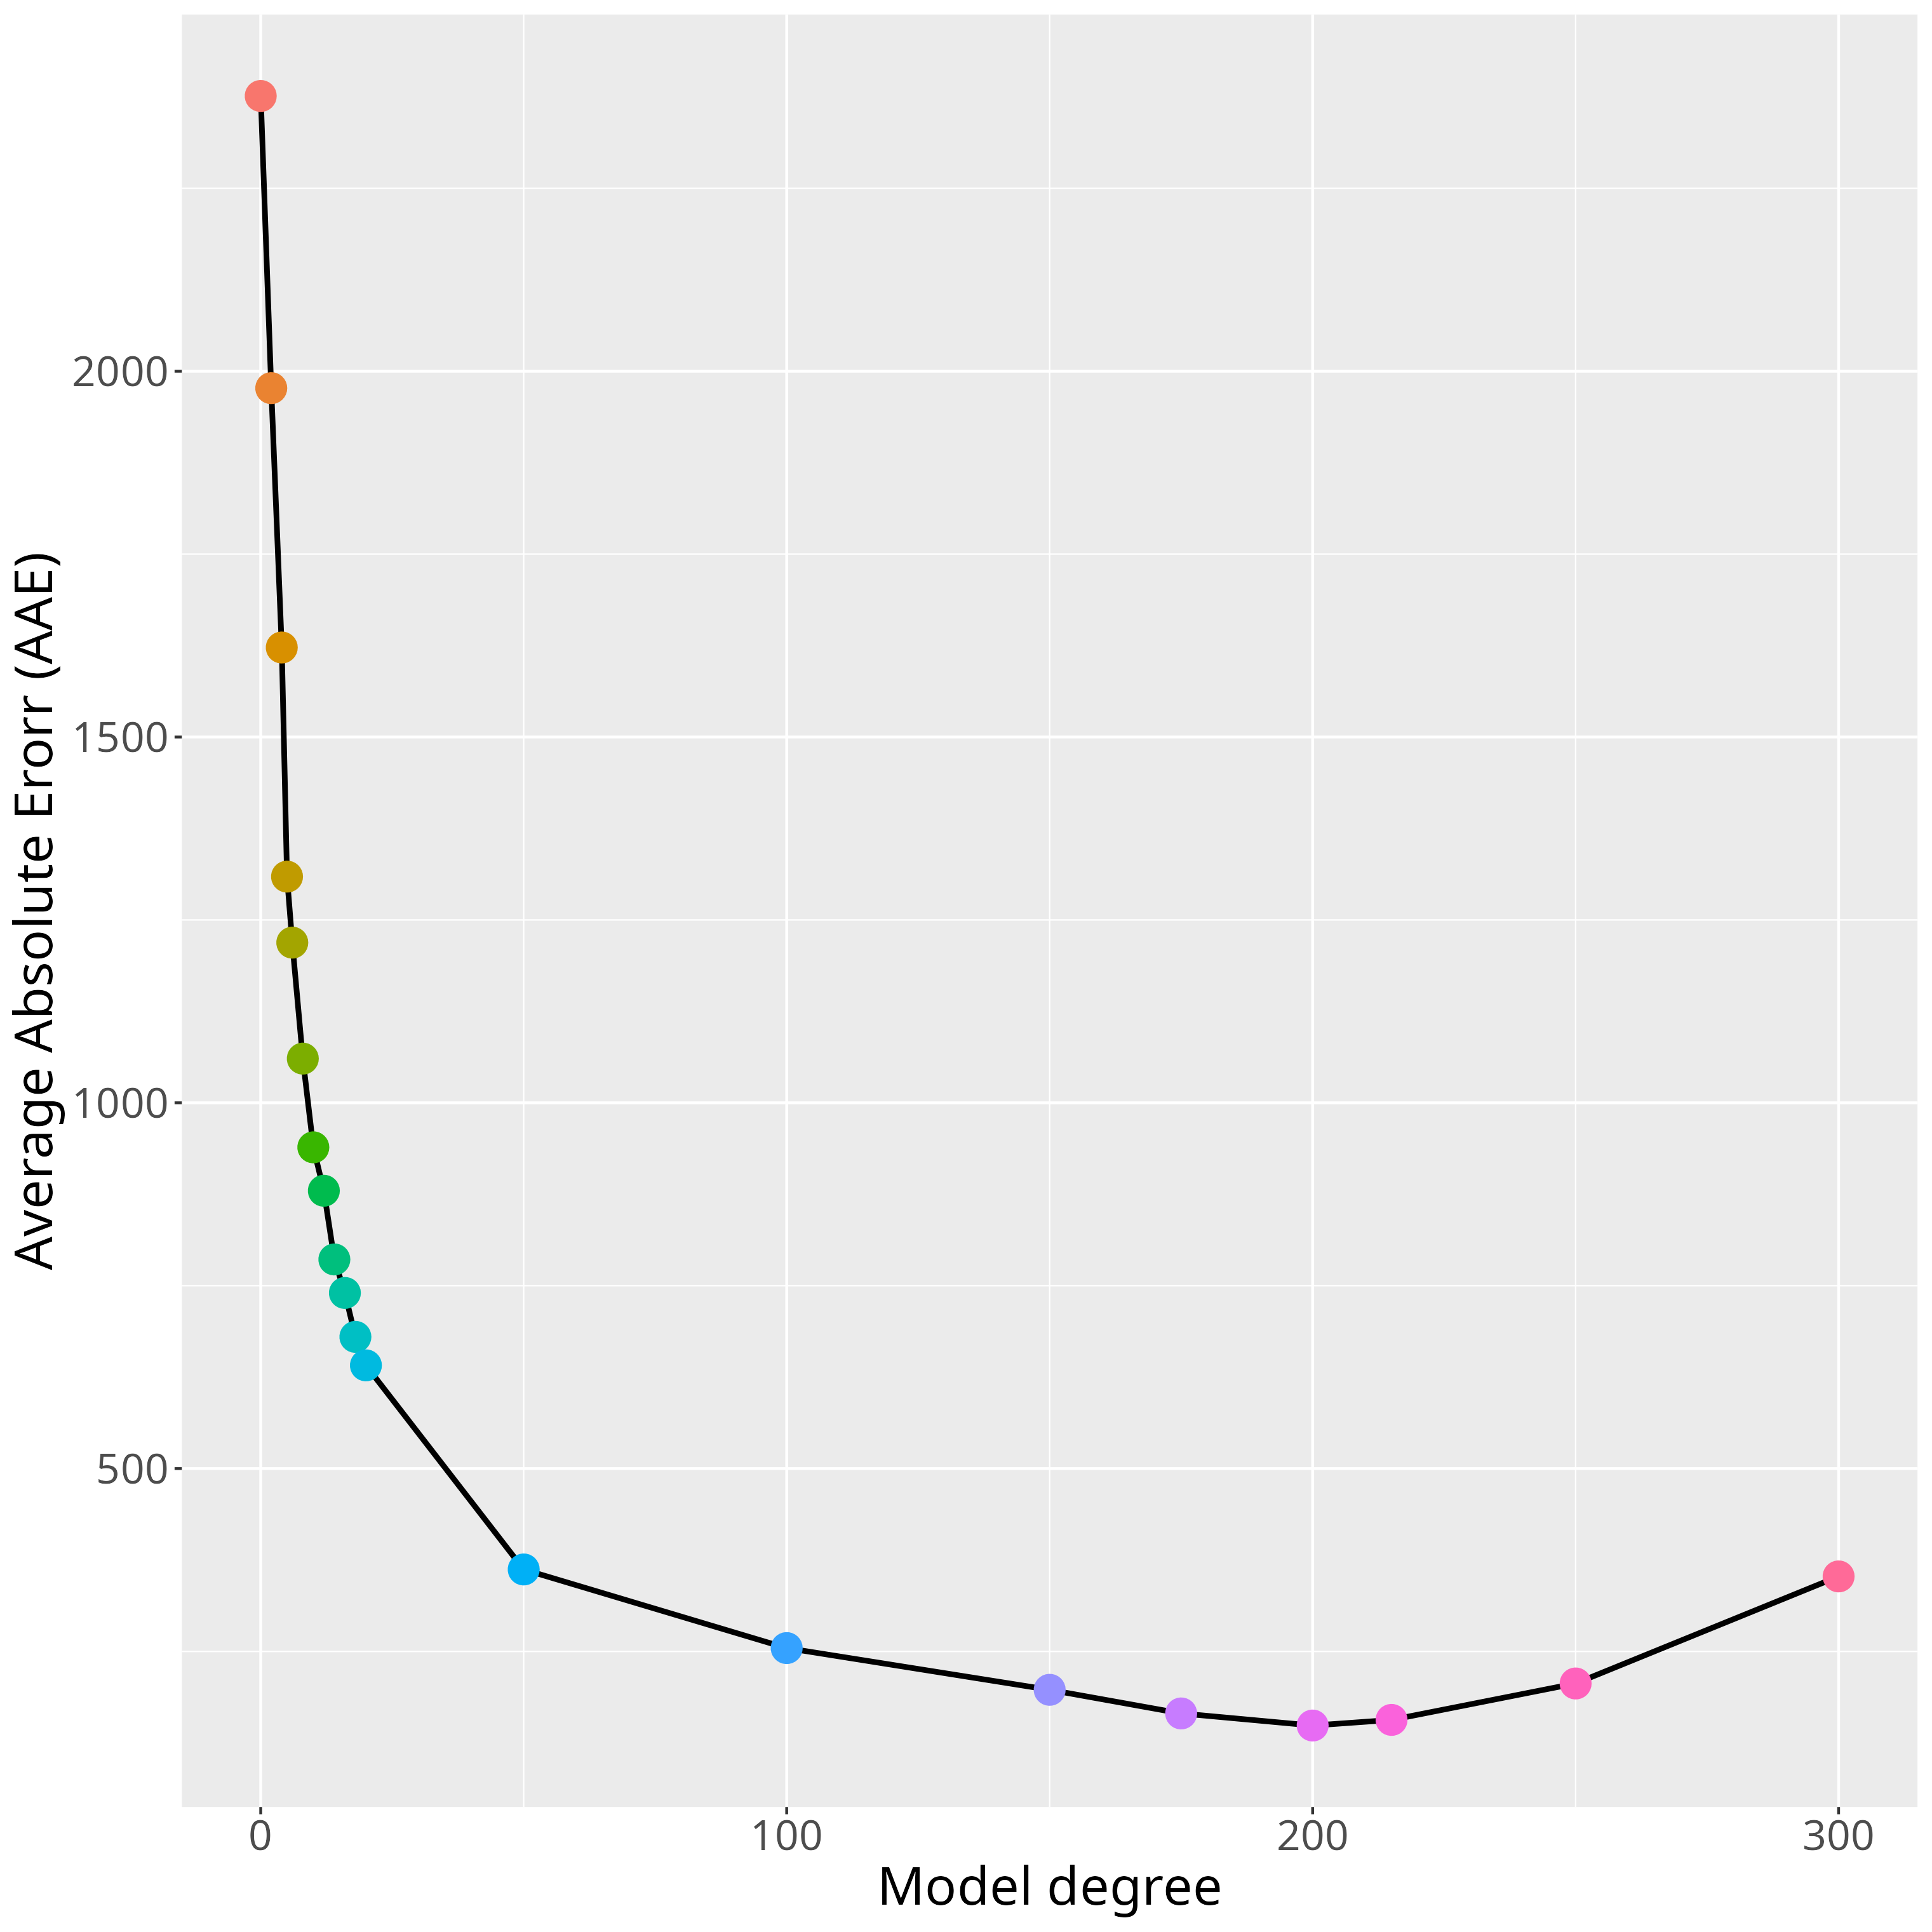
\includegraphics[width=0.9\linewidth]{media/small_err.png}
\end{minipage}
\caption{Boxplot of the residuals $r_i = \hat f_i - f_i$ (left) for models of degree up to $l = 300$ and the AAE associated (right)
built on the small dataset.}
\end{figure}

We notice from these graphs that there seems to be a certain optimal degree of the model, afterwhich the AAE begins to increase.
For the small data set, this optimum sits at just around 200, and we find that the best model for the small data set has an AAE of 
148.7594

We conduct an analagous exploration with the medium data set, this time generating models of up to $l = 800$:

\begin{figure}[h!]
    \begin{minipage}{.45\textwidth}
        \centering
            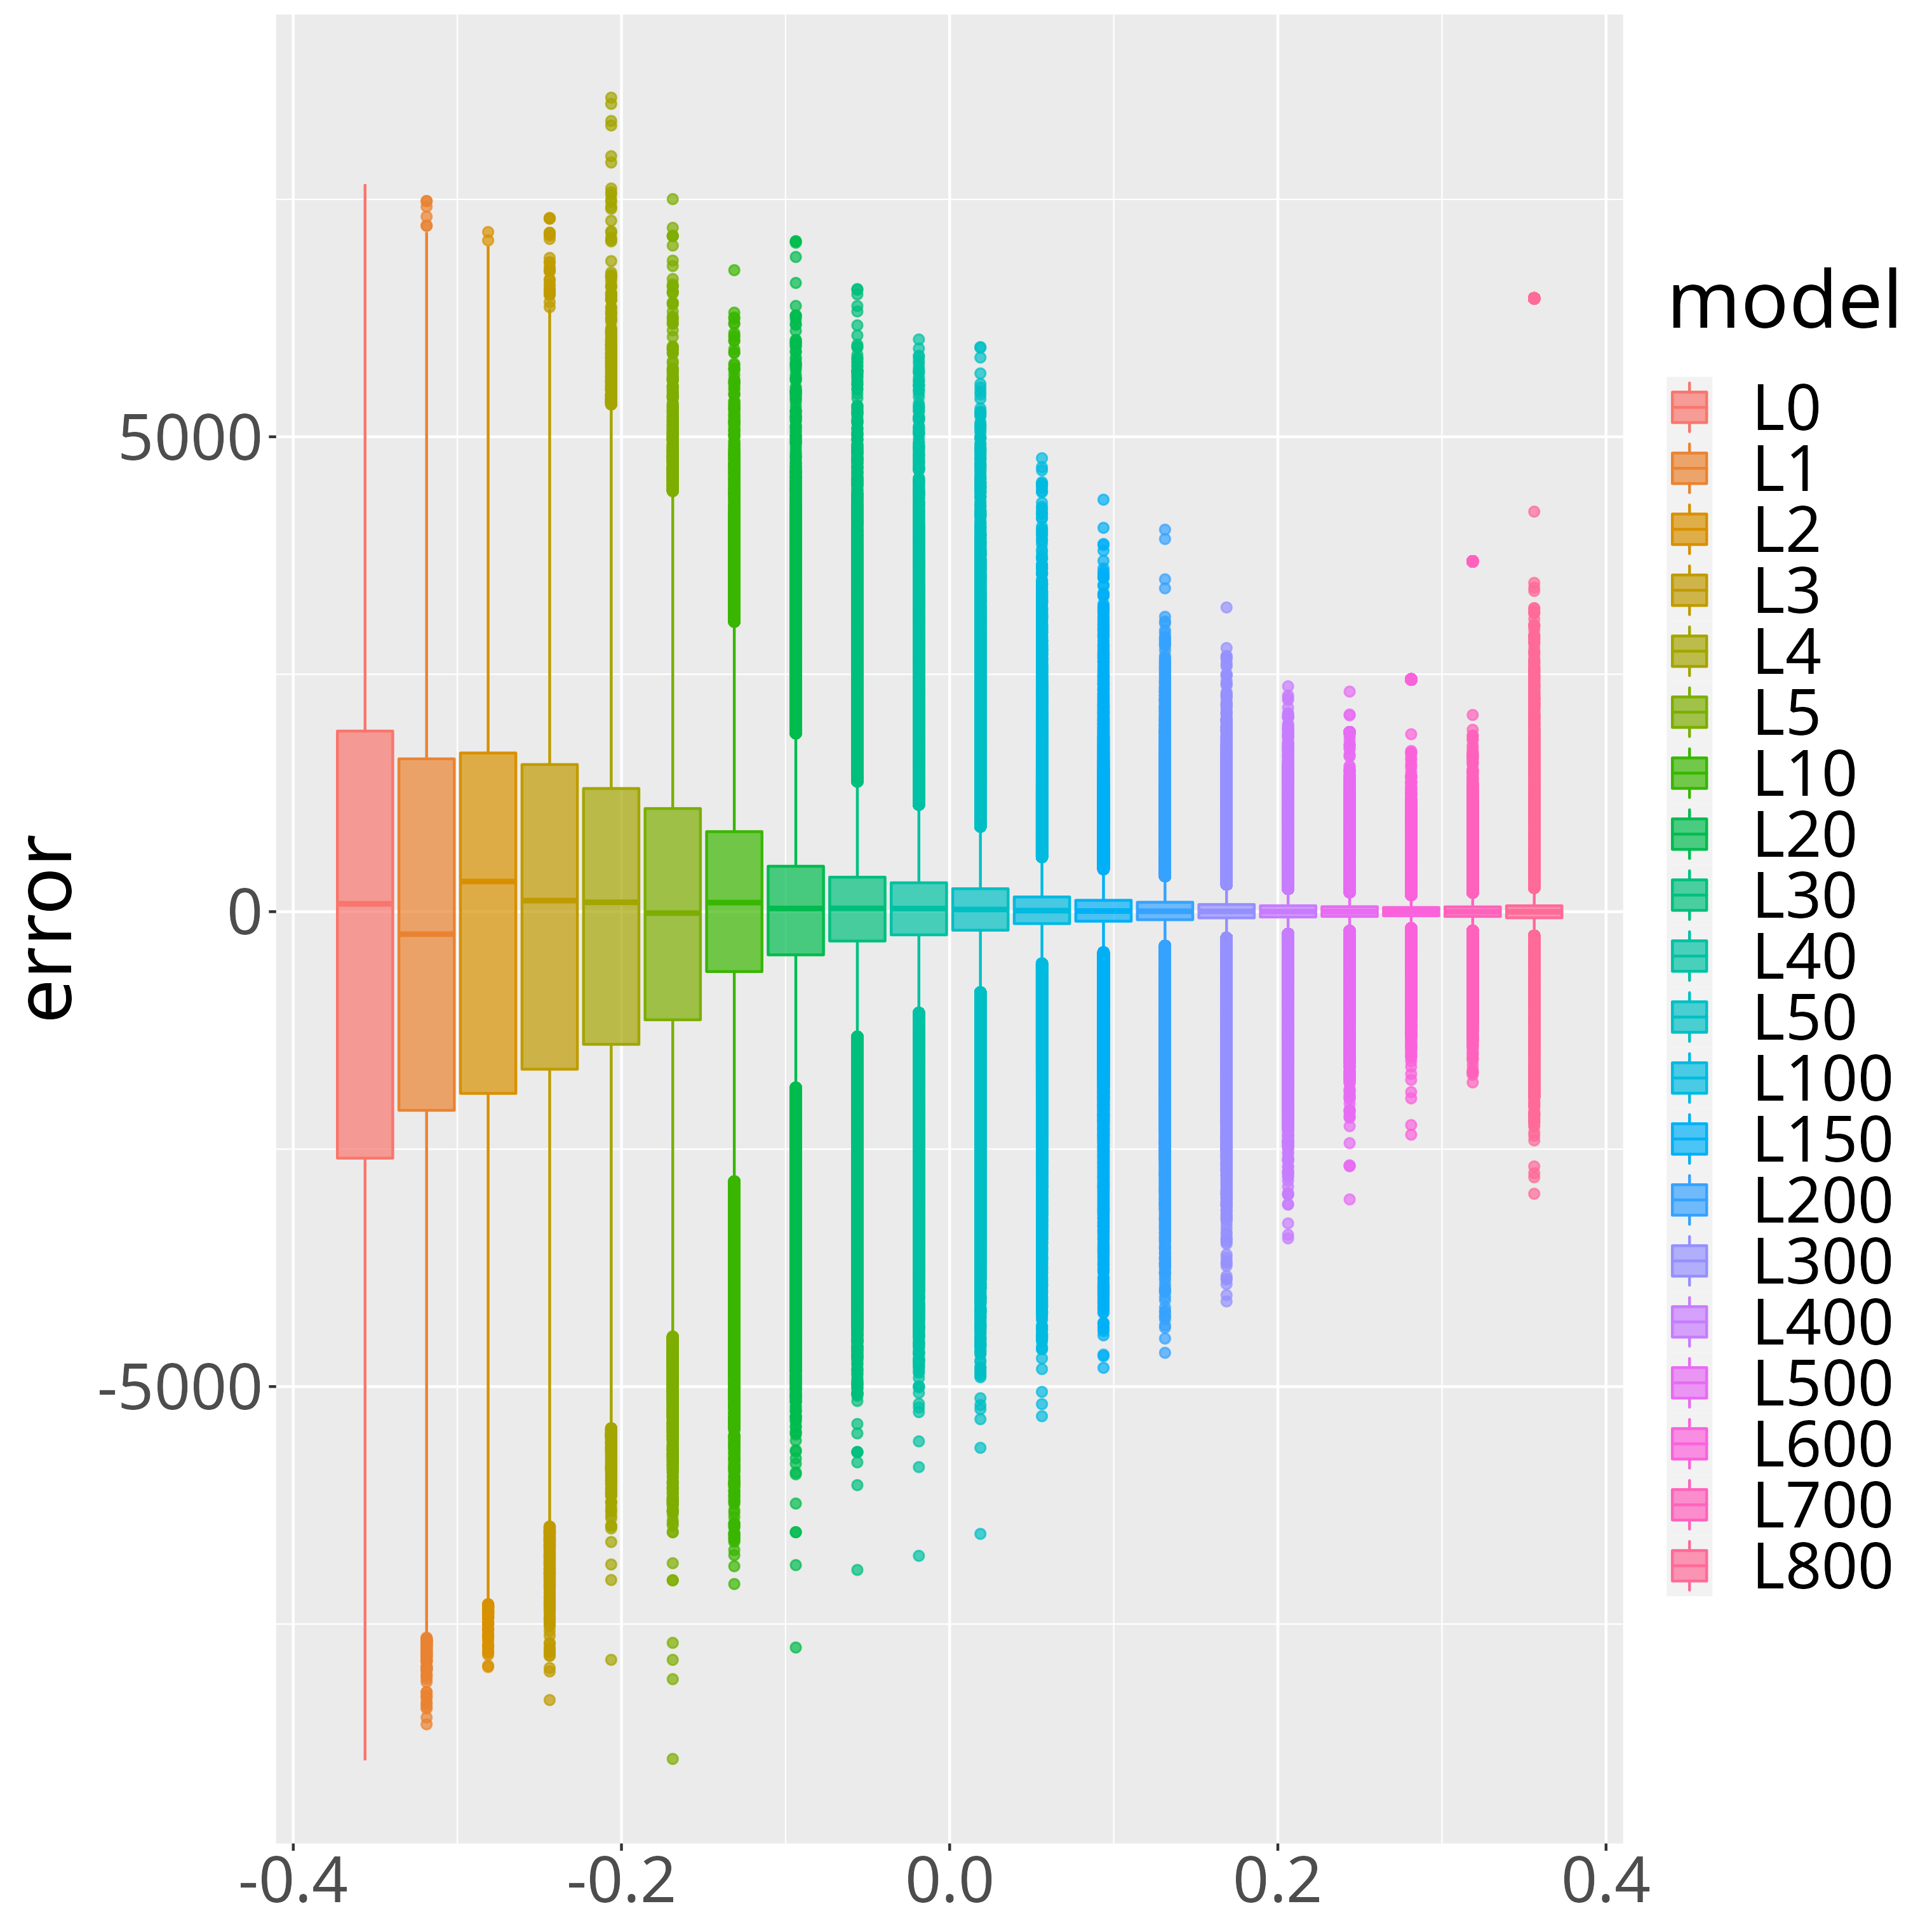
\includegraphics[width=0.9\linewidth]{media/med_error_box.png}
    \end{minipage}
    \begin{minipage}{.45\textwidth}
        \centering
            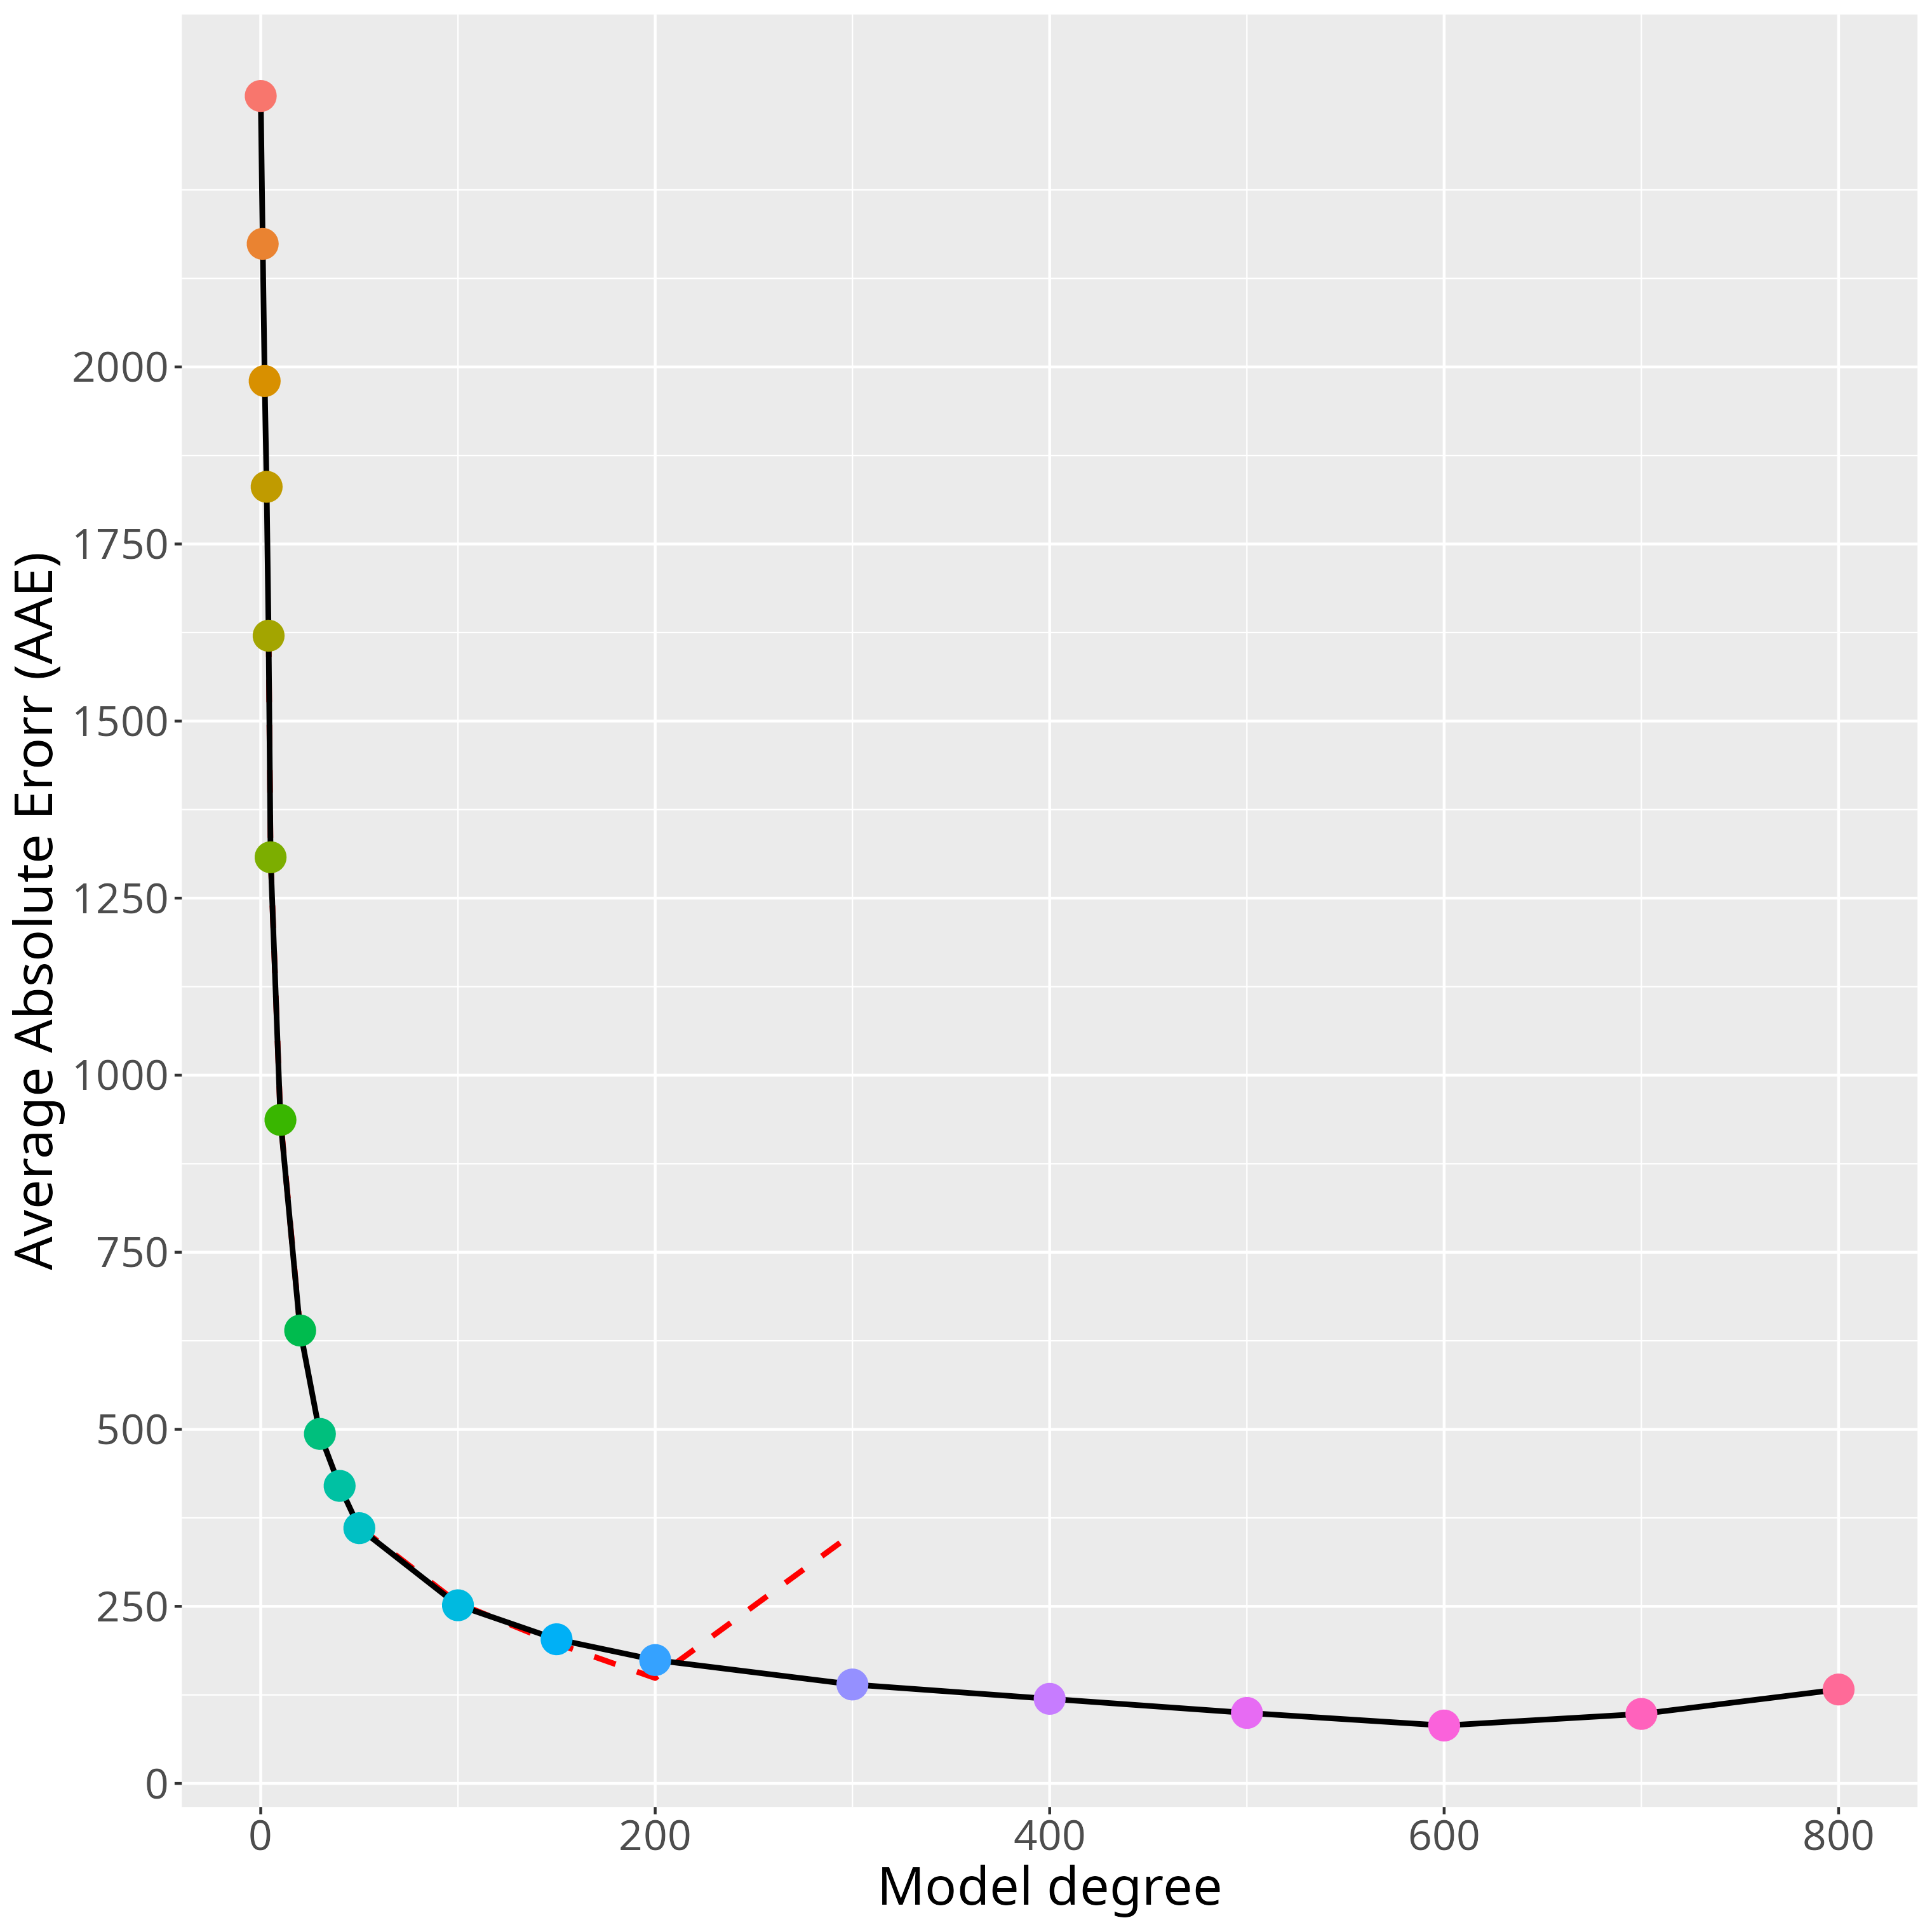
\includegraphics[width=0.9\linewidth]{media/med_err.png}
    \end{minipage}
    \caption{Boxplot of the residuals $r_i = \hat f_i - f_i$ (left) for models of degree up to $l = 800$ and the AAE associated (right)
    built on the medium dataset. The red dashed line shows the AAE($l$) of models trained on the small dataset.}
\end{figure}

Just like with the small dataset, we find that the AAE($l$) decreases as $l$ gets bigger, but there is a certain point for the which the model starts to misbehave
and the average absolute error, $\frac{1}{N}\sum_{n = 1}^N |\hat f_i - f_i|$, begins to rise. We find that the medium data set has a near optimal model at $l = 600$, with 
AAE 81.77012. We have nearly halved the AAE by increasing the degree of our model by a factor of 3. Next, we plot the distributions of the residuals for varying $l$.
\newpage

\begin{figure}
    \centering
    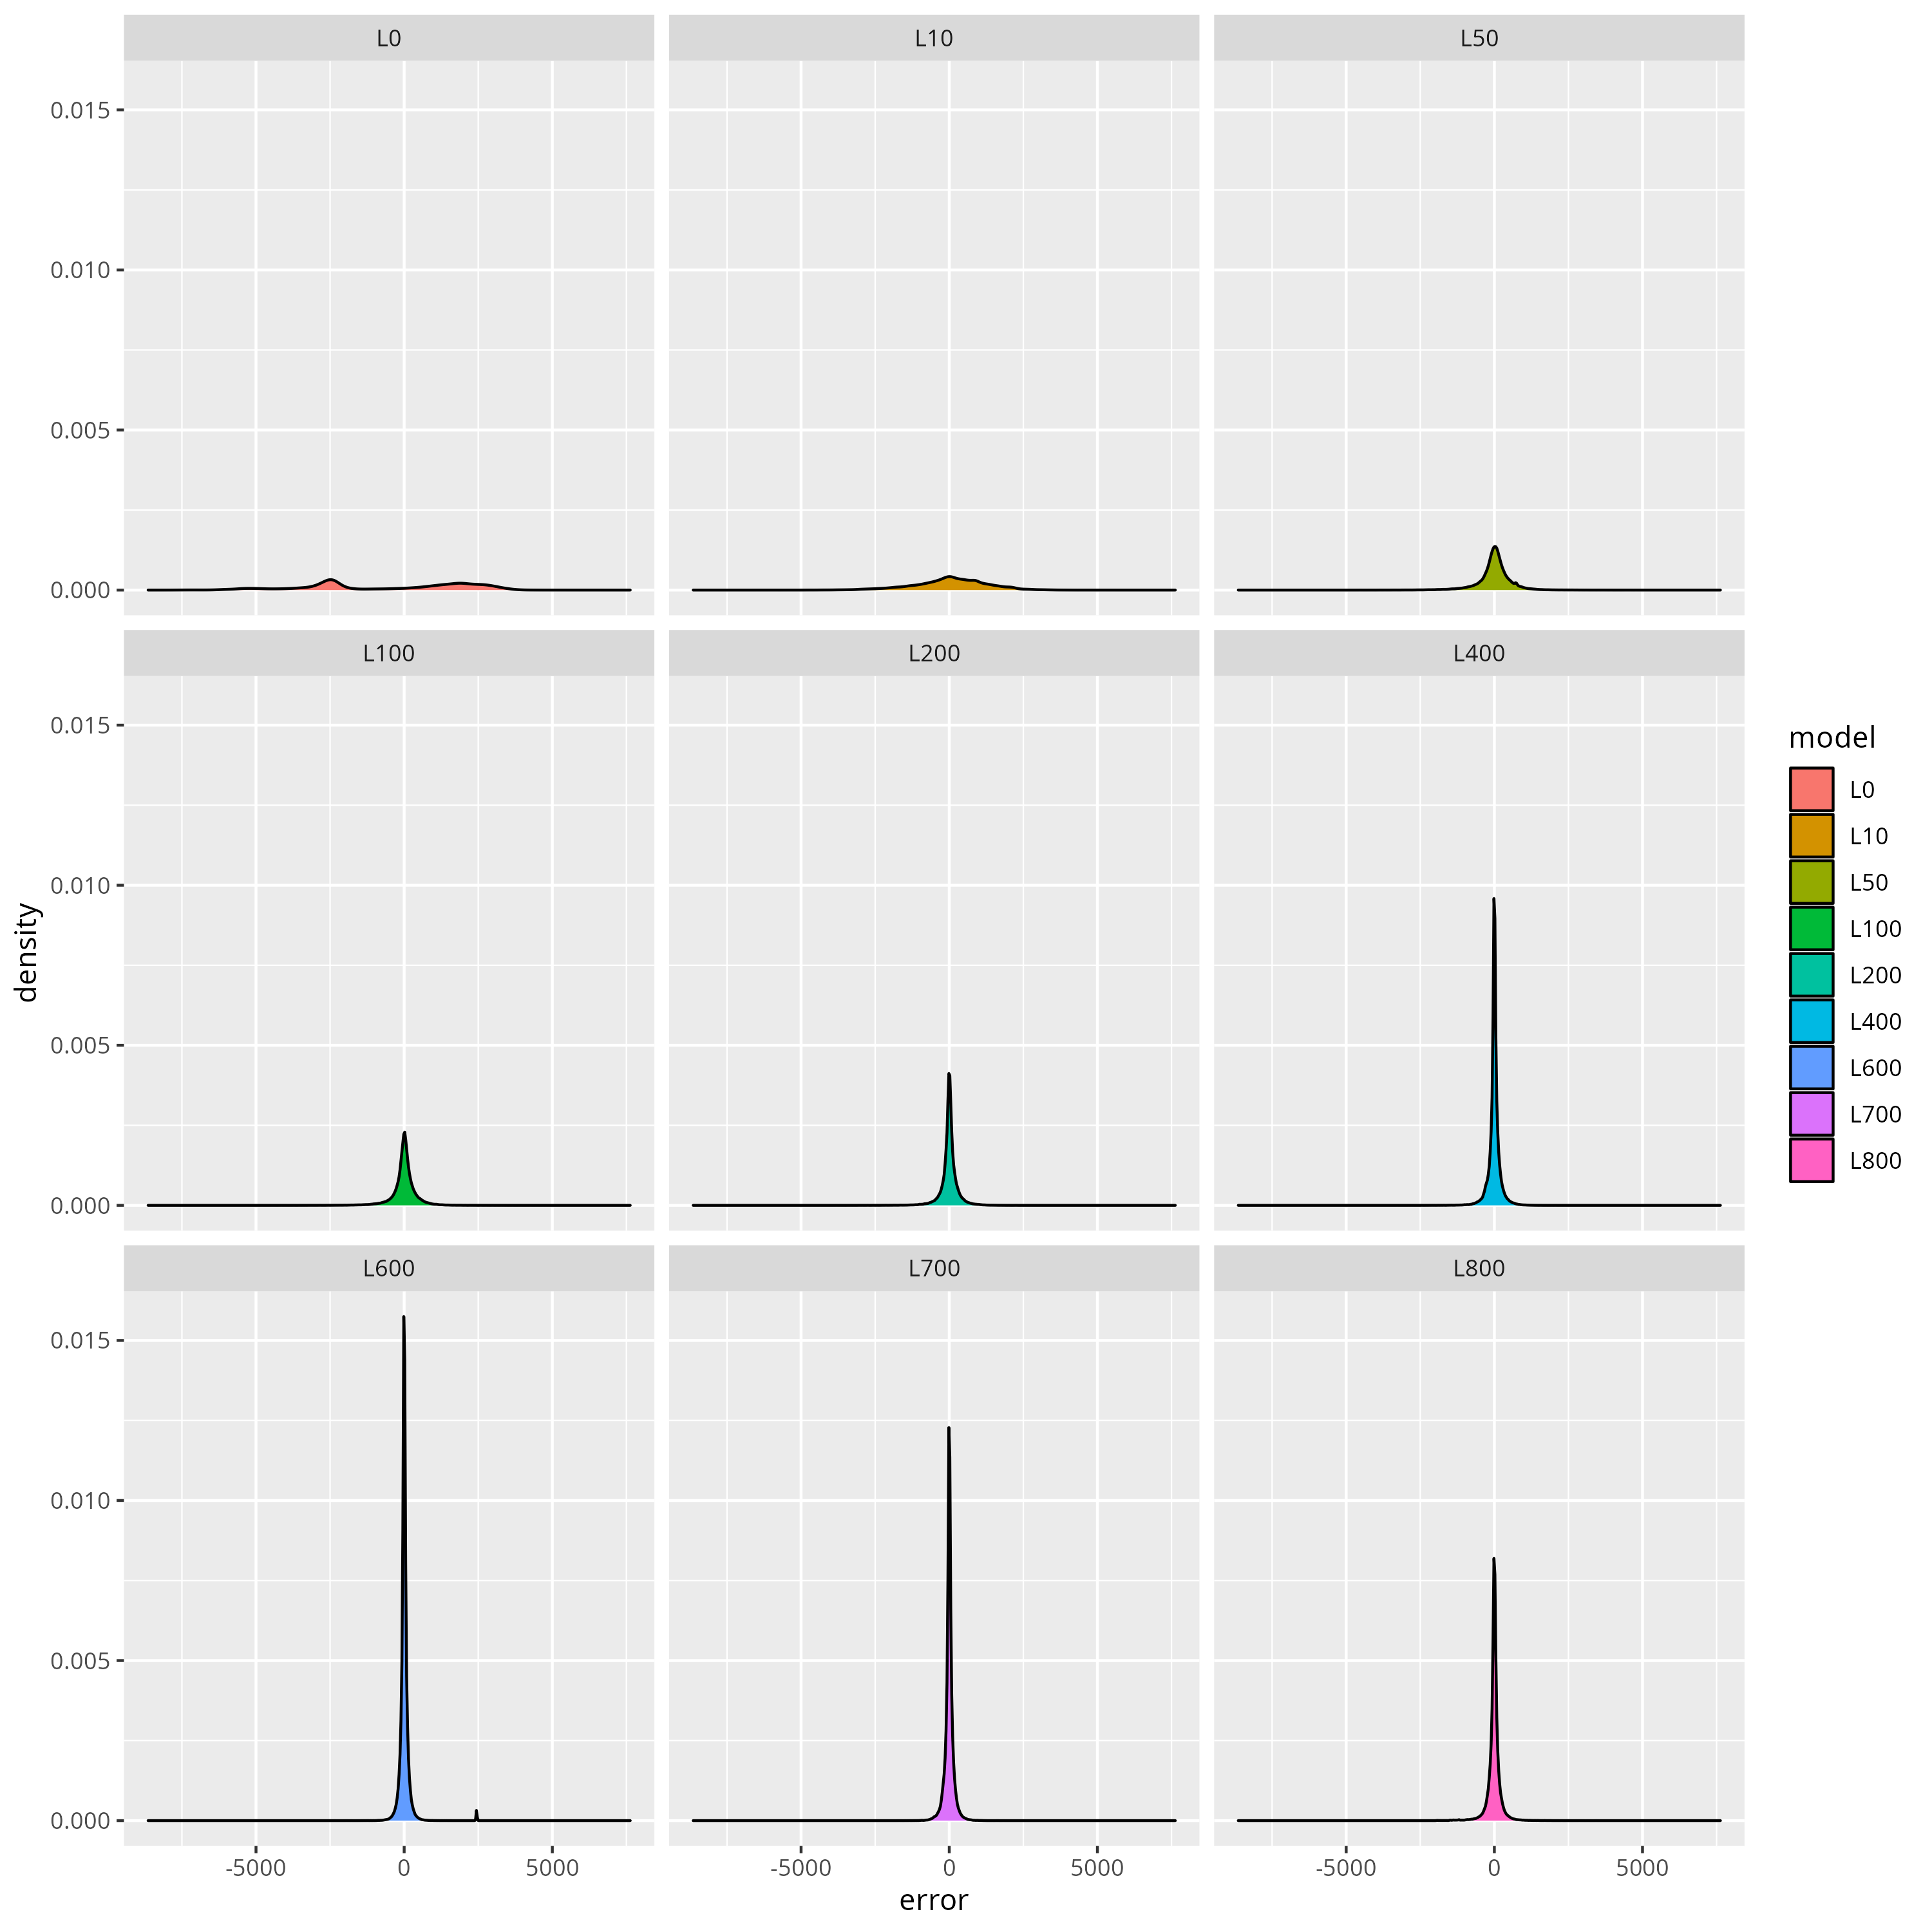
\includegraphics[width=0.85\linewidth]{media/med_err_density.png}
    \caption{Kernel density estimates for the distribution of $r_i$. The model with the lowest variance occurs at $l = 600$.}
\end{figure}

We present the result that the distribution of the residuals approximately follows a cauchy distribution. This observation is important for the analysis of our 
models because it allows us to conclude that not only do higher degree models have a lower AAE, they also have residuals which are much more tightly packed than their
lower model counterpart. For example, for a model of degree 600, we find that not only is the AES(600) = 81.77012, but also that 75$\%$ of residuals $|r_i|$ are less
than 100. If we compare this with a lower degree model, take $l = 300$ for example, we observe that 83.7\% of the residuals for a model of $l = 600$ have magnitude less 
than AES(300) = 139.704. To put this in perspective, take another look at Figure \ref{fig:earth_models}. 83.7\% of the residuals are \textit{more accurate} than the \textit{average}
prediction for the highest degree model of Figure \ref{fig:earth_models}. Conclusion: higher degree models have a lower AAE and a lower variance.

To conclude our analysis of higher degree models, we provide a table with important statistics about the residuals $r_i$.

\section{Parallelization} 

In this section we present our parallelization algorithms and evaluate their scalability and efficiency. 

\subsection{Implementation}

The meat of our program and most computationally expensive component is the computation of the all of the coefficients up until a certain $l_{\mathrm{max}}$. 

\subsubsection{OpenMP}

The first loop that I tried to parallelize with OpenMP was the internal for loop computing the summation of N observations of $f(\phi_i, \theta_i)$ that needs to be run for each $C_l^m, S_l^m$ pair. 
This seems completely logical, since the summation is the largest loop and we ideally want to reduce the overhead associated with parallel mechanisms like spawning new threads. 
However, we quickly observed that models of a sufficiently large degree were actually running slower with this parallel paradigm. We posit that even though we targeted the largest loop,
we failed to consider that for every value $(l, m)$ we are incurring overhead by splitting. For a model of $l = 100$ we end up with over 10,000 parallelization entry points.

    Our second attempt at parallelization targeted the \textit{outer} loop that iterates all the valid $(l, m)$ pairs, computing $C_l^m, S_l^m$. This implementation, which only split 
    apart a single for-loop, was immediately successful.
\subsubsection{OpenMPI}

After wrangling some indexing errors introduced when adapting to OpenMPI's memory model, we managed to succesfully compile a parallel mpi implementation
of our algorithm.

\subsection{Benchmark}

The initial tests of scalability were performed on a desktop with a 12 core cpu. We repeated the computation of models with degre 50, 100, and 200 ten times, then 
plotted the average runtime of these trials and other pertinent statistics.


\begin{figure}[h!]
\begin{minipage}{0.45\linewidth}
    \centering
    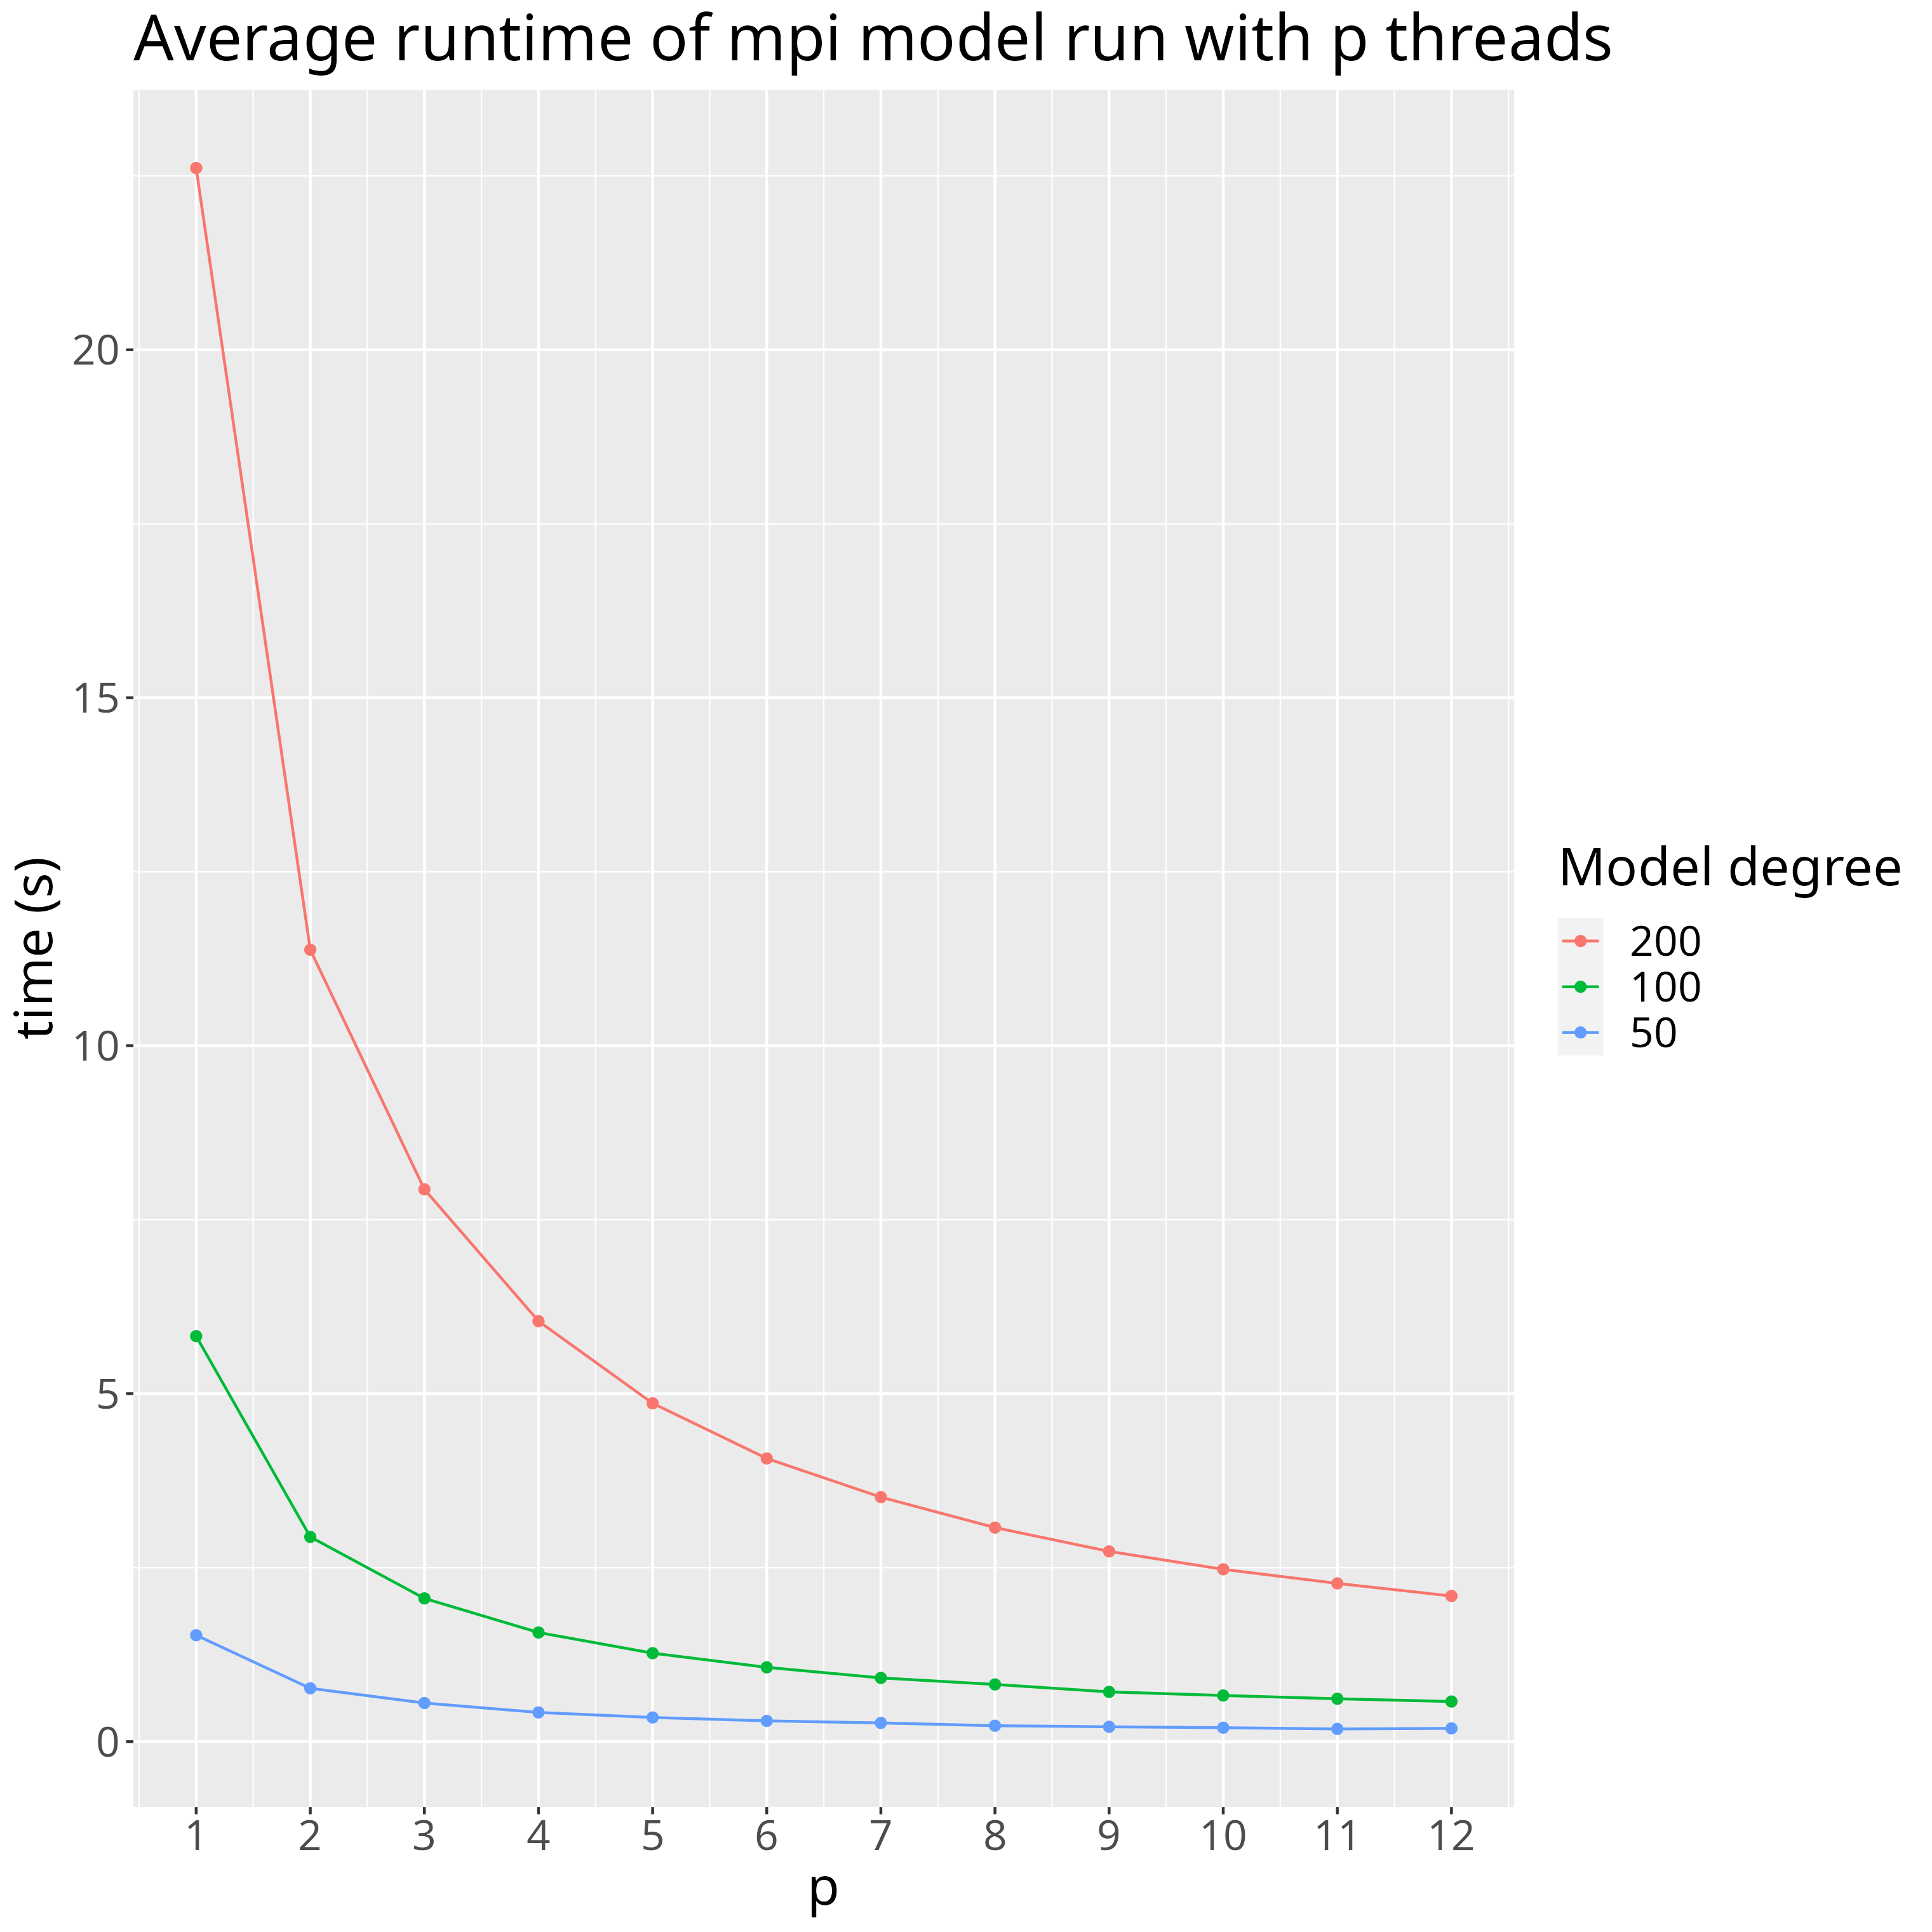
\includegraphics[width=0.95\textwidth]{media/mpi_runtime.png}
\end{minipage}
\begin{minipage}{0.45\linewidth}
    \centering
    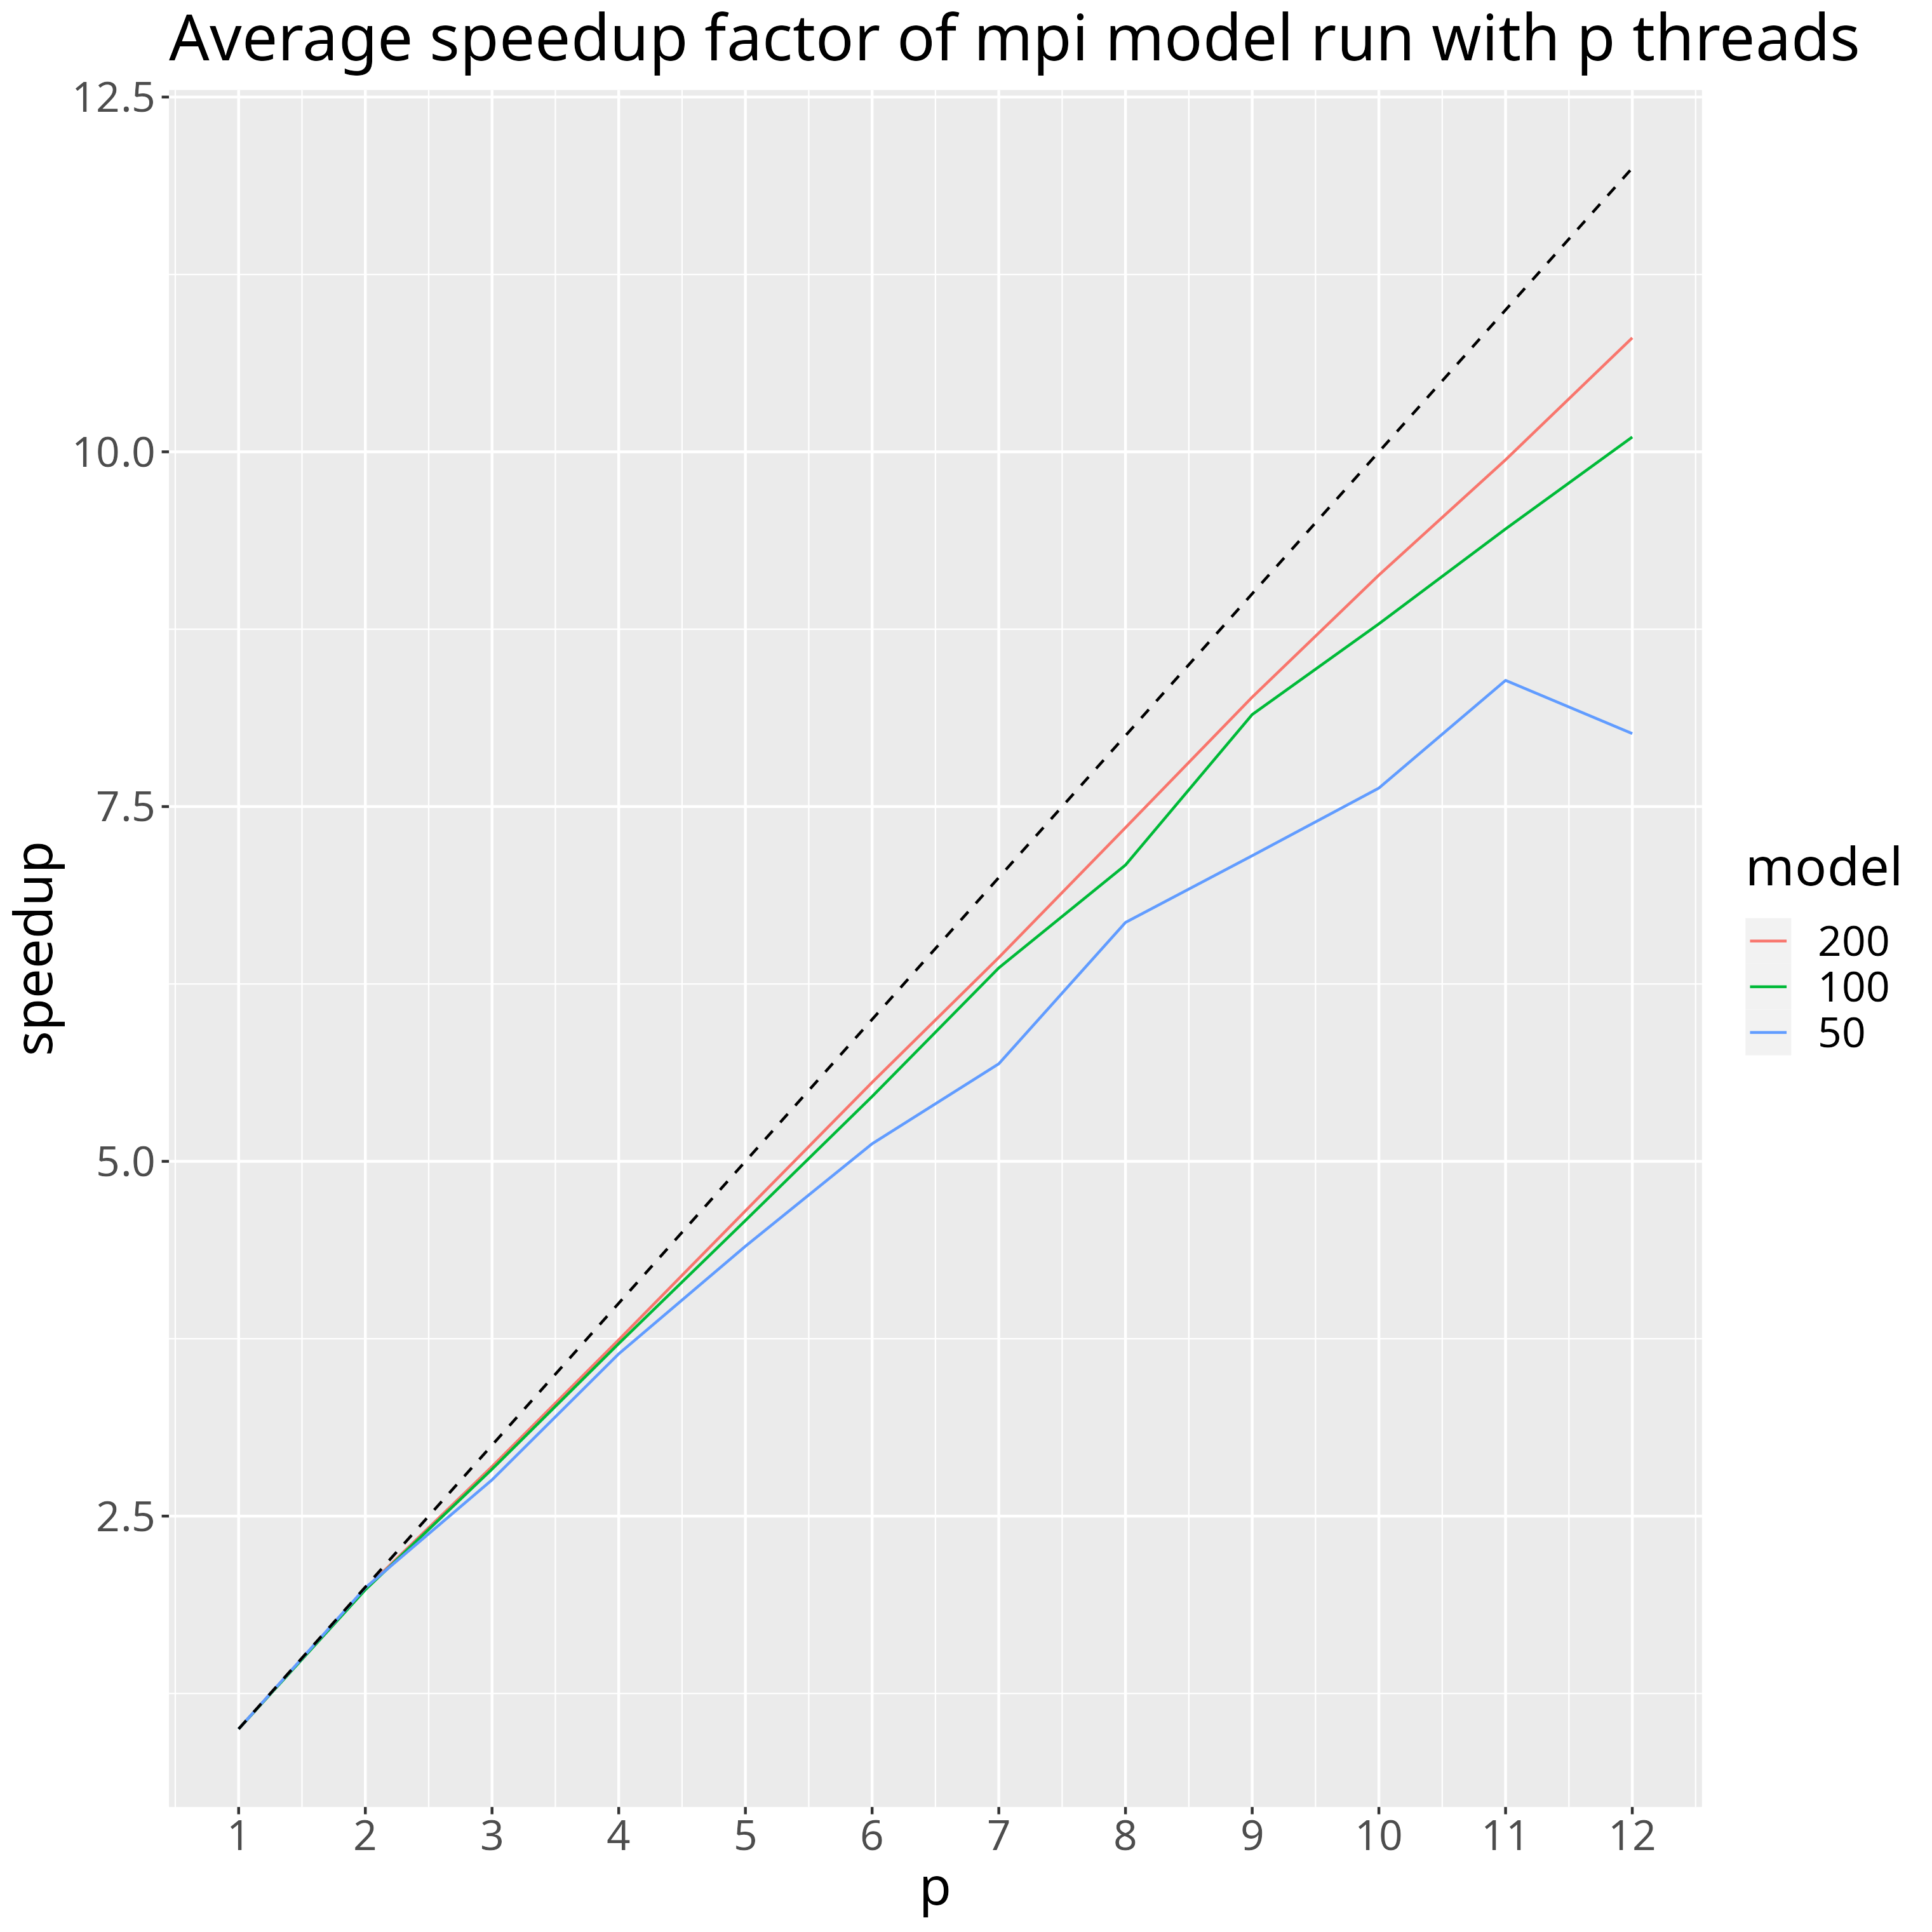
\includegraphics[width=0.95\textwidth]{media/mpi_speedup.png}
\end{minipage}
\caption{For models degree $l \in [50, 100, 200]$ we computed the average runtime across 10 executions. On the left-hand side we show how the runtime is affected
by introducing more threads. On the right-hand side we plot the speedup coefficient, $S(p) = \frac{T_s}{T_p}$, defined as the runtime in sequential divided by the 
runtime with p mpi processes. The dashed line shows the ideal speedup factor, $S(p) = p$.}
\end{figure}

For a sufficiently large model (in the case of the small data set, $l = 200$), the speedup factor for mpi programs ran with up to 12 processes approaches ideal values. We cannot
overstate the significance of this result. \textbf{The speedup factor of computing our models of degree $l$ with $p$ mpi processes approaches ideal levels.}

\begin{figure}
    \centering
    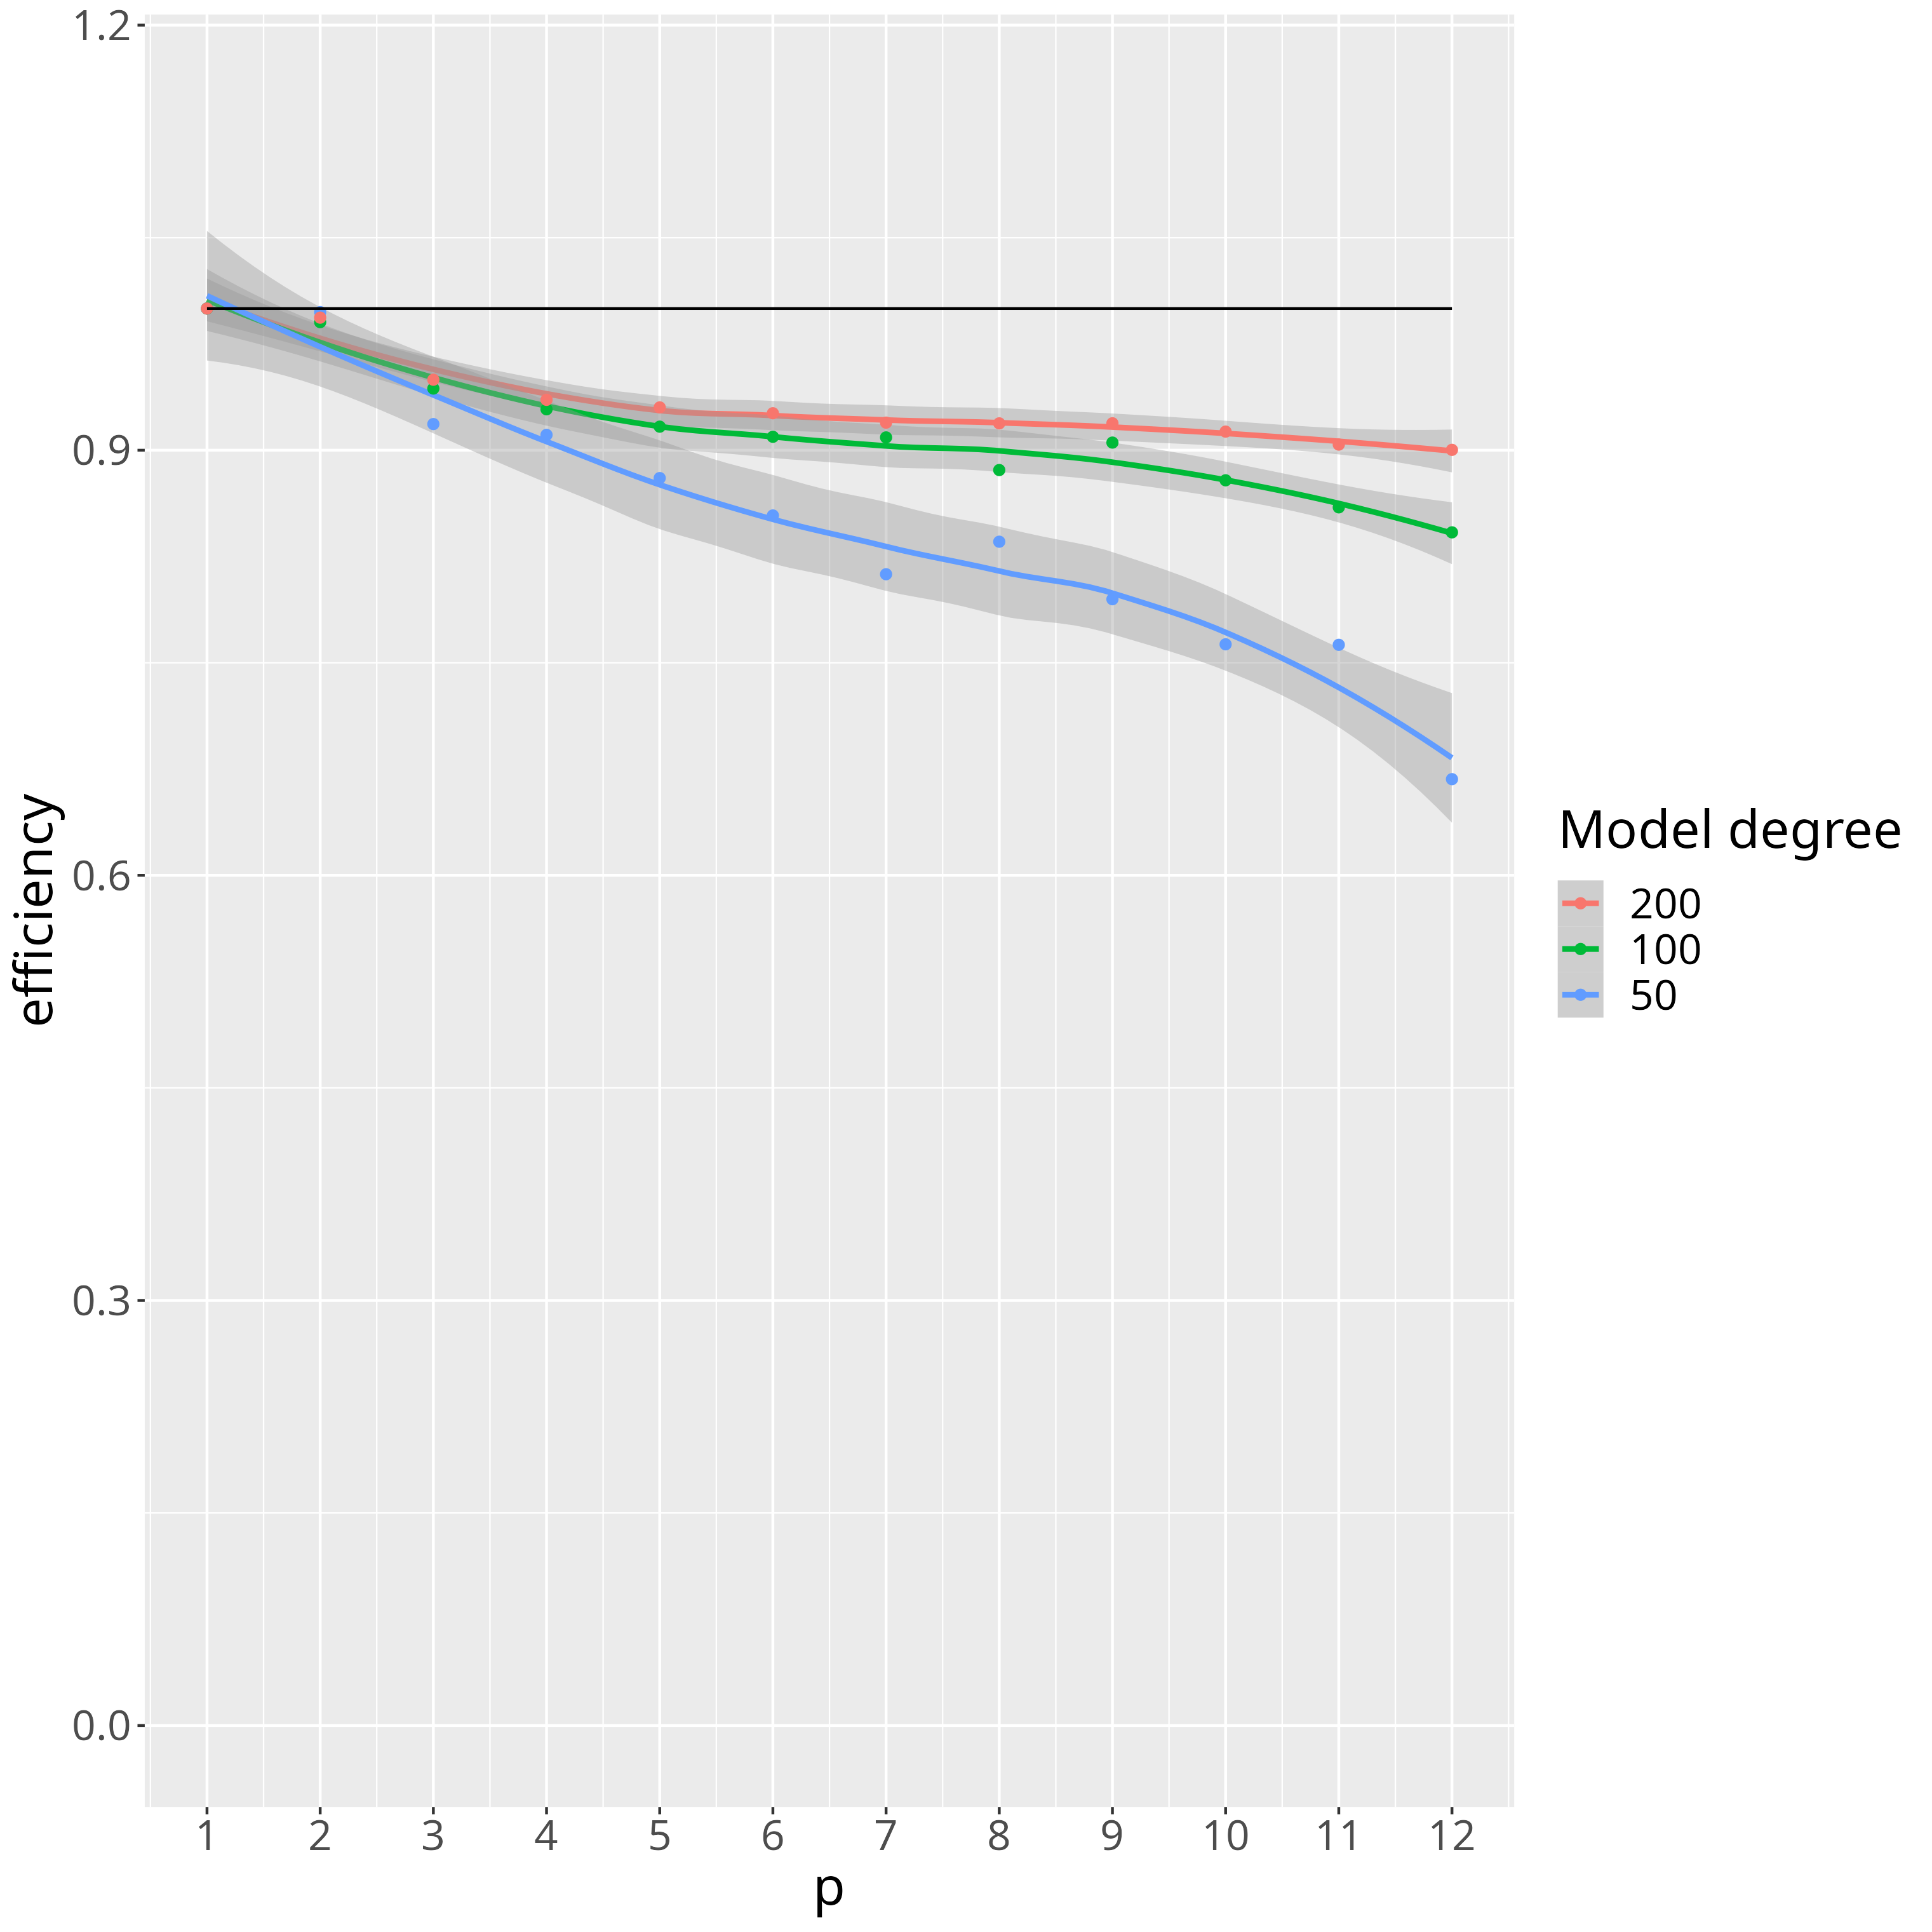
\includegraphics[width=0.5\linewidth]{media/mpi_efficieny.png}
    \caption{The efficiency, $\frac{S(p)}{p}$, is a test of how much of $p$ threads' theoretical computation power is
    being harnessed. An ideal system has an efficiency of 1.}

\end{figure}

\section{Final phase}

In this section we present the implementation of a final optimization which makes use of the fact that we can compute a given $(C_l^m, S_l^m)$
independly from all the other coefficients.

To provide context, we begin by establishing some new notation.

\subsection{Ranges}

Let $C_l^*$ and $S_l^*$ denote the set of Laplace Series coefficients whose degree is equal to $l$.
\begin{align*}
   C_l^* &= \{C_l^0, C_l^1, ..., C_l^l\} \\
   S_l^* &= \{S_l^0, S_l^1, ..., S_l^l\} 
\end{align*}

For example, $C_4^* =\{C_4^0, C_4^1, C_4^2, C_4^3, C_4^4\}$. Additionally, Let 
$C_{[a, b]}$ and $S_{[a, b]}$ denote the union of the coefficients of degree $a$ through $b$:

\begin{align*}
    C_{[a, b]} &= \bigcup_{l = a}^{b} C_l^* \\
    S_{[a, b]} &= \bigcup_{l = b}^{b} S_l^*
\end{align*}

In this section we refer to them as \textbf{ranges}. To elucidate this notation, we have

\begin{align*}
    S_{[2, 3]} &= S_2^* \cup S_3^* \\
               &= \{S_2^0, S_2^1, S_2^2\} \cup \{S_3^0, S_3^1, S_3^2, S_3^3\} \\
    C_{[0, 4]} &= C_0^* \cup C_1^* \cup C_2^* \cup C_3^* \cup C_4^* \\
               &= \{C_0^0\} \cup \{C_1^0, C_1^1\} \cup \{C_2^0, C_2^1, C_2^2\} \cup \{C_3^0, C_3^1, C_3^2, C_3^3\} \cup \{C_4^0, C_4^1, C_4^2, C_4^3, C_4^4\} \\
               &= \{C_0^0, C_1^0, C_1^1, C_2^0, C_2^1, C_2^2, C_3^0, C_3^1, C_3^2, C_3^3, C_4^0, C_4^1, C_4^2, C_4^3, C_4^4\} 
\end{align*}

Any range can easily be partioned into a union of disjoint subranges, a fact that will be exploited to save an enormous amount of computational time when constructing
increasingly larger models. For example, $C_{[0, 7]}$ can be partitioned into $C_{[0, 3]} \cup C_{[4, 7]}$. $|C_l^*|$, the cardinality of $C_l^*$, is equal to 
$\frac{(l + 1)(l + 2)}{2}$. We don't immediately see what $|C_{[a, b]}|$ might be equal to but we'd like to find an expression for the cardinality of a general range.
We solve for this expression by rewriting $C_{[0, b]}$ as a union of disjoint subranges:

\begin{align}
    C_{[0, b]} &= C_{[0, a - 1]} \cup C_{[a, b]} \\
    |C_{[0, b]}| &= |C_{[0, a - 1]}| + |C_{[a, b]}| \\
    \frac{(b + 1)(b + 2)}{2} &= \frac{a(a + 1)}{2} + |C_{[a, b]}|
\end{align}

Solving for $|C_{[a, b]}|$ yields 
\begin{equation}
    |C_{[a, b]}| = \frac{(b + 1)(b + 2) - a(a + 1)}{2} \label{fig:cardinality}
\end{equation}

Thus $\mathcal{M}_{l_\mathrm{max}}$, a model of degree $l_{\mathrm{max}}$, can be written as $\mathcal{M}_{l_\mathrm{max}} = C_{[0, l_{\mathrm{max}}]} \cup S_{[0, l_{\mathrm{max}}]}$. Assuming that we've already computed the coefficients for a model 
$\mathcal{M}_l$, all we need to compute a model $\mathcal{M}_{l + n}$ is to compute the new coefficients $C_{[l + 1, l + n]}$ and $S_{[l + 1, l + n]}$!

Let's explore the consequences of this observation using a concrete example. Suppose we have a precomputed model $\mathcal{M}_{500}$ for the high data set. If we would 
like to compute a model $\mathcal{M}_{600}$ using traditional means, we would need to compute $\frac{(601)(602)}{2} * 2 = 361802$ new coefficients. If, however, we leverage the fact
that each $C_l^m$ and $S_l^m$ can be computed independently, we are only required to compute the coefficients $C_{[501, 600]}$ and $S_{[501, 600]}$. Computing
$|C_{[501, 600]}|$ gives us $\frac{(601)(602) - (501)(502)}{2} * 2 = 110300$ new coefficients to compute, which is more than 3 times fewer than for a classic model. What's significant is that 
once model of a certain degree has been computed, we don't forget the coefficients for subsequent runs. Practically speaking, this optimization paves the way for computation of models with degree 
in the thousands. A single run with 128 mpi threads to compute $\mathcal{M}_{400}$ clocked in at 180.546s, $\mathcal{M}_{500}$ in 289.548s, and $\mathcal{M}_{600}$ in 442.99s for the \texttt{ETOPO1\_hi.csv} dataset 

We have already shown that the coefficients $C_l^m$ and $S_l^m$ computed via quadrature are independent of the $l_\mathrm{max}$ of a model. Therefore by storing the coefficients values of computed models in a 
binary file we accumulate a corpus of models of increasing degree. Storing the previously computed coefficients allows us to spread out the computation of a 
very large model across separate executions. The original quadrature model (and also the least-squares approach) computes all of the coefficients $(l + 1)(l + 2)$ 
in a single program execution. Once the necessary machinery is in place, everytime we run our program we will be inexorably advancing towards a higher degree 
model, instead of wasting time reevaluating coefficients that may have already been computed hundreds of times throughout testing.

    Imagine the difference in wealth accumulated of a fictitious character whose bank account gets reset to zero every single data, compared to someone who only ever makes
deposits and that persist across days.

\section{Conclusion}

Instead of calculating the model with a direct method that runs in $O(Nl_{max}^4)$ time, We propose a hybrid model that first directly computes the coefficients in $O(Nl_{max}^2)$ time then 
iteratively improves the MSE via stochastic methods running in $O(n_{training}n_{sample}l_{max}^2)$ time.

Results are to follow :)





\appendix
\section{Spherical Coordinates Transformation}

The data sets \verb|ETOPO1_*.csv| provided by NASA represent spherical coordinates in an unconventional format: $$(\phi, \lambda) \in [-\frac{\pi}{2}, \frac{\pi}{2}] \times [-\pi, \pi] $$ where $\phi$ refers to the latitude
and $\lambda$ refers to the longitude. In this section we outline the transformation from NASA's coordinate system to the ISO standard representation and prove equivalence between (1) and the Project presentation's $f(\phi, \lambda)$.

To avoid confusion, we denote the spherical coordinate pair in ISO coordinates as $(\theta_{iso}, \phi_{iso})$ and NASA's coordinate scheme as $(\phi_{nasa}, \lambda_{nasa})$.
We remark that the polar angle $\theta_{iso}$ is simply equal to $\frac{\pi}{2} - \phi_{nasa}$. We corroborate this fact by remarking that a latitude of $\phi_{nasa} = 0$ corresponds to a polar
angle of $\phi_{iso} = \frac{\pi}{2}$. Conveniently, the longitude $\lambda_{nasa}$ is equivalent to the azimuthal angle $\phi_{iso}$.

\begin{proposition} Let the spherial coordinate pairs $(\theta_{iso}, \phi_{iso})$, $(\phi_{nasa}, \lambda_{nasa})$ be defined as above. 
    \begin{equation*}
        f(\theta_{iso}, \phi_{iso}) \equiv f(\phi_{nasa}, \lambda_{nasa})
    \end{equation*}

    
\end{proposition}



\begin{proof}
    $f(\phi_{nasa}, \lambda_{nasa})$ is defined in the Project proposal as 
    \begin{align} \label{eq:project_def} 
        f(\phi_{nasa}, \lambda_{nasa}) &= \sum_{l = 0}^{+\infty}\sum_{m = 0}^l \bar P_l^m(\sin\phi_{nasa})[C_l^m\cos m\lambda_{nasa} + S_l^m \sin m \lambda_{nasa}] \\ 
                                       &= \sum_{l = 0}^{+\infty}\sum_{m = 0}^l \bar P_l^m(\sin(\pi/2 - \theta_{iso}))[C_l^m\cos m\phi_{iso} + S_l^m \sin m \phi_{iso}] \\
                                       &= \sum_{l = 0}^{+\infty}\sum_{m = 0}^l \bar P_l^m(\cos\theta_{iso}))[C_l^m\cos m\phi_{iso} + S_l^m \sin m \phi_{iso}] \\
                                       &\equiv f(\theta_{iso}, \phi_{iso})
    \end{align}

\end{proof}

\nocite{*}

\bibliography{ppar}
\bibliographystyle{ieeetr}

\end{document}

